\documentclass[a4paper, 12pt]{article}
\usepackage[utf8]{inputenc}
\usepackage[UKenglish]{isodate}
\usepackage[UKenglish]{babel}
\usepackage[numbered, framed]{matlab-prettifier}
\usepackage{graphicx}
\usepackage{caption}
\usepackage{subcaption}
\usepackage{wrapfig}
\usepackage{amsmath}
\usepackage[nottoc]{tocbibind}
\usepackage{wrapfig}
\usepackage[section]{placeins}
\usepackage{multicol}

\lstset{
  style = Matlab-editor,
  basicstyle = \footnotesize,
  mlshowsectionrules = true,
  tabsize=2,
}

\title{
	{EE2-08C - Numerical Analysis of ODEs using Matlab - Coursework 2017 \\ Group 30}
}
\author{Yijie Chen, CID: 01051752 \\ Mostafa Hagras, CID: 01053843\\ David Rovick, CID:  01070823\\ Tanay Verma, CID: 00929784 \\ Pu Yang, CID: 01082988}
\begin{document}
\maketitle
\tableofcontents

\newpage

\section{RL Circuit}

\begin{figure}[h]
\centering
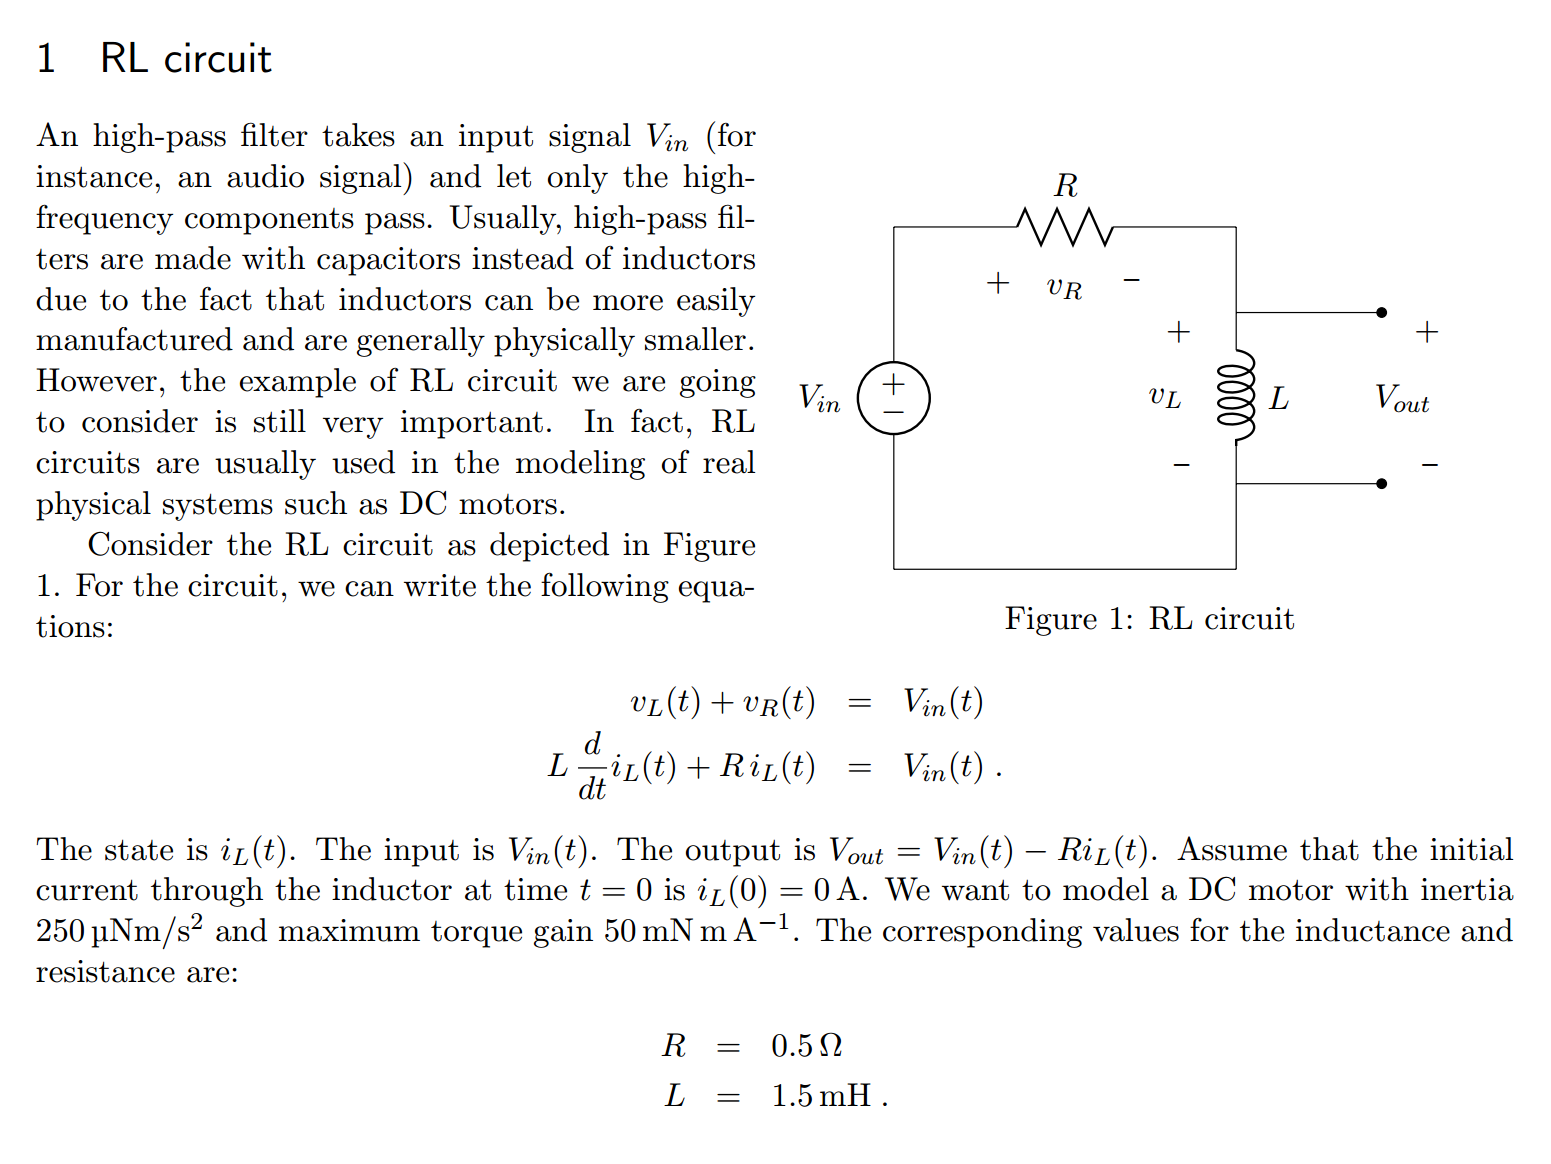
\includegraphics[width=\textwidth]{ex1/q.PNG}
\caption{Given question}
\end{figure}

In this exercise, we need to use Heun, Midpoint and Ralston method to calculate the output of the RL series circuit.

\subsection{Step Signal}

The step signal with amplitude $5.5V$:\par

Since inductor is in series with resistor, we got:\par
\[V_{in} = iR + L\frac{di}{dt}\]
By rearranging the equation we can get:\par
\[\frac{dt}{L} = \frac{di}{V - iR}\]
Integrating both sides, we get:\par
\[\int_{0}^{t} \frac{dt}{L} = \int_{0}^{i}\frac{di}{V - iR}\]
Use substitution let z = V - iR: 
\[\frac{t}{L} = -\frac{1}{R}\int \frac{dz}{z}\]
Then we get:\par
\[-\frac{Rt}{L} = ln(V - iR)\]
\indent limit from 0 to i.
After substituting limit in the equation above, we now have:\par
\[-\frac{Rt}{L} = ln(\frac{V - iR}{V}) \Rightarrow e^{-RT/L} = e^{ln(\frac{V - iR}{V})}\]
\[e^{-RT/L} = e^{ln(\frac{V - iR}{V})} \Rightarrow e^{-RT/L} = \frac{V - iR}{V}\]
Finally, we get the equation (1).
\begin{equation}\label{Exp Iout}
I_{out}=\frac{V_{in}}{R}(1-e^{-RT/L})
\end{equation}
\begin{equation}\label{Exp Vout}
V_{out}=V_{in}(e^{-RT/L})
\cite{rlcircuitprove}
\end{equation}

\begin{figure}
      \centering
      \begin{subfigure}[b]{0.4\textwidth}
            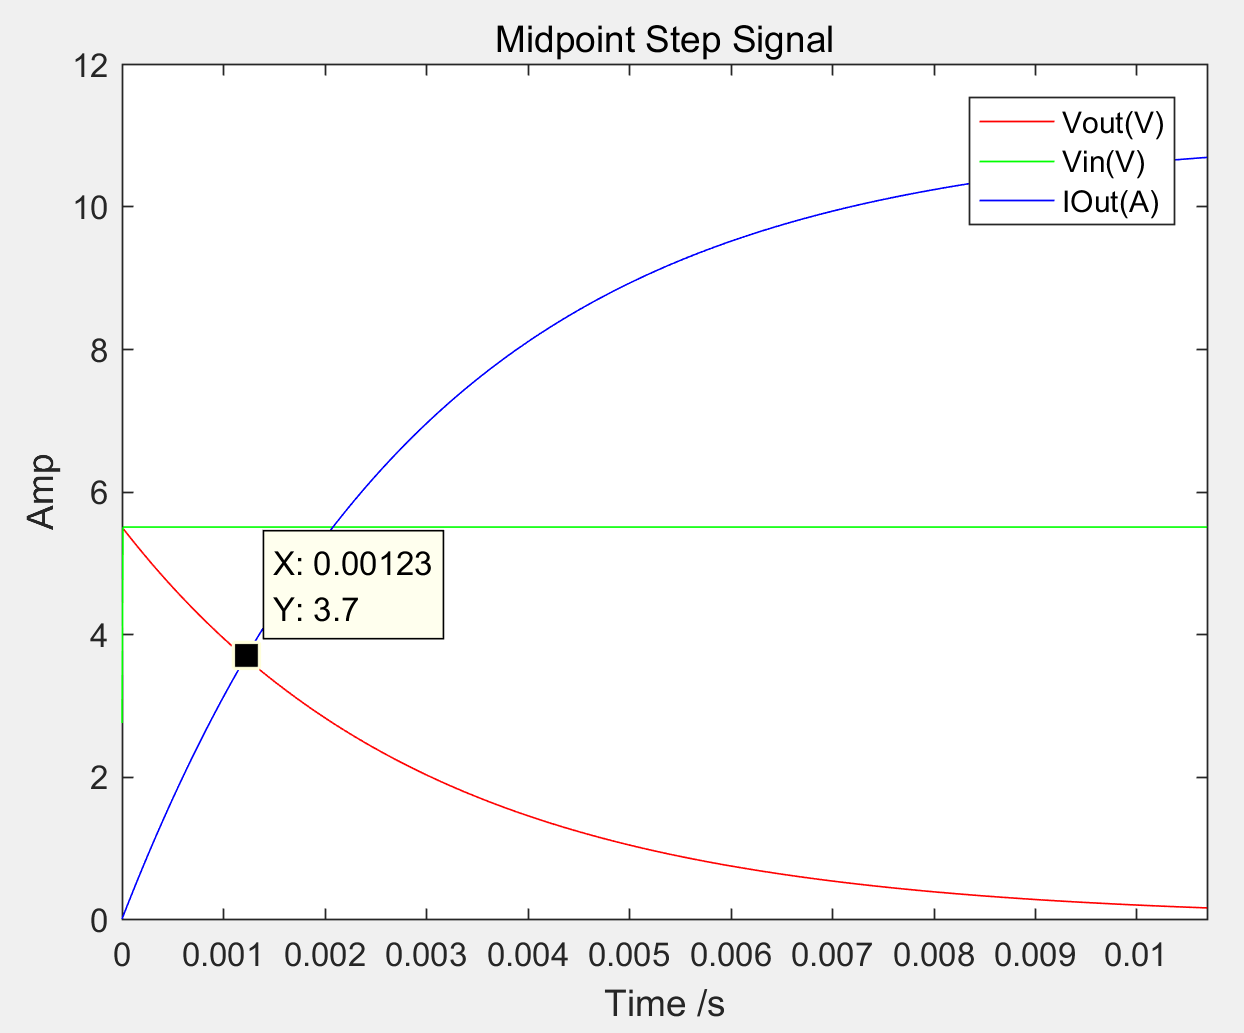
\includegraphics[width=\textwidth]{ex1/midpoint_step.PNG}
            \caption{Midpoint method}
      \end{subfigure}
      ~
      \begin{subfigure}[b]{0.4\textwidth}
            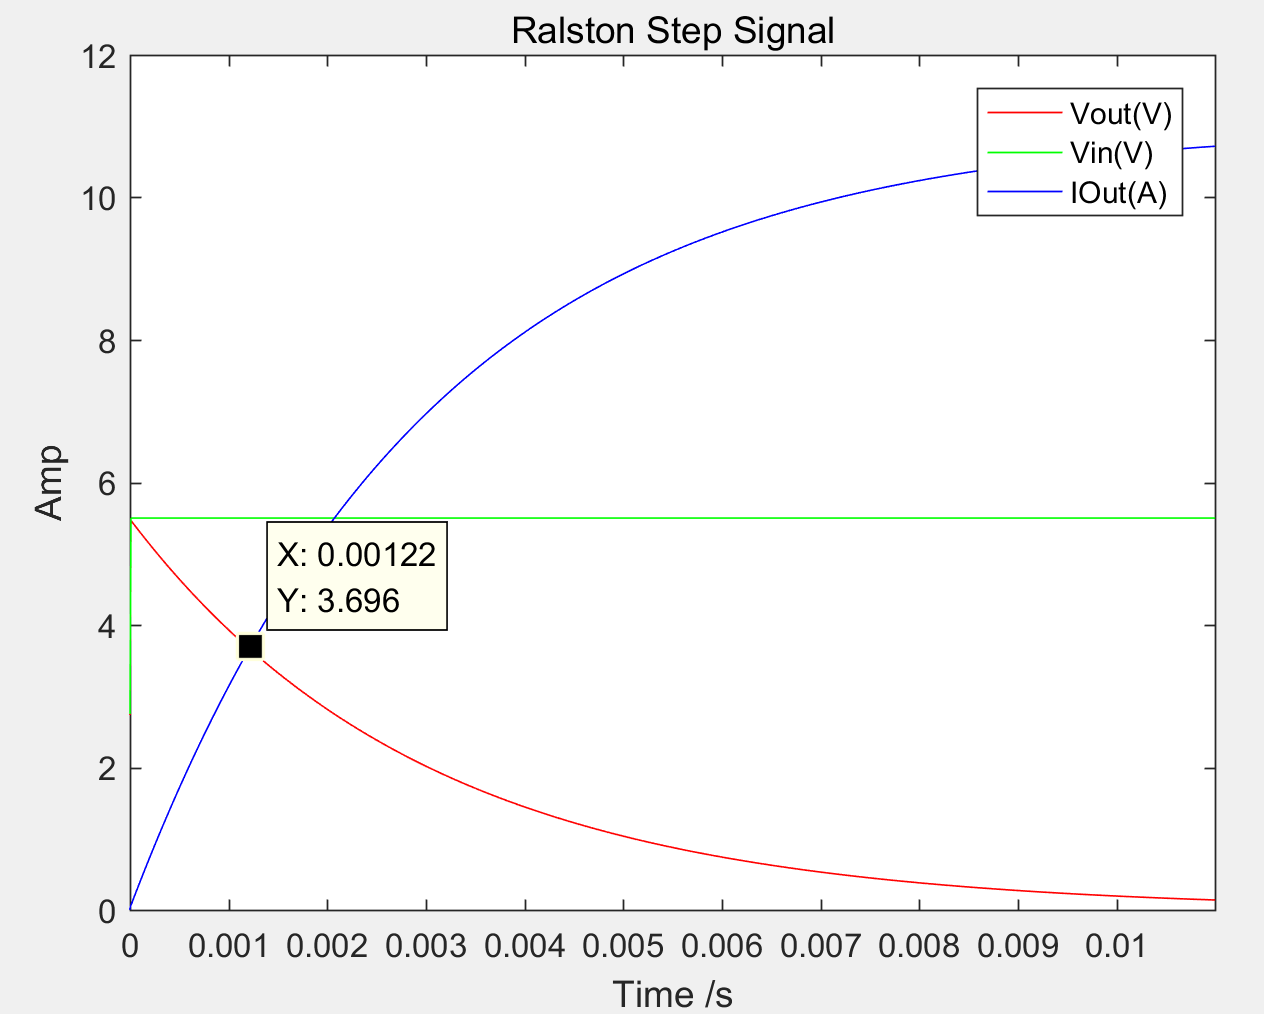
\includegraphics[width=\textwidth]{ex1/ralston_step.PNG}
            \caption{Ralston method}
      \end{subfigure}
      ~
      \begin{subfigure}{0.4\textwidth}
            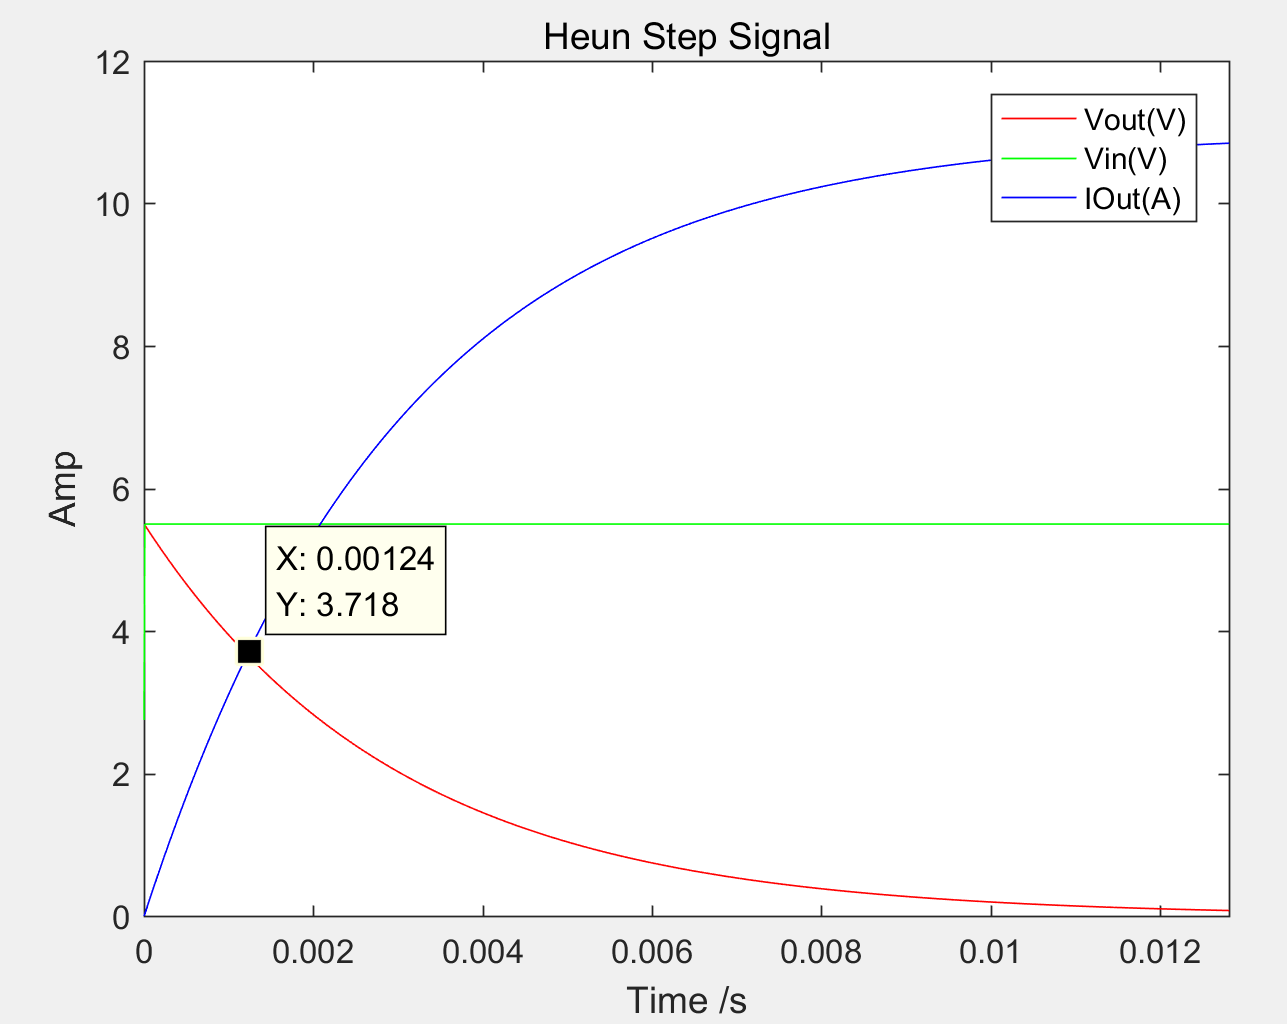
\includegraphics[width=\textwidth]{ex1/heun_step.PNG}
            \caption{Heun method}
      \end{subfigure}
      \caption{Step signal plots}
\label{fig:Step signal plots}
\end{figure}

In Figure \ref{fig:Step signal plots}, compared to the plots from Heun, Midpoint and Ralston method, we can see that the output is similar. Theoretically, at first, the voltage difference across the inductor is very high, so the current can barely pass through and $V_{out} = V_{in}$. From the plot, we can see $I_{out}$ is $0$ when $t = 0$. Then, due to the characteristics of the inductor, the voltage across the inductor decreases, so the current can pass through increasingly. Hence $V_{out}$ decreases and $I_{out}$ increases. By keeping Vin constant and equal to $5.5V$:

Mathematically, \[V_{Out} = V(e^{-RT/L})\] \[I_{Out} = V(1-e^{-RT/L})\]
when $t$ increases, $V_{out}$ decreases and $I_{out}$ increases. $V_{out}$ is constant here.

\begin{wrapfigure}{r}{0.4\textwidth}
\centering
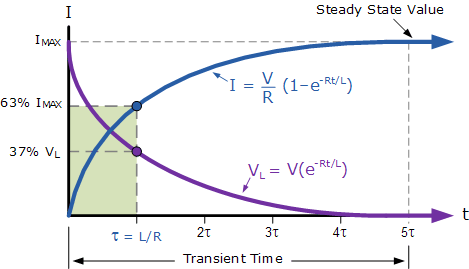
\includegraphics[width=0.38\textwidth]{ex1/heun_step_transient.png}
\caption{Transient graph}
\cite{lrtransient}
\end{wrapfigure}

The steady state value can be calculated by using
\[I_{max} = \frac{V_{in}}{R}\] the value is $\frac{5.5}{0.5} = 11A$.\par
\vspace{5mm}

In Figure \ref{fig:Step signal plots}, we can see that the results of these three methods are very similar compared to the plot of the RL circuit transient.


\subsubsection{MATLAB codes}
\lstinputlisting[caption = heun.m]{ex1/heun.m}\
\lstinputlisting[caption = heun\_script.m]{ex1/heun_script.m}
\lstinputlisting[caption = midpoint.m]{ex1/midpoint.m}
\lstinputlisting[caption = midpoint\_script.m]{ex1/midpoint_script.m}
\lstinputlisting[caption = ralston.m]{ex1/ralston.m}
\lstinputlisting[caption = ralston\_script.m]{ex1/ralston_script.m}
\newpage
\subsection{Impulsive signal and decay}
In this exercise, the input signal is as follows:
\begin{equation}\label{Exp eqn 1}
V_{in} = \bar{V}_{in} exp{\frac{-t^{2}}{\tau }}
\end{equation}
Or
\begin{equation}\label{Exp eqn 2}
V_{in} = \bar{V}_{in} exp{\frac{-t}{\tau }}
\end{equation}

The following graphs show how the output changes as we change the input signal.\par

\begin{figure}[h]
      \centering
      \begin{subfigure}[b]{0.4\textwidth}
            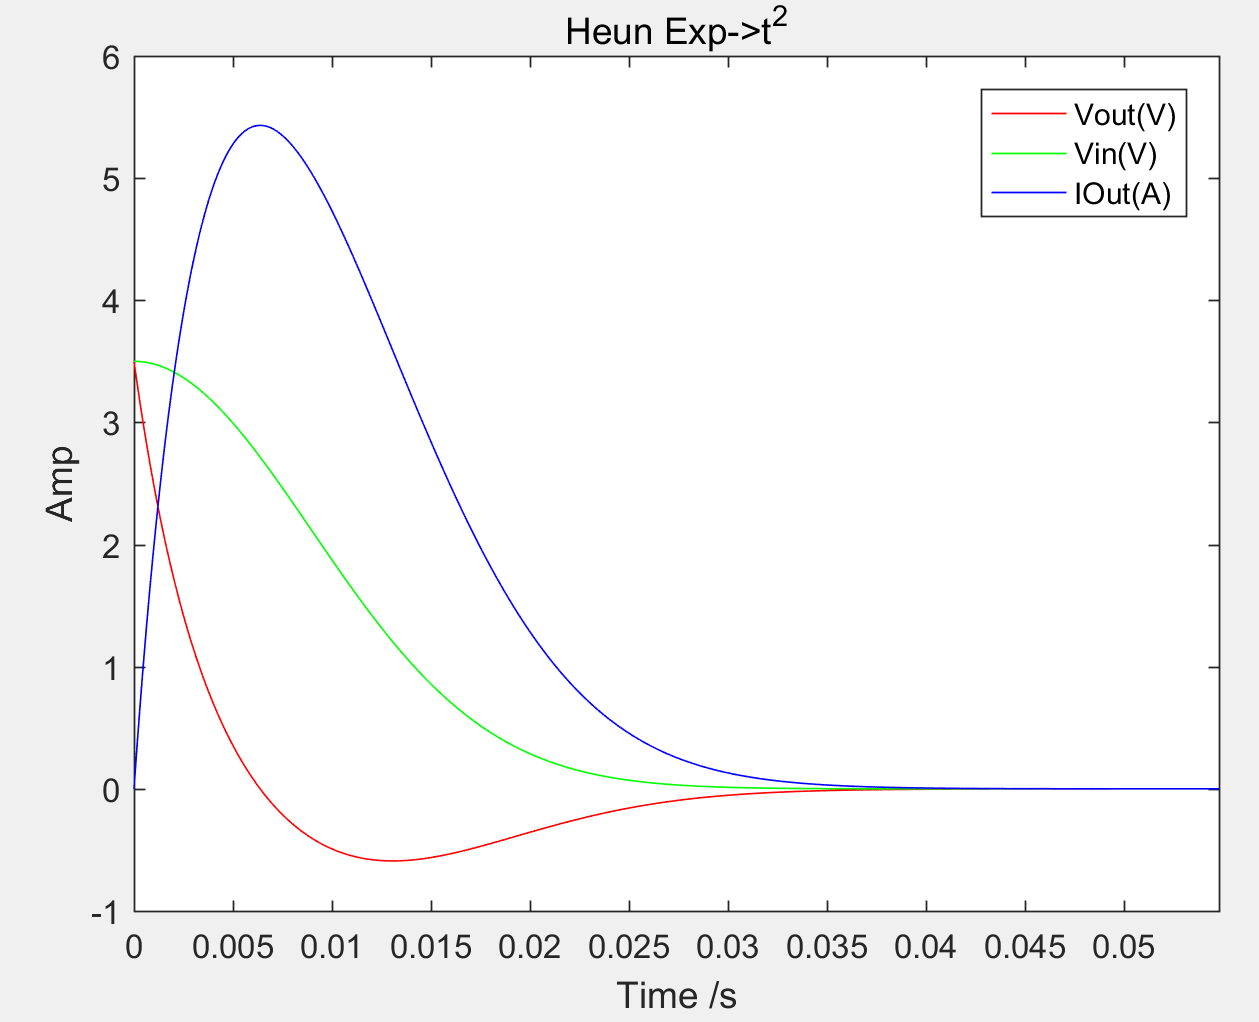
\includegraphics[width=\textwidth]{ex1/heun_exp_t_sqr.PNG}
            \caption{Equation 1}
      \end{subfigure}
      ~
      \begin{subfigure}[b]{0.4\textwidth}
            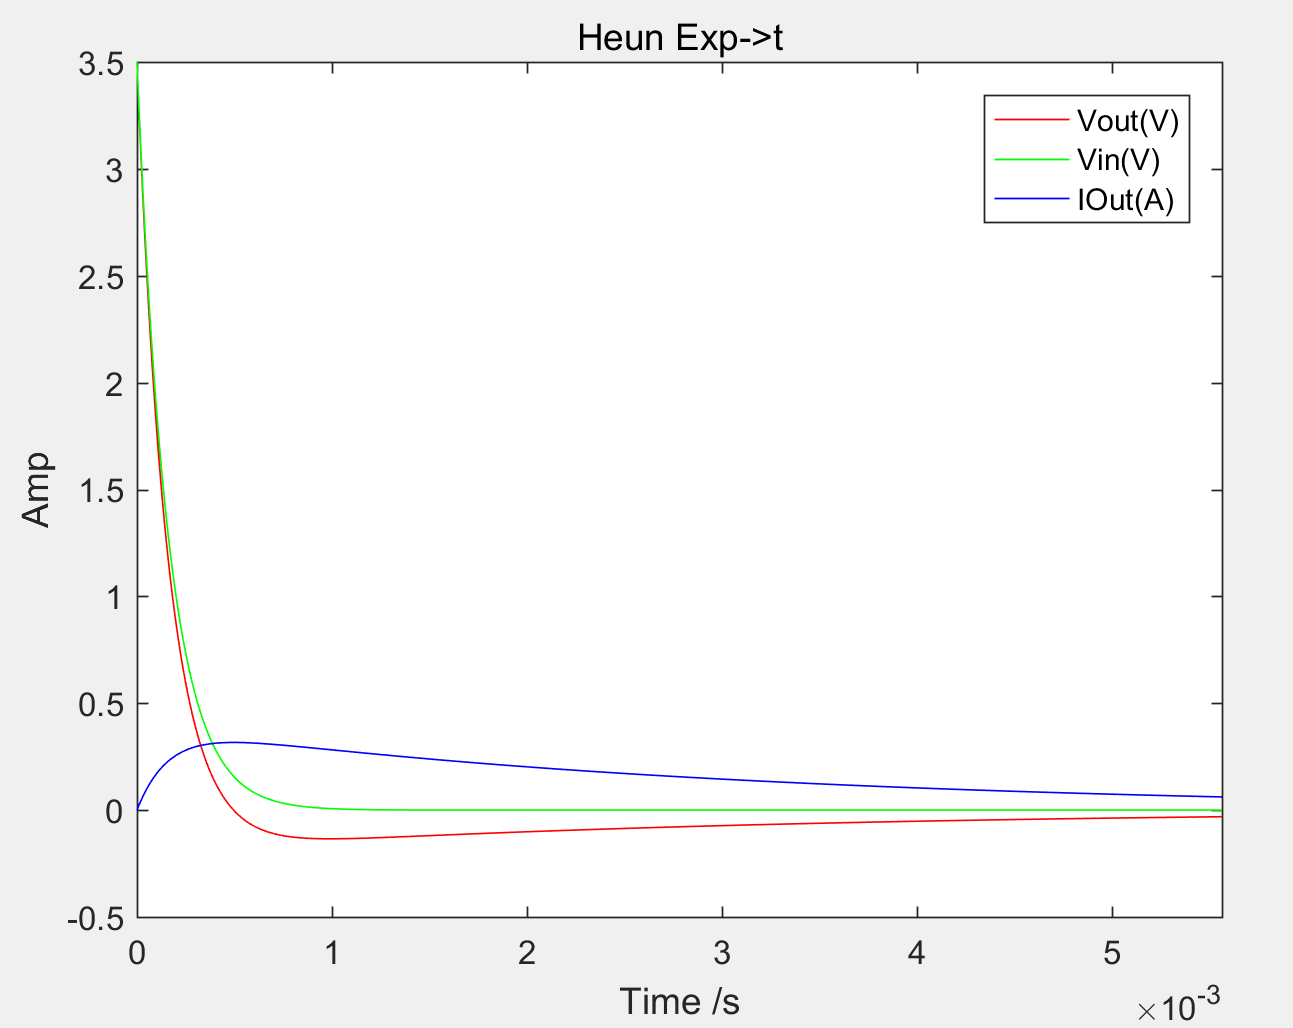
\includegraphics[width=\textwidth]{ex1/heun_exp_t.PNG}
            \caption{Equation 2}
      \end{subfigure}
      \caption{Heun's method}
\end{figure}

As we can see, the average value of the current out in equation (3) is much higher than in equation (4). \par
Mathematically, when we multiply the voltage in with the exponential, the output is similar to the plot above.\par
Theoretically, equation (3) voltage changes more slowly than for equation (4). At first, the inductor acts like an open circuit, so it takes most of the voltage. When voltage-in decreases steadily, the inductor becomes more like a coil of wire with zero/low resistance, so the voltage across it decreases steadily. As the decrement is slow in equation (3), most of the current will pass through, hence we got a higher value of current-out in Figure 5.a.

\newpage
The following plots using Midpoint and Ralston methods:

\begin{figure}[h]
      \centering
      \begin{subfigure}[b]{0.4\textwidth}
            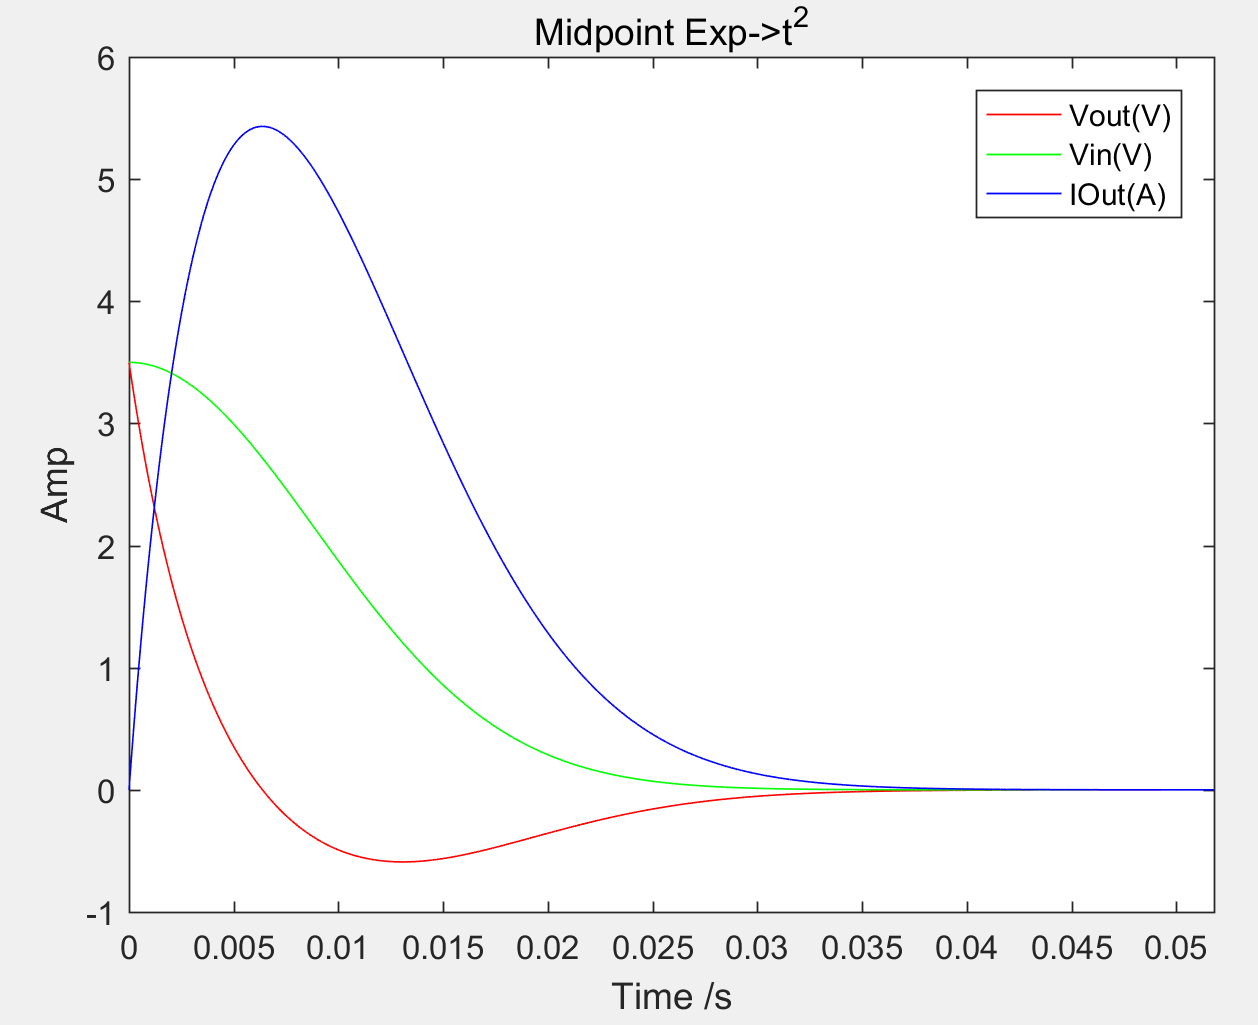
\includegraphics[width=\textwidth]{ex1/Midpoint_t_sqr.PNG}
            \caption{Equation 1}
      \end{subfigure}
      ~
      \begin{subfigure}[b]{0.4\textwidth}
            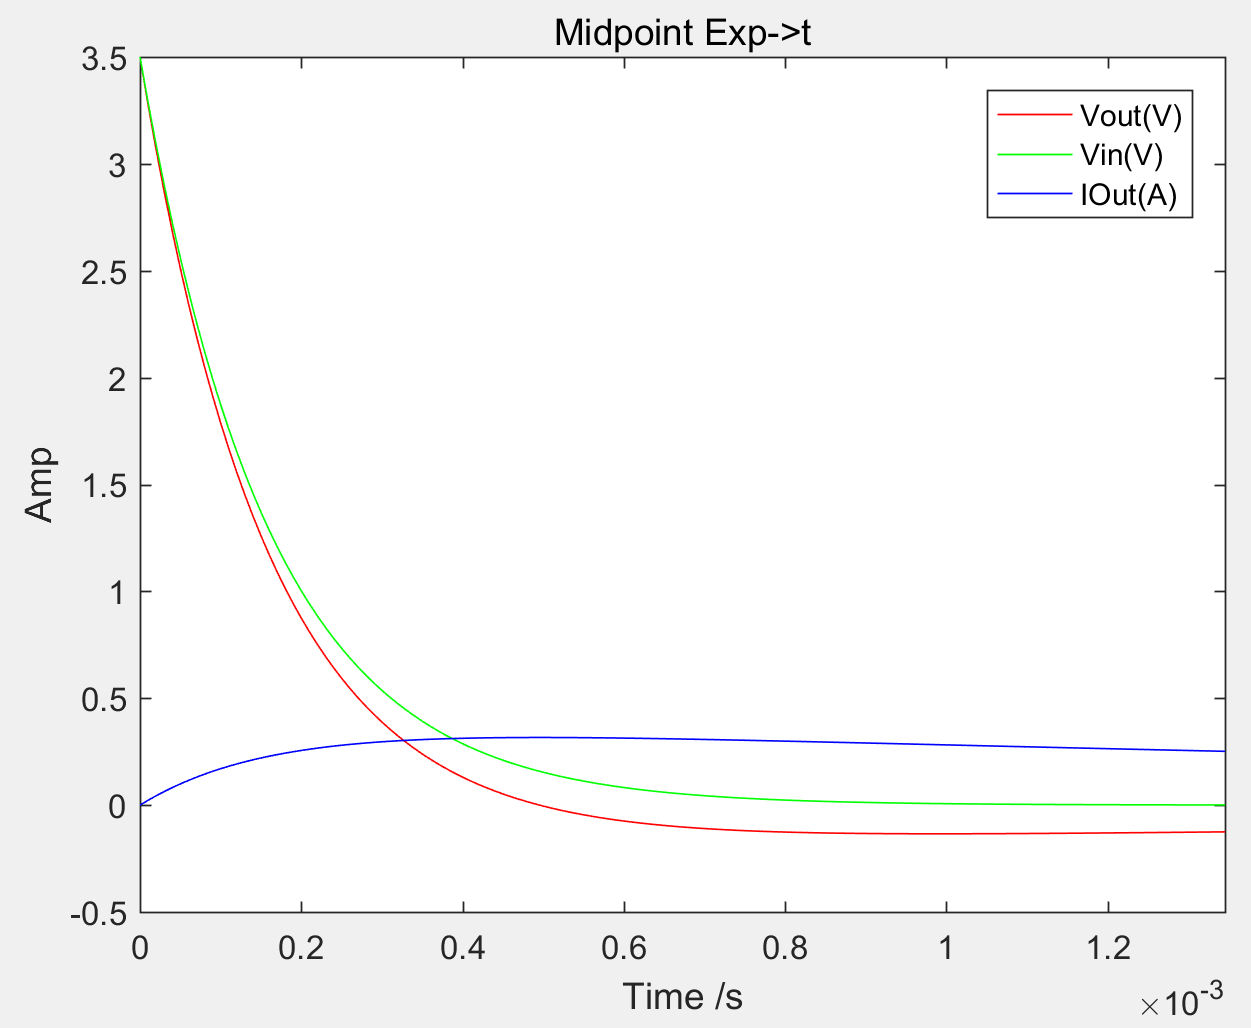
\includegraphics[width=\textwidth]{ex1/Midpoint_t.PNG}
            \caption{Equation 2}
      \end{subfigure}
      \caption{Midpoint method}
\end{figure}

\begin{figure}[h]
      \centering
      \begin{subfigure}[b]{0.4\textwidth}
            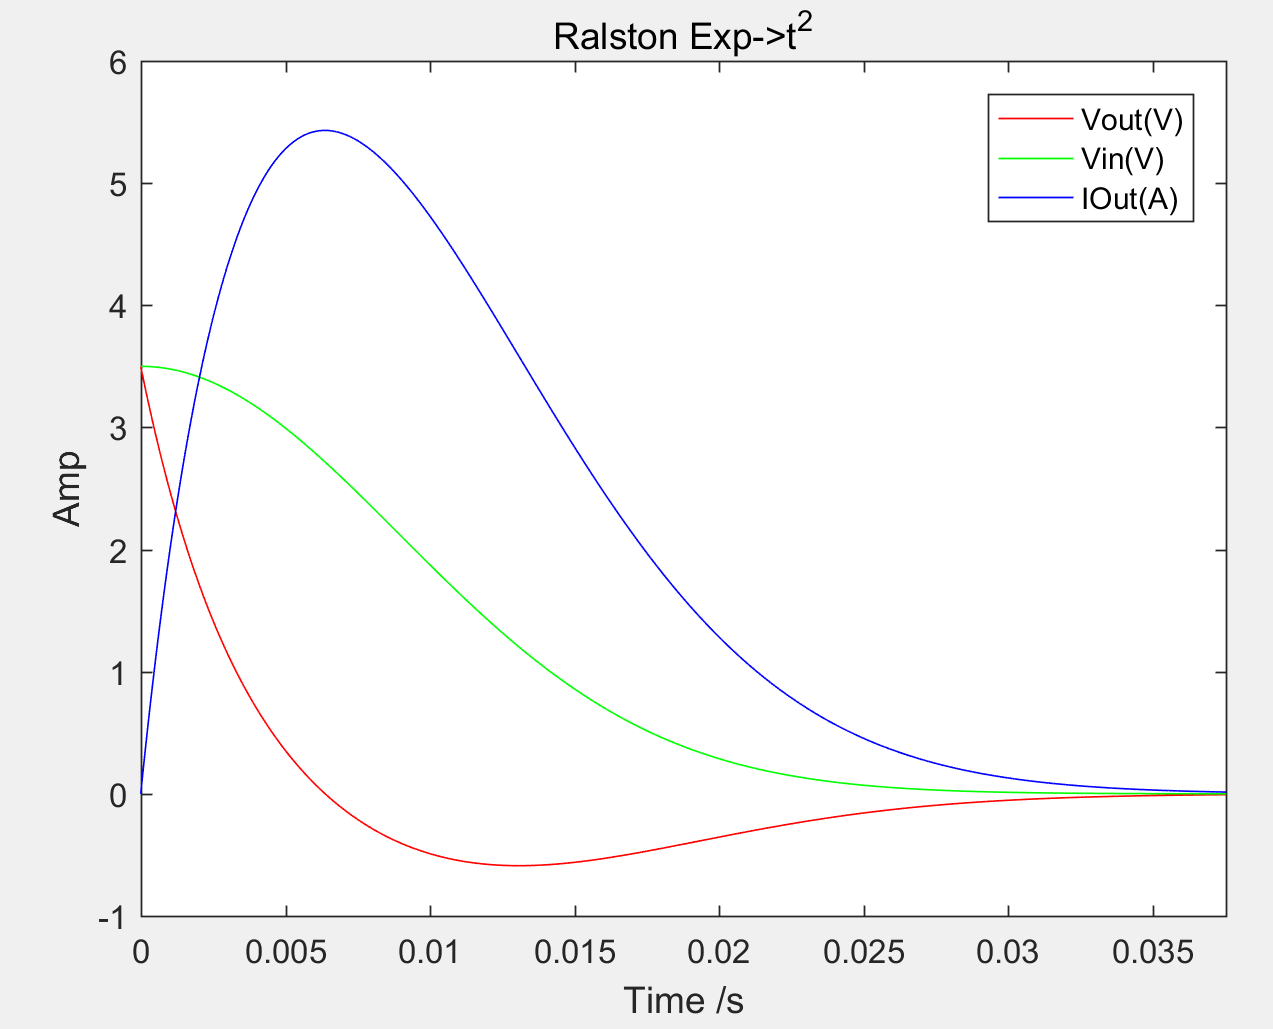
\includegraphics[width=\textwidth]{ex1/ralston_t_sqr.PNG}
            \caption{Equation 1}
      \end{subfigure}
      ~
      \begin{subfigure}[b]{0.4\textwidth}
            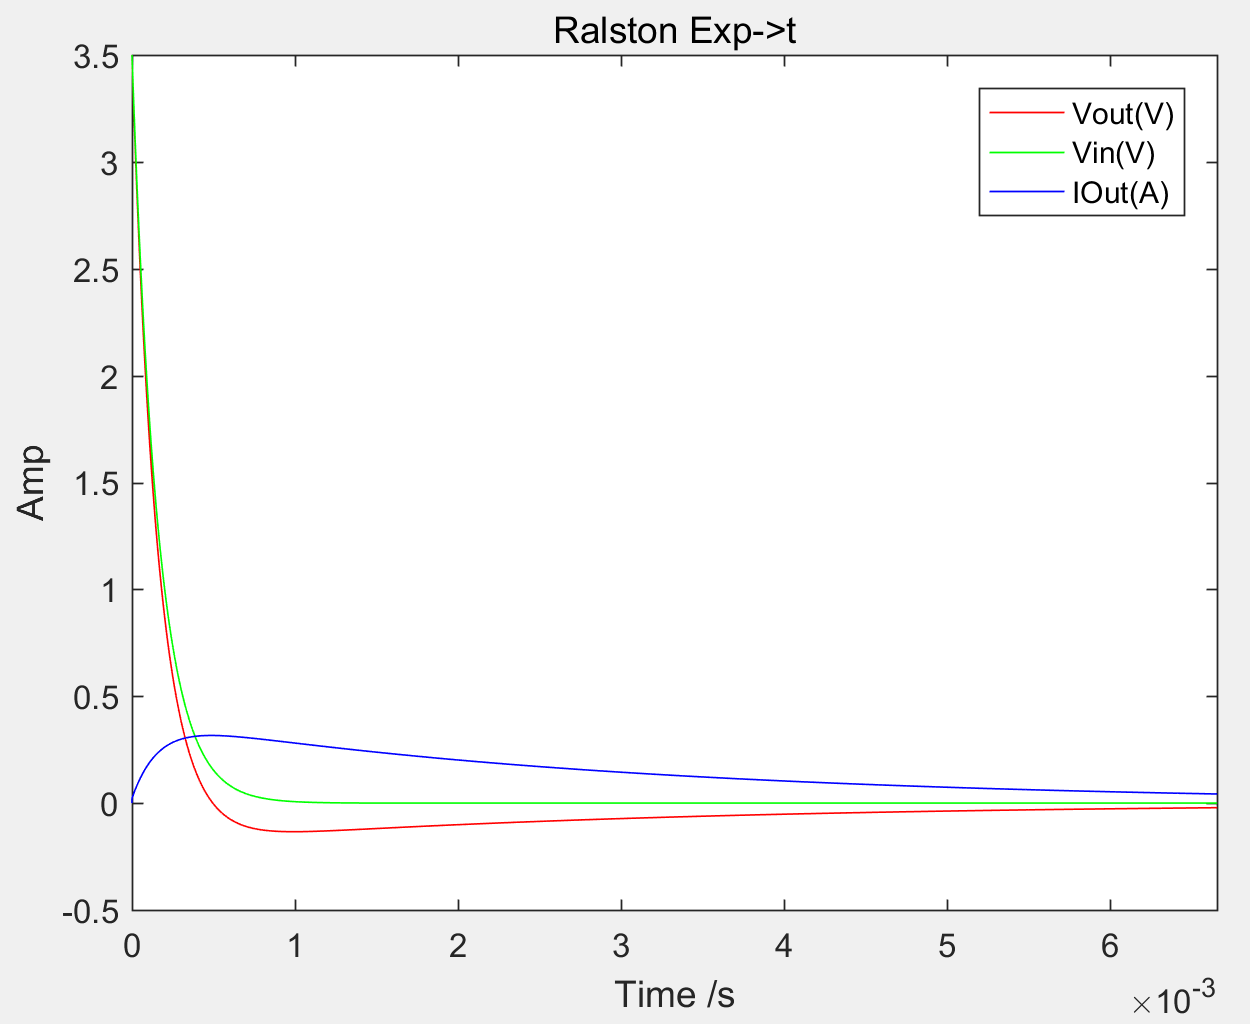
\includegraphics[width=\textwidth]{ex1/ralston_t.PNG}
            \caption{Equation 2}
      \end{subfigure}
      \caption{Ralston method}
\end{figure}

Compare to these results, we can see that the simulations are similar. \par


\newpage
\subsubsection{MATLAB codes}
\lstinputlisting[caption = heun.m]{ex1/heun.m}\par
\lstinputlisting[caption = heun script.m]{ex1/heun_script_q2.m}
\lstinputlisting[caption = midpoint.m]{ex1/midpoint.m}\par
\lstinputlisting[caption = midpoint script.m]{ex1/midpoint_script_q2.m}
\lstinputlisting[caption = ralston.m]{ex1/ralston.m}\par
\lstinputlisting[caption = ralston script.m]{ex1/ralston_script_q2.m}
\newpage
\subsection{Sine Saw-tooth and square input}
\indent Question:\par
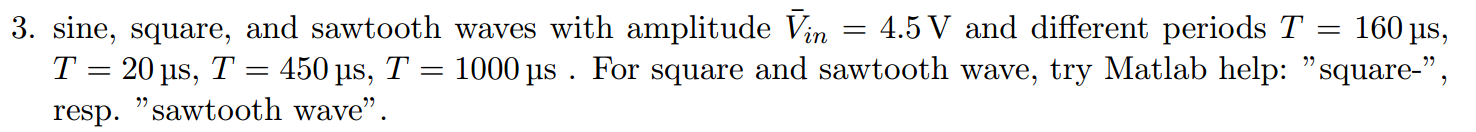
\includegraphics[width=\textwidth]{ex1/q3.PNG}

\subsubsection{Sine input}
In this part, we input a sine wave into the circuit(Heun's Method).
As we can see, except for period = 450, there is no phase shift in Vout:
\begin{figure}[h]
      \centering
      \begin{subfigure}[b]{0.4\textwidth}
            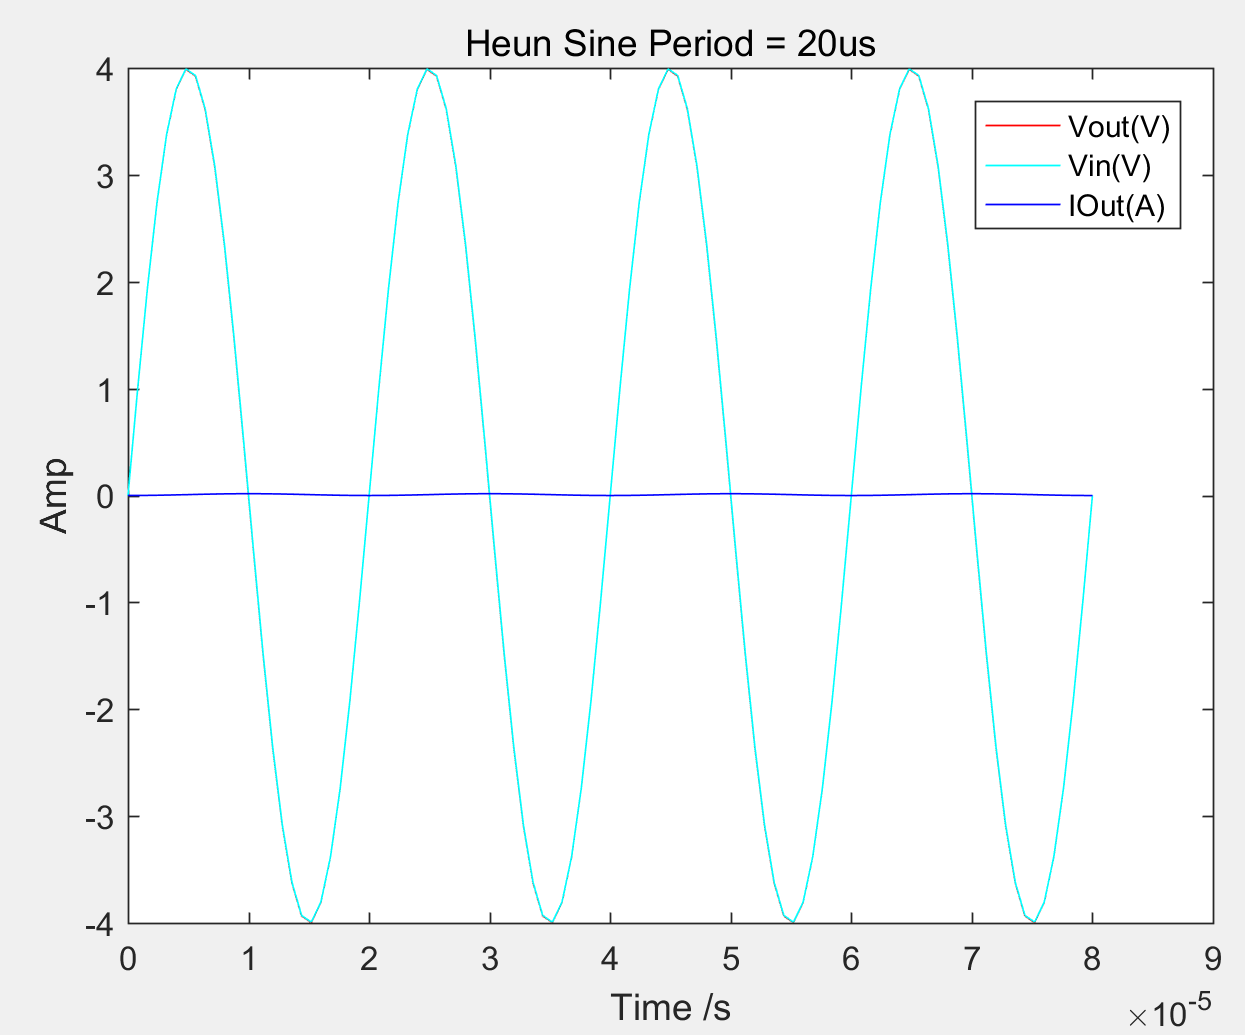
\includegraphics[width=\textwidth]{ex1/heun_sin_20.PNG}
            \caption{Heun sin T=20}
      \end{subfigure}
      ~
      \begin{subfigure}[b]{0.4\textwidth}
            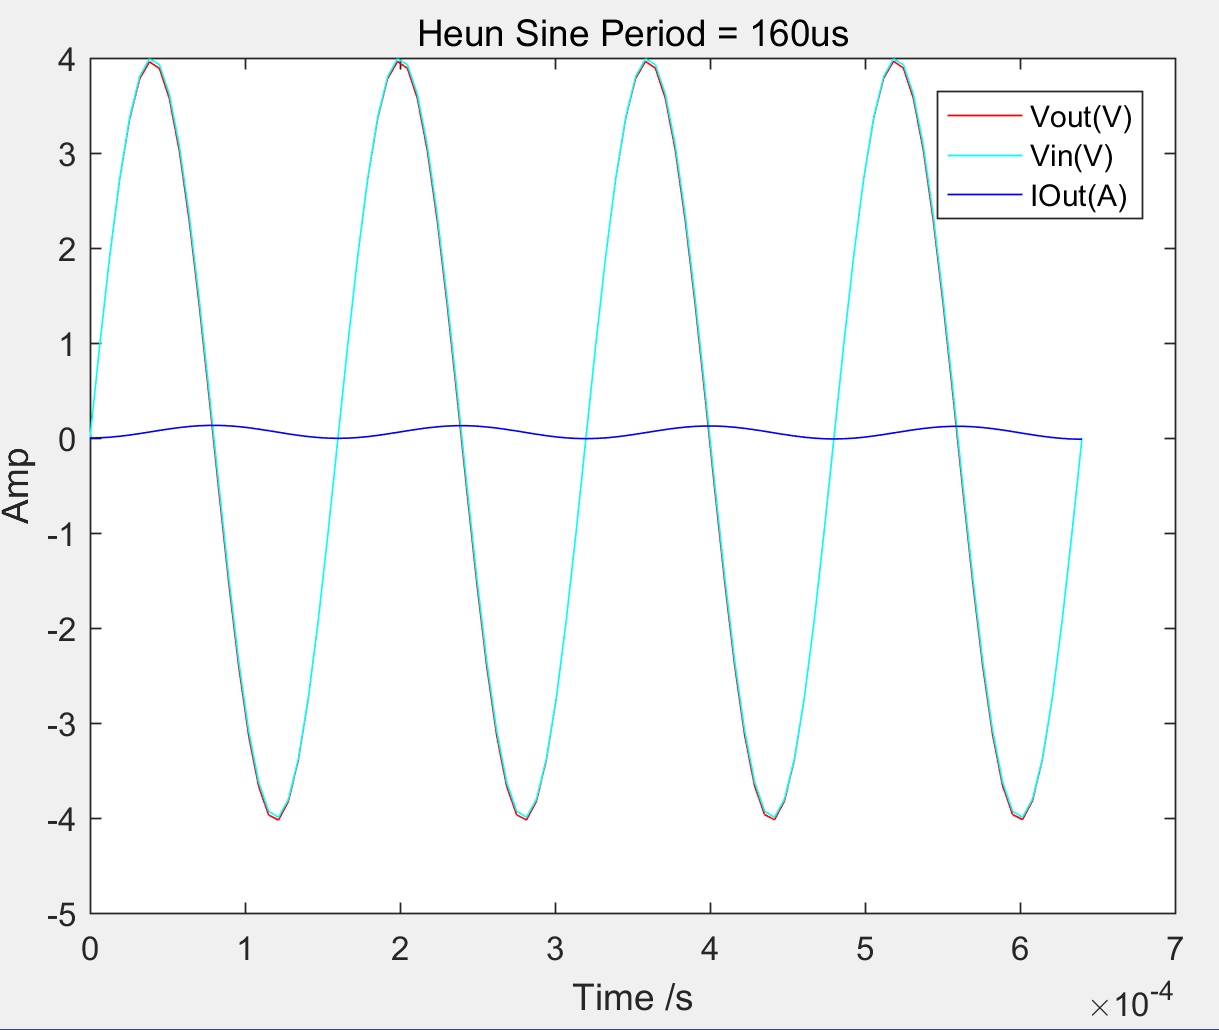
\includegraphics[width=\textwidth]{ex1/heun_sin_160.PNG}
            \caption{Heun sin T=160}
      \end{subfigure}
       ~
      \begin{subfigure}[b]{0.4\textwidth}
            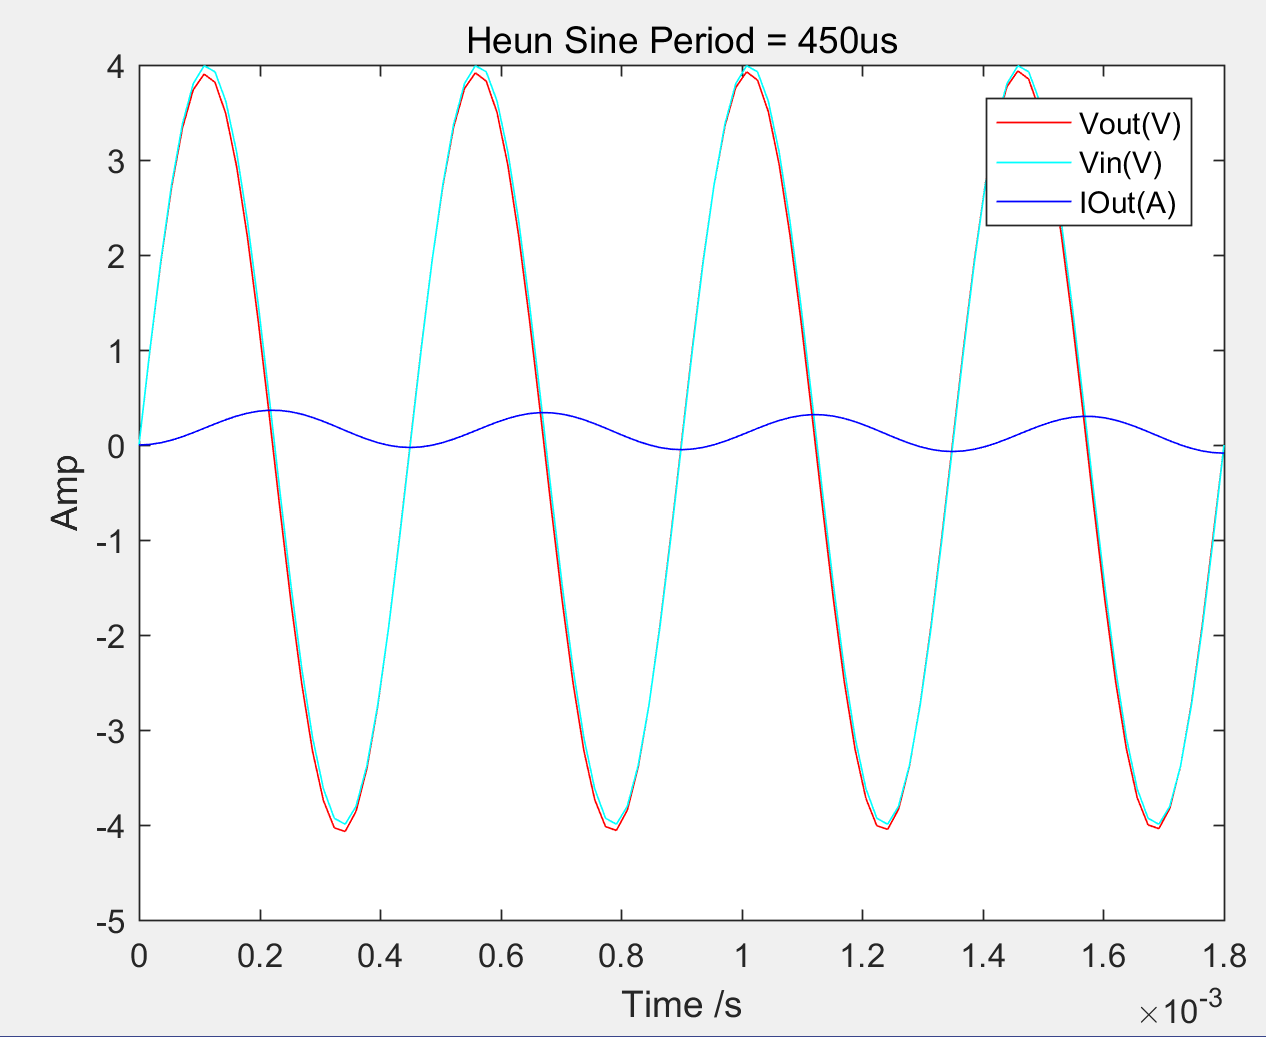
\includegraphics[width=\textwidth]{ex1/heun_sin_450.PNG}
            \caption{Heun sin T=450}
      \end{subfigure}
       ~
      \begin{subfigure}[b]{0.4\textwidth}
            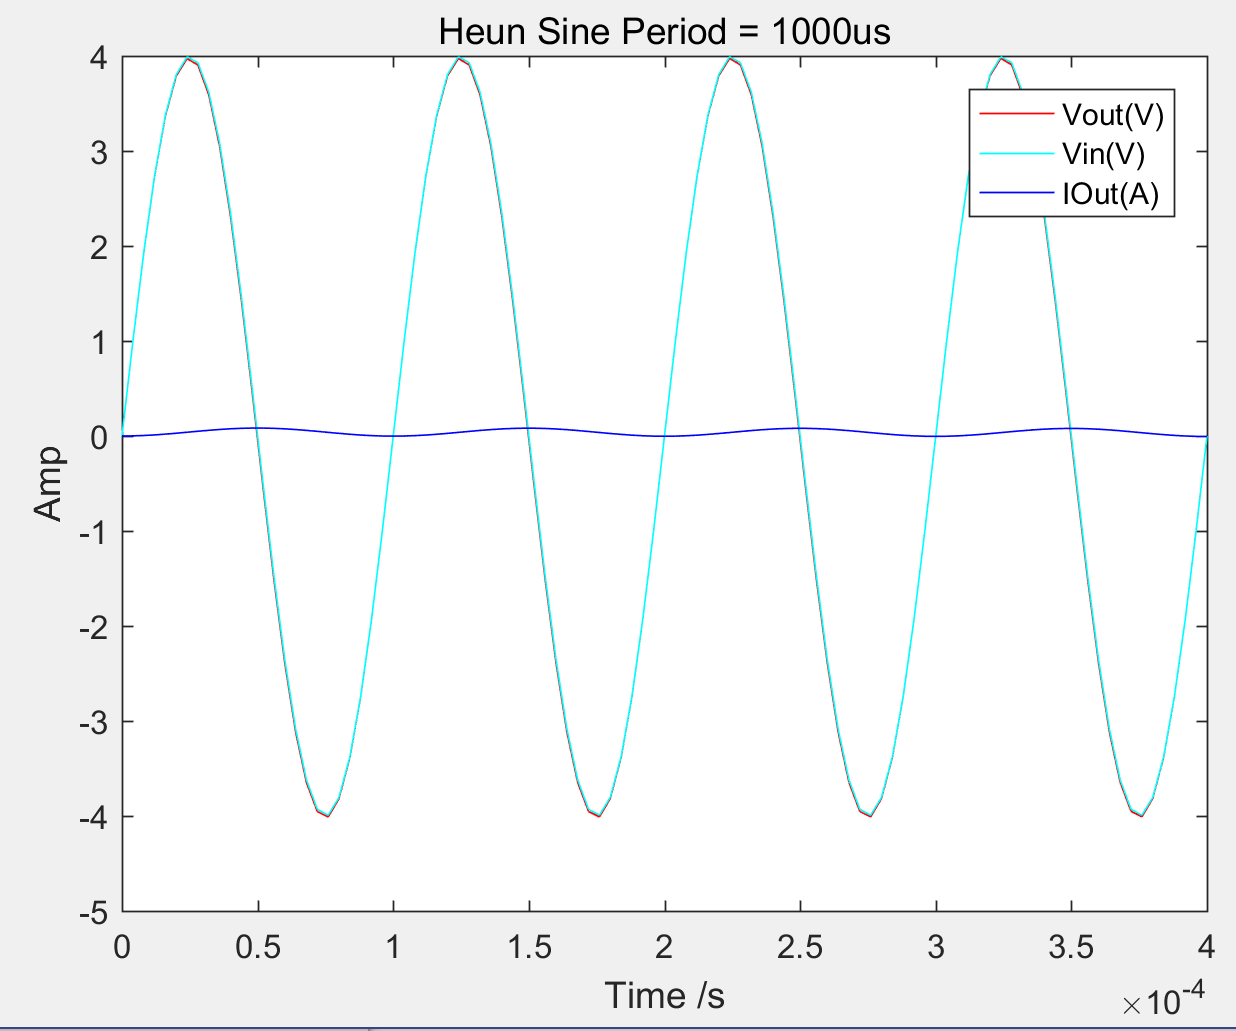
\includegraphics[width=\textwidth]{ex1/heun_sin_1000.PNG}
            \caption{Heun sin T=1000}
      \end{subfigure}
      \caption{Heun's method}
\end{figure}

\newpage
And the following plots are for Midpoint and Ralston methods:
\begin{figure}[h]
      \centering
      \begin{subfigure}[b]{0.4\textwidth}
            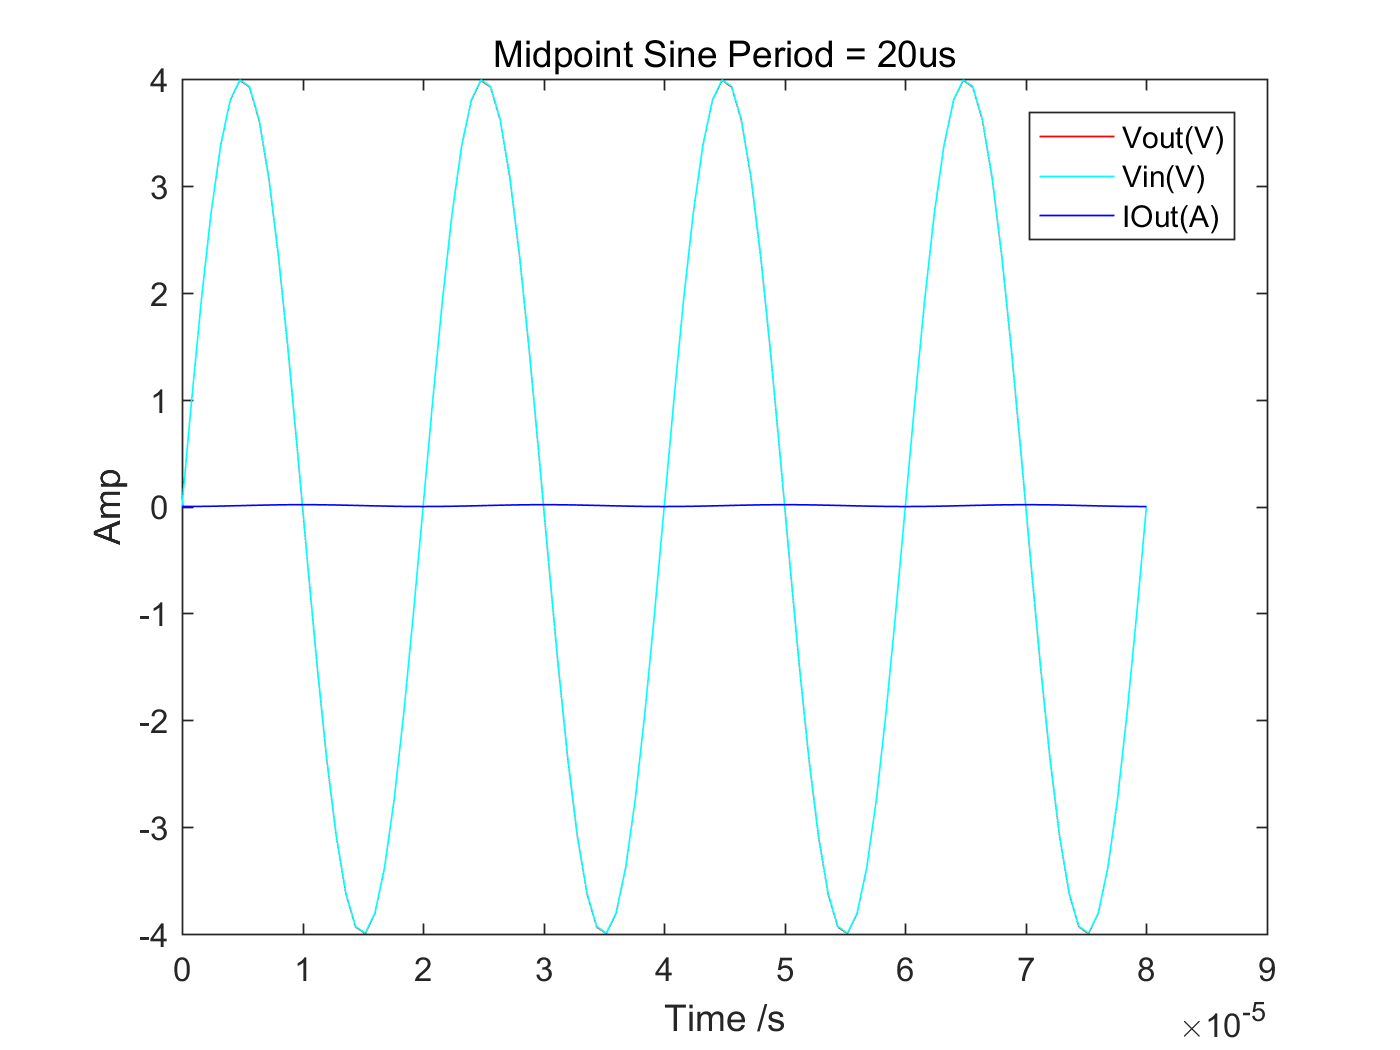
\includegraphics[width=\textwidth]{ex1/midpoint_mid_sin_20.png}
            \caption{Midpoint sin T=20}
      \end{subfigure}
      ~
      \begin{subfigure}[b]{0.4\textwidth}
            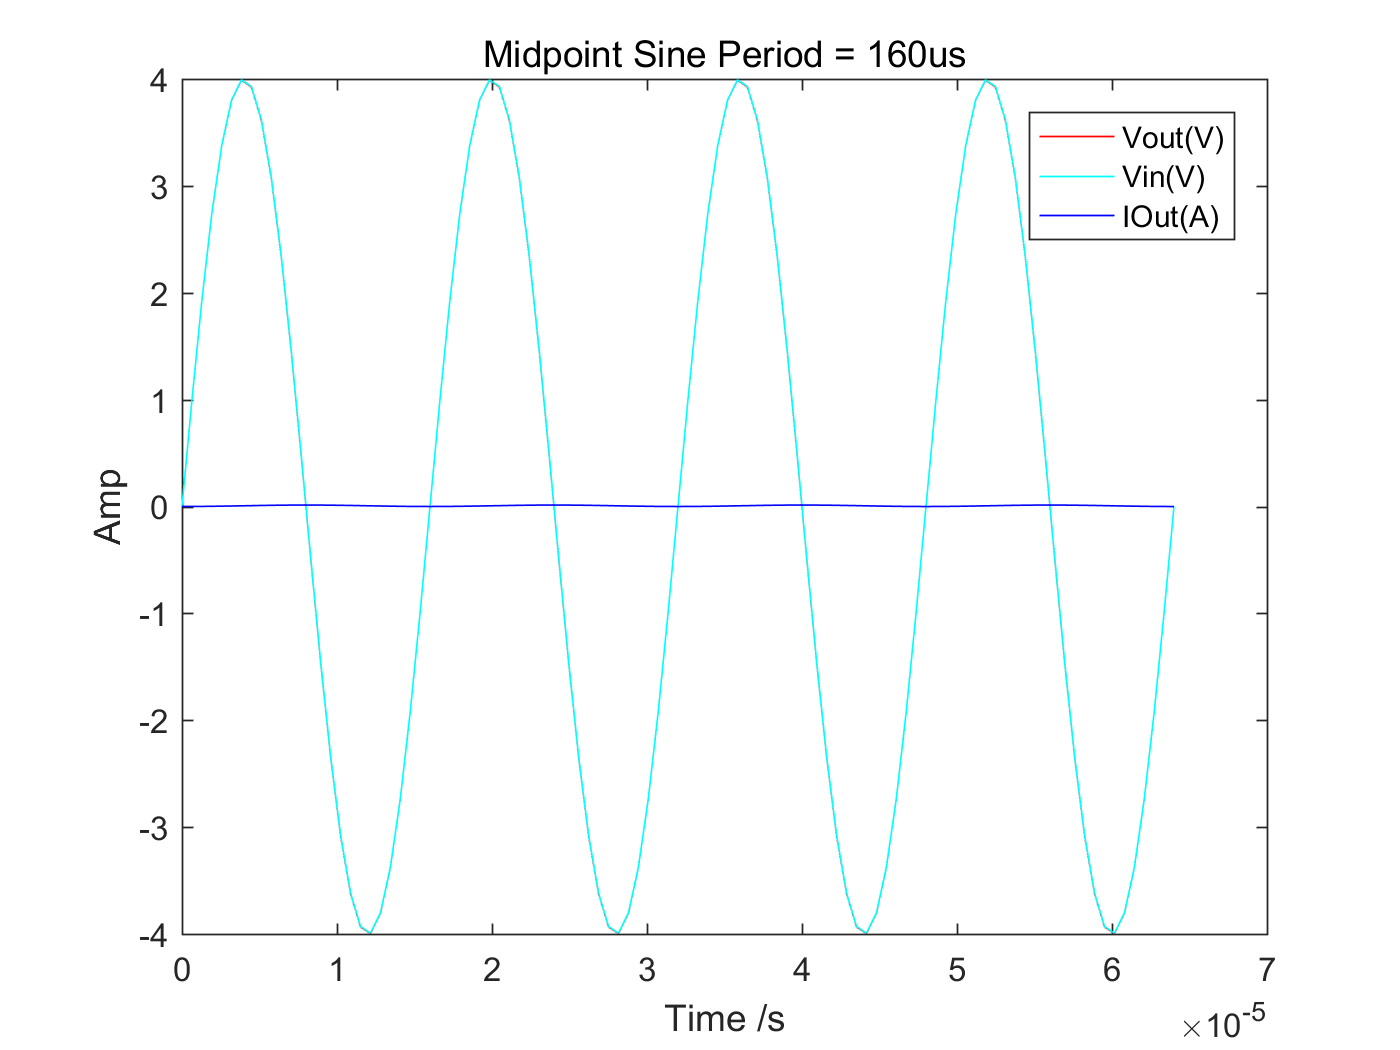
\includegraphics[width=\textwidth]{ex1/midpoint_mid_sin_160.png}
            \caption{Midpoint sin T=160}
      \end{subfigure}
       ~
      \begin{subfigure}[b]{0.4\textwidth}
            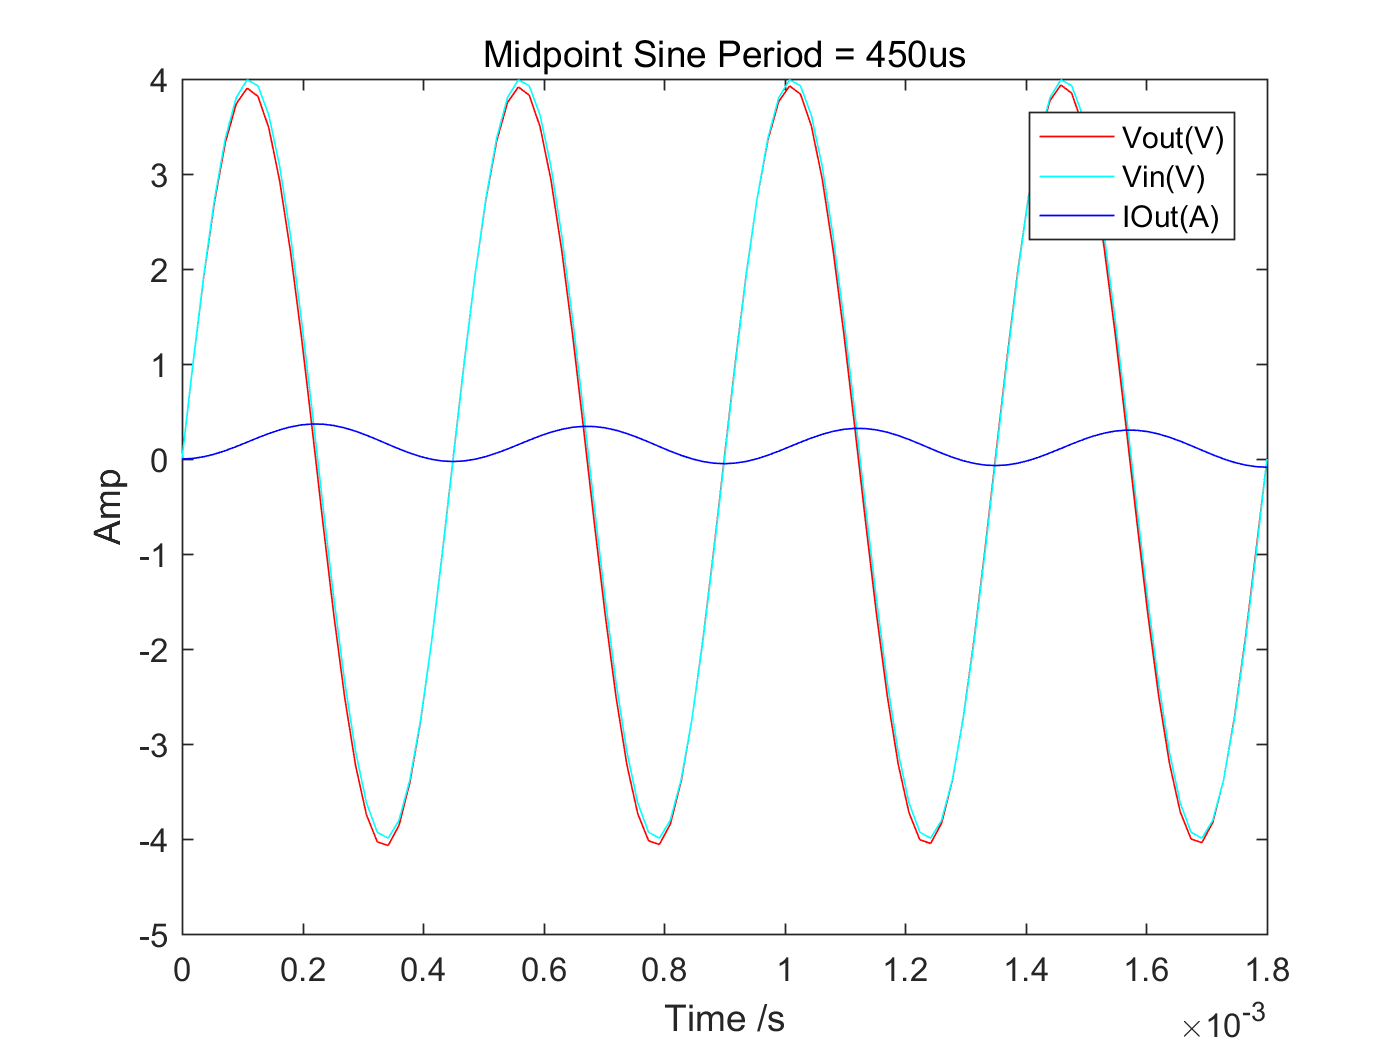
\includegraphics[width=\textwidth]{ex1/midpoint_mid_sin_450.png}
            \caption{Midpoint sin T=450}
      \end{subfigure}
       ~
      \begin{subfigure}[b]{0.4\textwidth}
            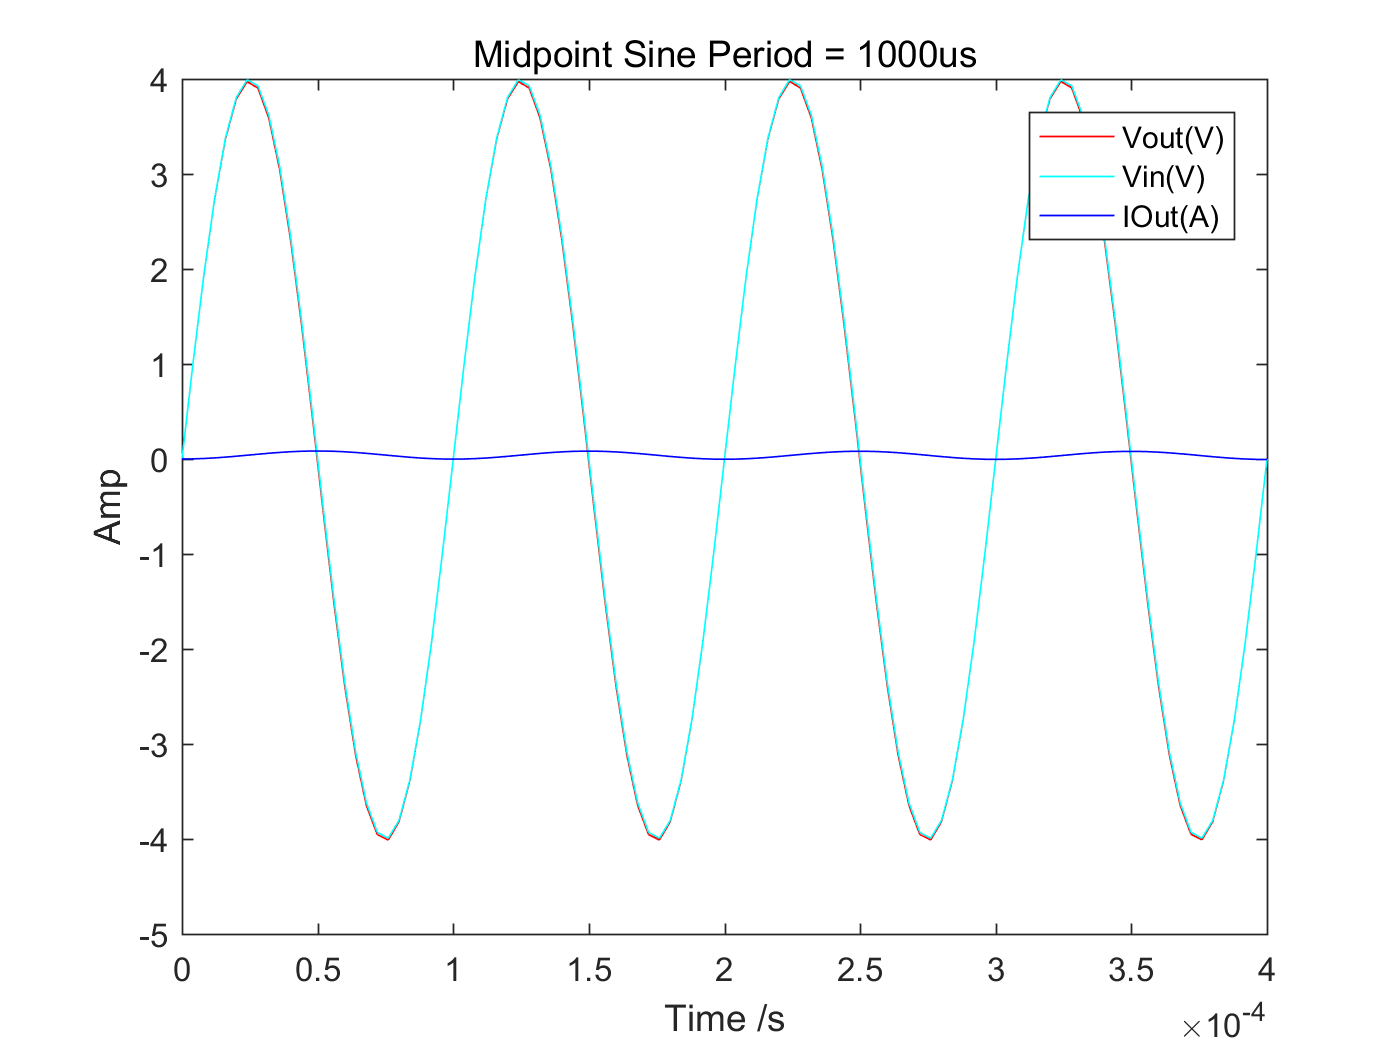
\includegraphics[width=\textwidth]{ex1/midpoint_mid_sin_1000.png}
            \caption{Midpoint sin T=1000}
      \end{subfigure}
      \caption{Midpoint method}
\end{figure}
\newpage
\begin{figure}[h]
      \centering
      \begin{subfigure}[b]{0.4\textwidth}
            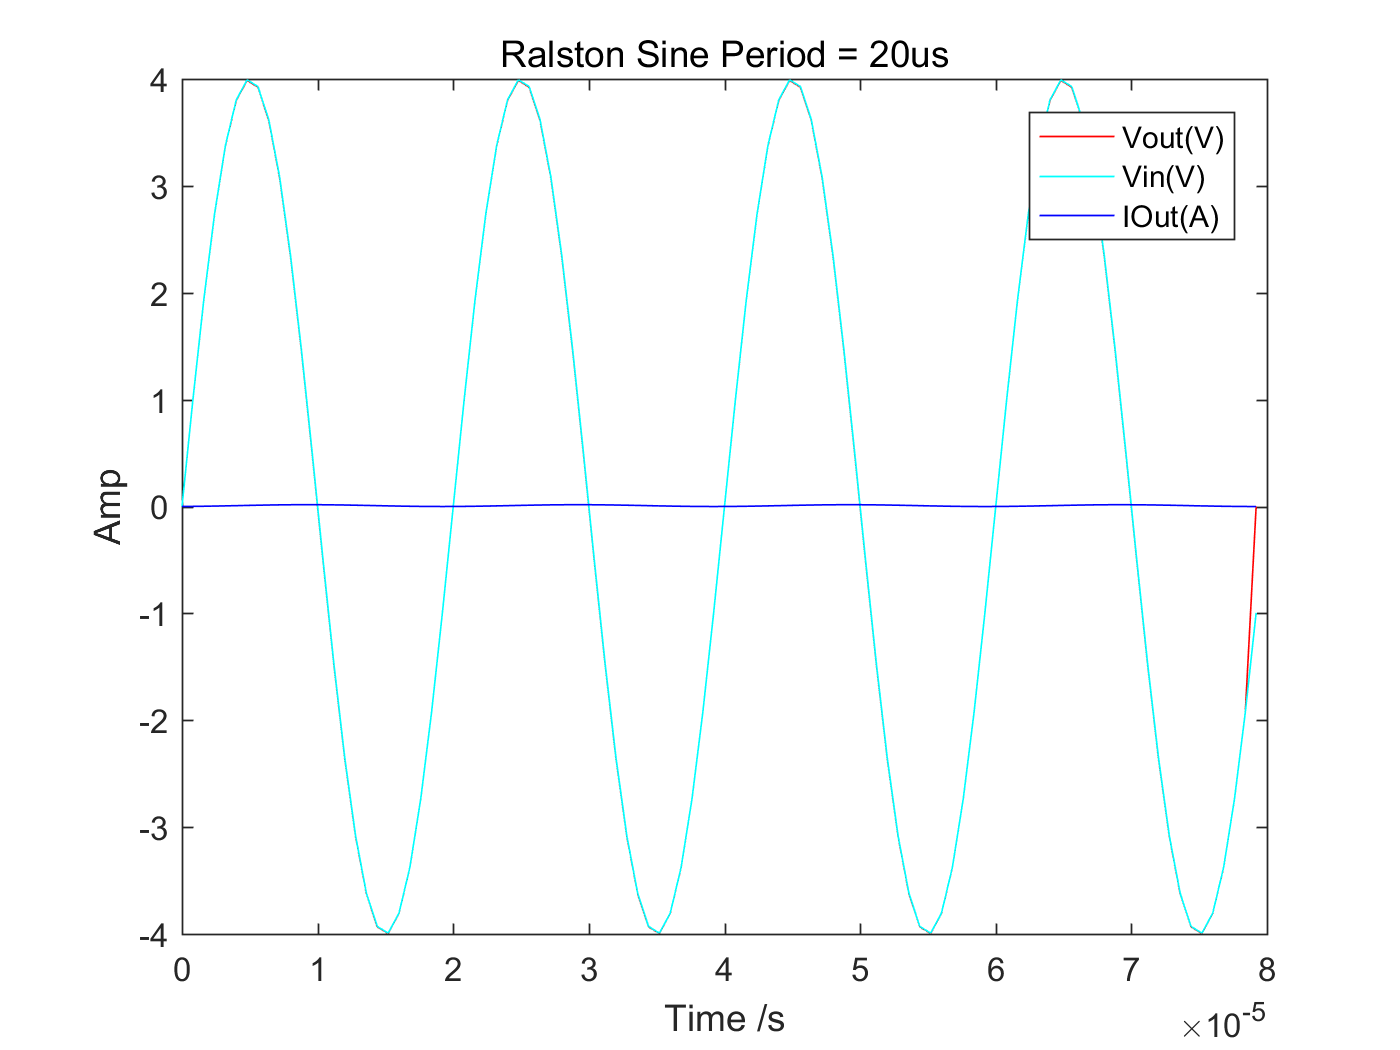
\includegraphics[width=\textwidth]{ex1/ralston_t_equal_to_20.png}
            \caption{Ralston sin T=20}
      \end{subfigure}
      ~
      \begin{subfigure}[b]{0.4\textwidth}
            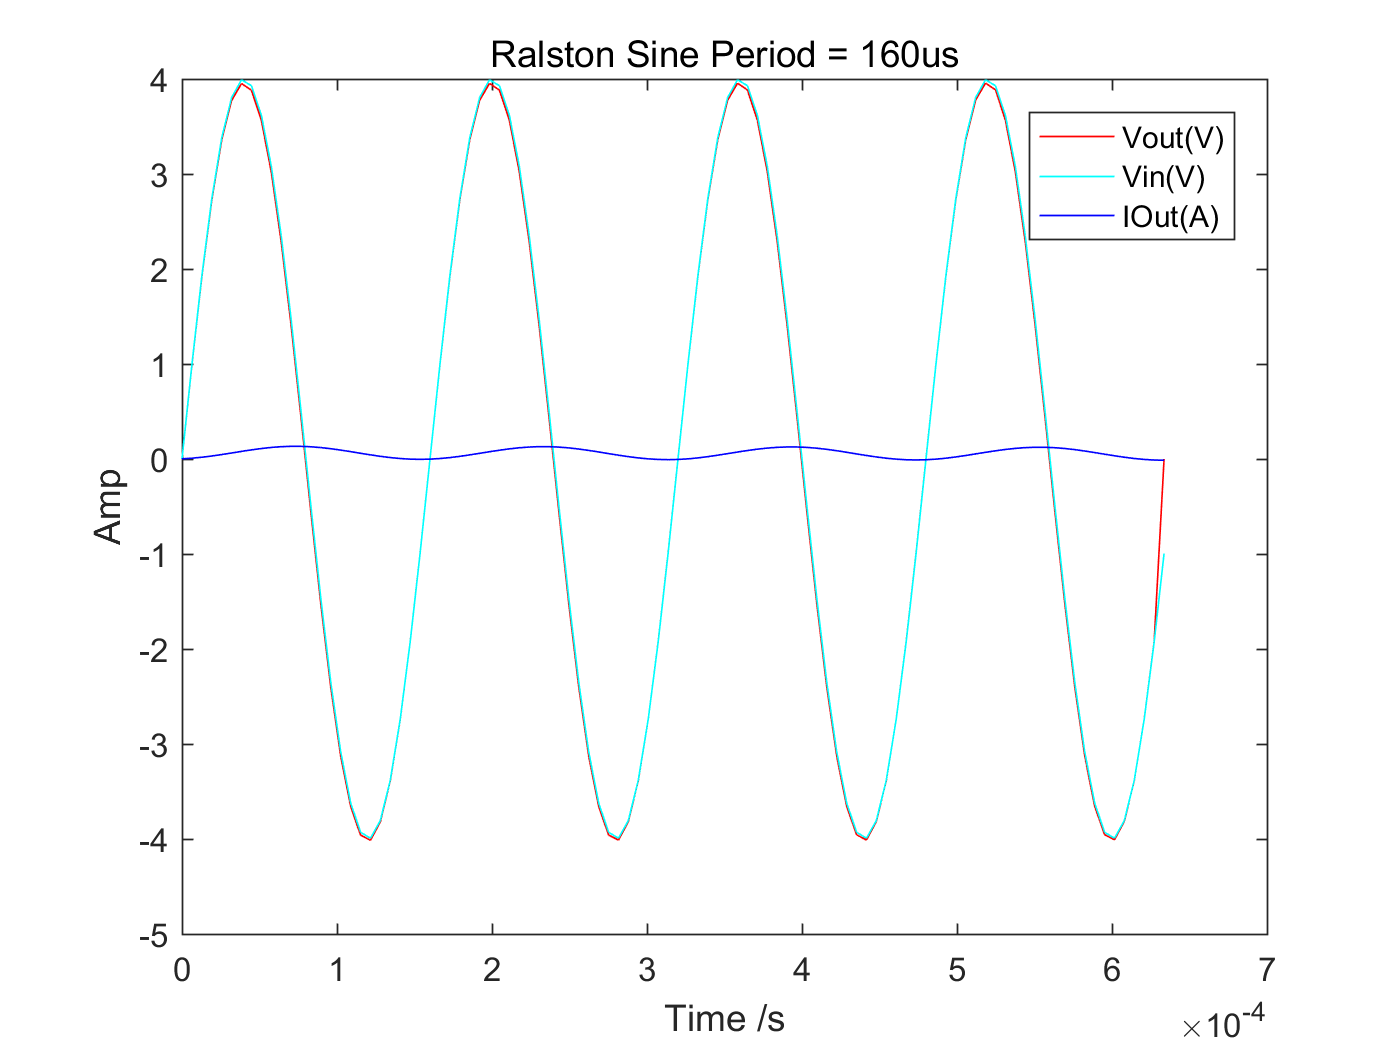
\includegraphics[width=\textwidth]{ex1/ralston_t_equal_to_160.png}
            \caption{Ralston sin T=160}
      \end{subfigure}
       ~
      \begin{subfigure}[b]{0.4\textwidth}
            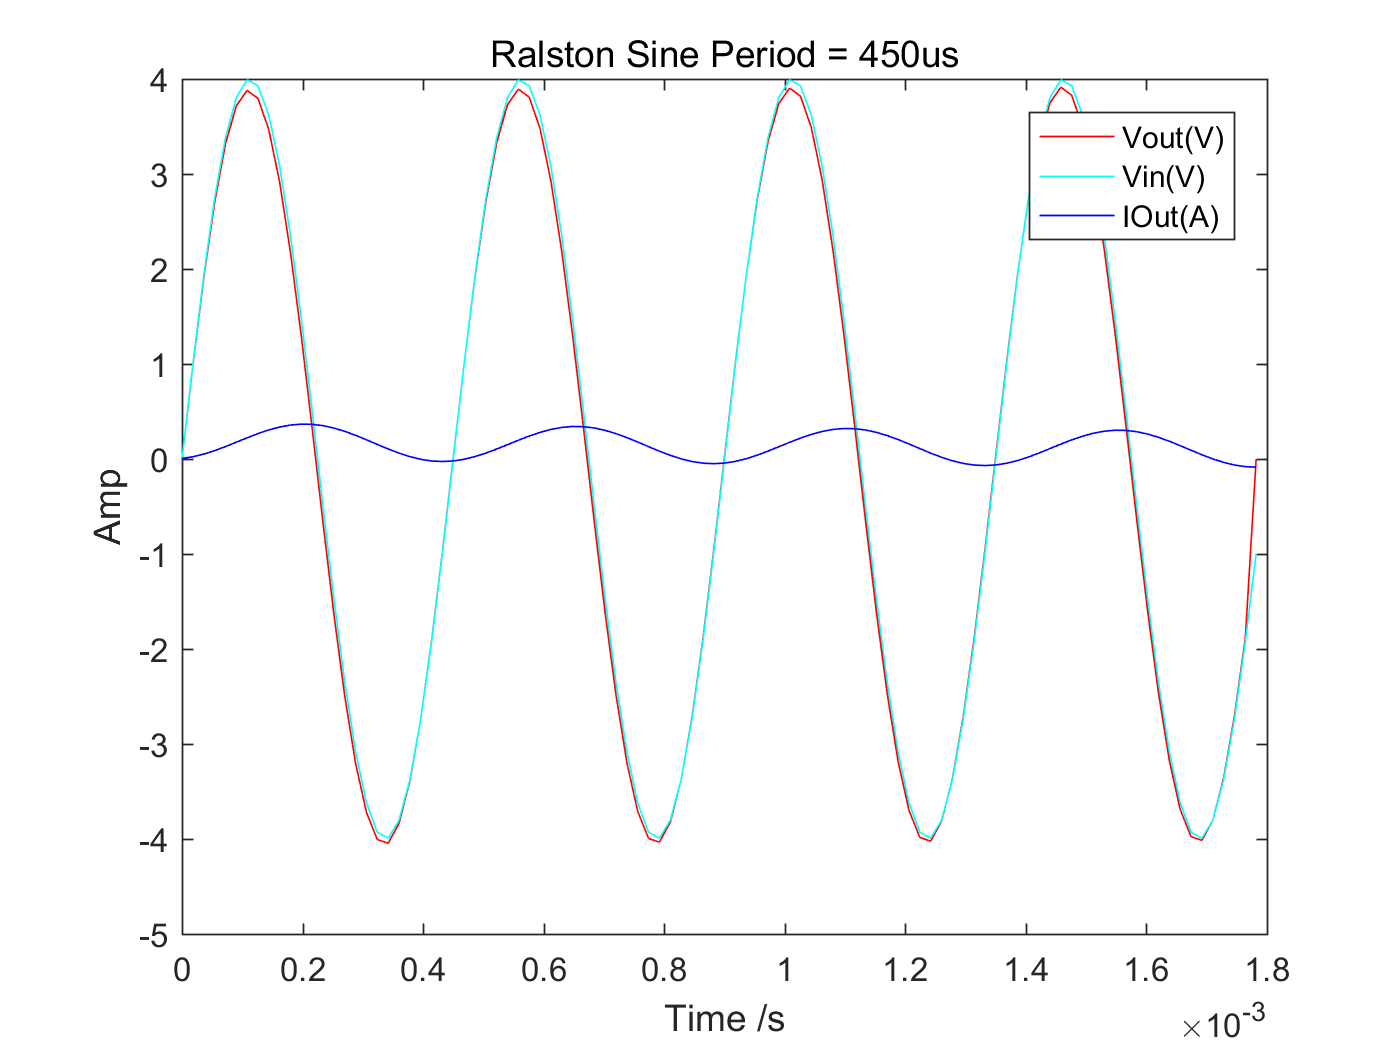
\includegraphics[width=\textwidth]{ex1/ralston_t_equal_to_450.png}
            \caption{Ralston sin T=450}
      \end{subfigure}
       ~
      \begin{subfigure}[b]{0.4\textwidth}
            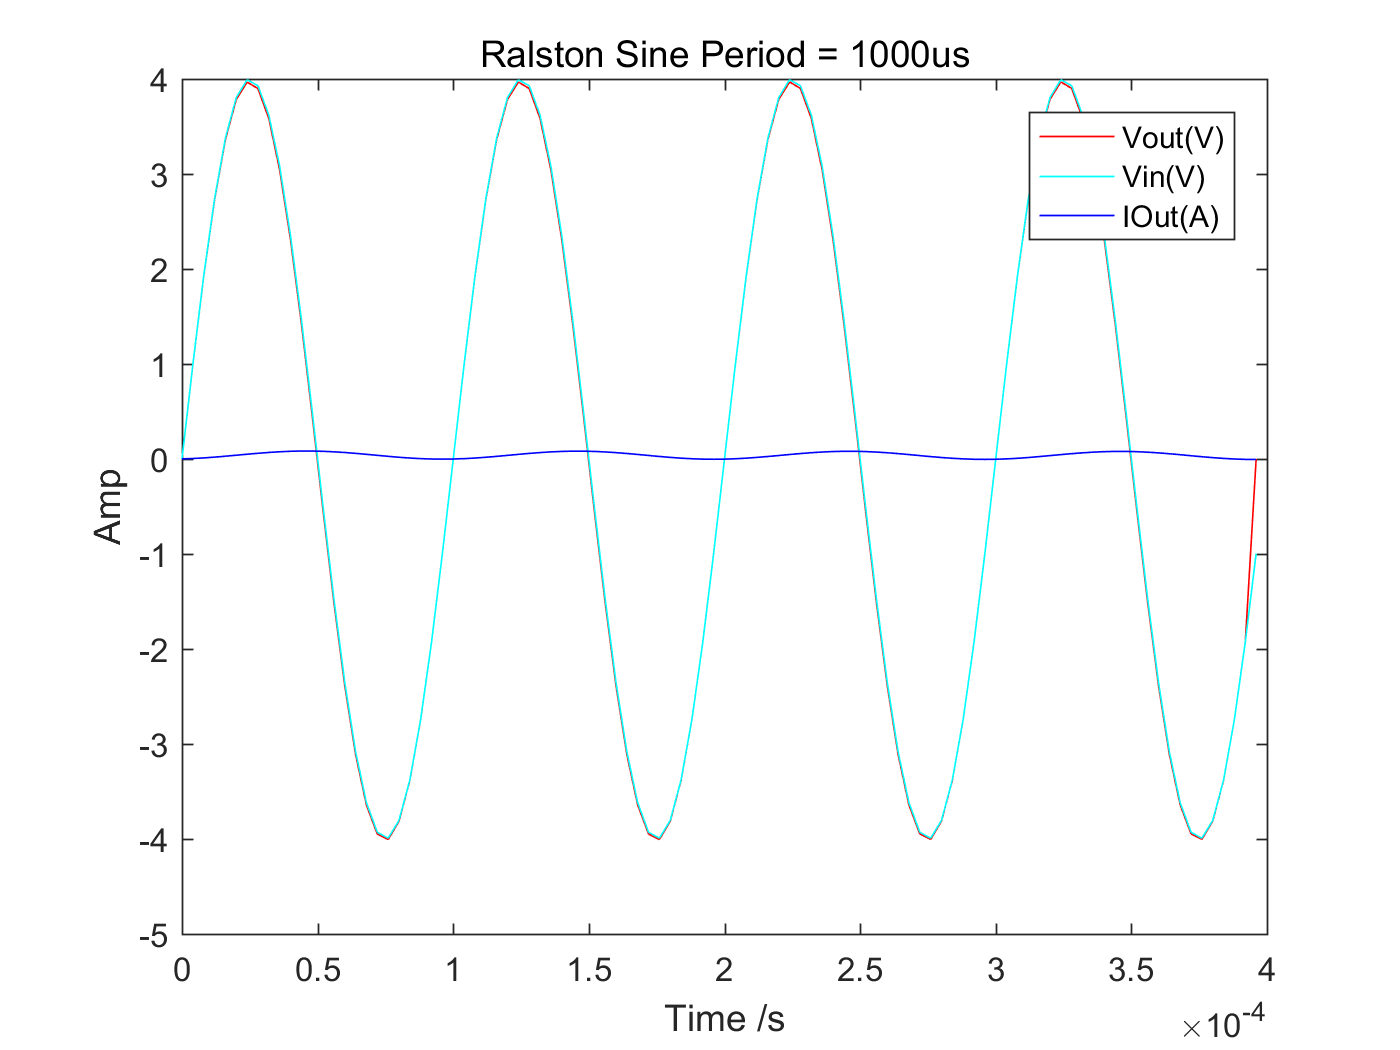
\includegraphics[width=\textwidth]{ex1/ralston_t_equal_to_1000.png}
            \caption{Ralston sin T=1000}
      \end{subfigure}
      \caption{Ralston method}
\end{figure}


\begin{equation}\label{inductor}
v=L\frac{di}{dt}
\end{equation} 
In conclusion, for an ideal inductor, it has negligible resistance and capacitance. Hence, the voltage across the inductor is only due to the magnetic field around itself and the electromagnetic induction due to Faraday's law. \par
As a consequence of equation (5), we can see that for the inductor, its voltage and current are out of phase. When the input is a sinusoidal sine wave, its derivative is cosine, so when current changes at its most regular speed, the voltage across the inductor becomes at its maximum. Also, the lower the frequency, the longer the period. 

\newpage
\subsubsection{Sawtooth input}
In this part, the input into the circuit(Heun's Method), is a sine wave. With no Vout phase shift when period less than 20us:
\begin{figure}[h]
      \centering
      \begin{subfigure}[b]{0.4\textwidth}
            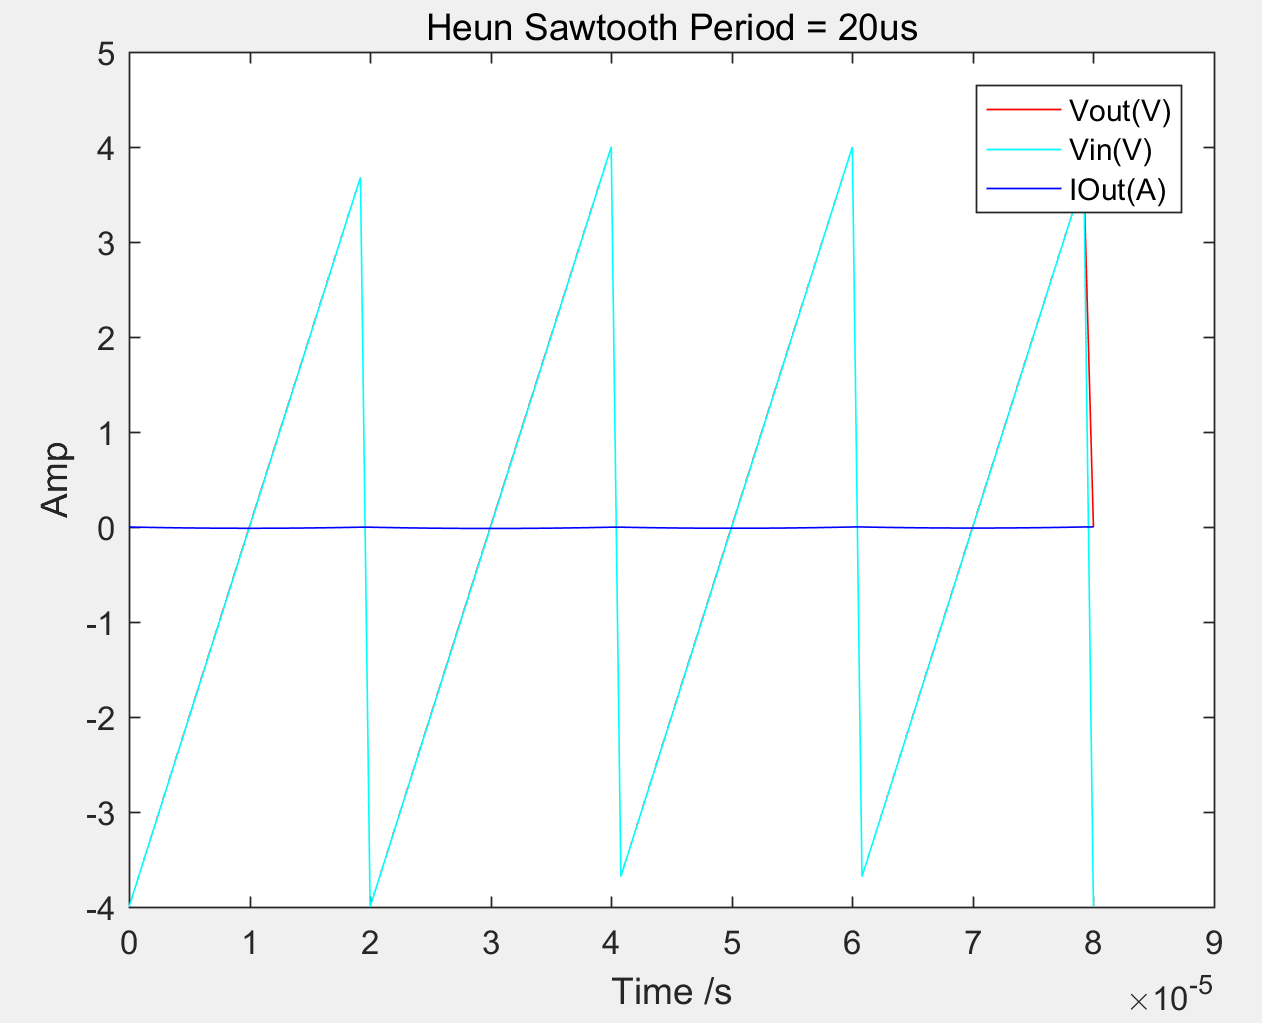
\includegraphics[width=\textwidth]{ex1/heun_sawtooth_20.PNG}
            \caption{Heun sawtooth T=20}
      \end{subfigure}
      ~
      \begin{subfigure}[b]{0.4\textwidth}
            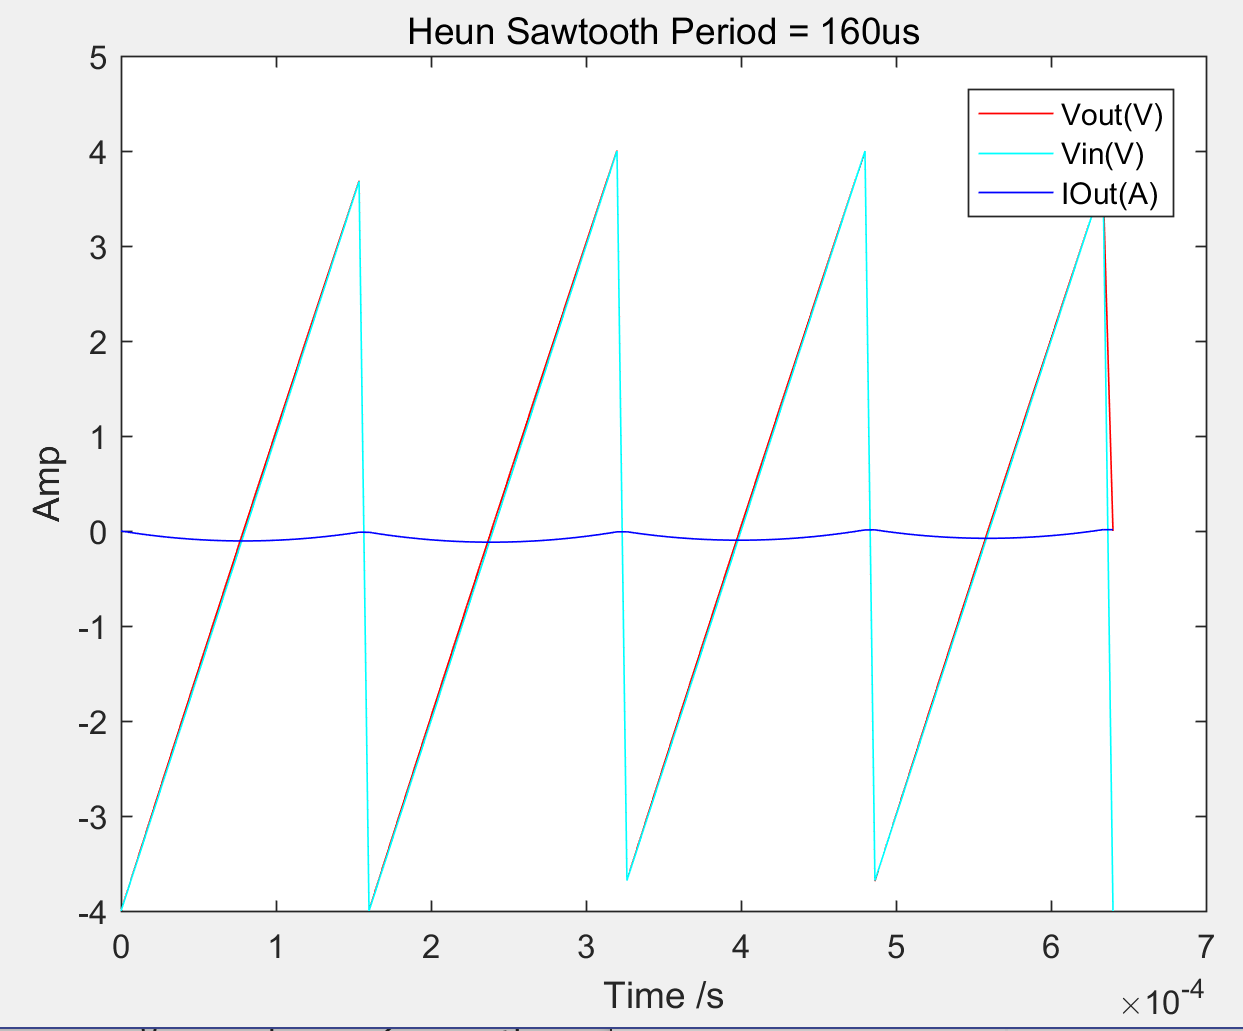
\includegraphics[width=\textwidth]{ex1/heun_sawtooth_160.PNG}
            \caption{Heun sawtooth T=160}
      \end{subfigure}
       ~
      \begin{subfigure}[b]{0.4\textwidth}
            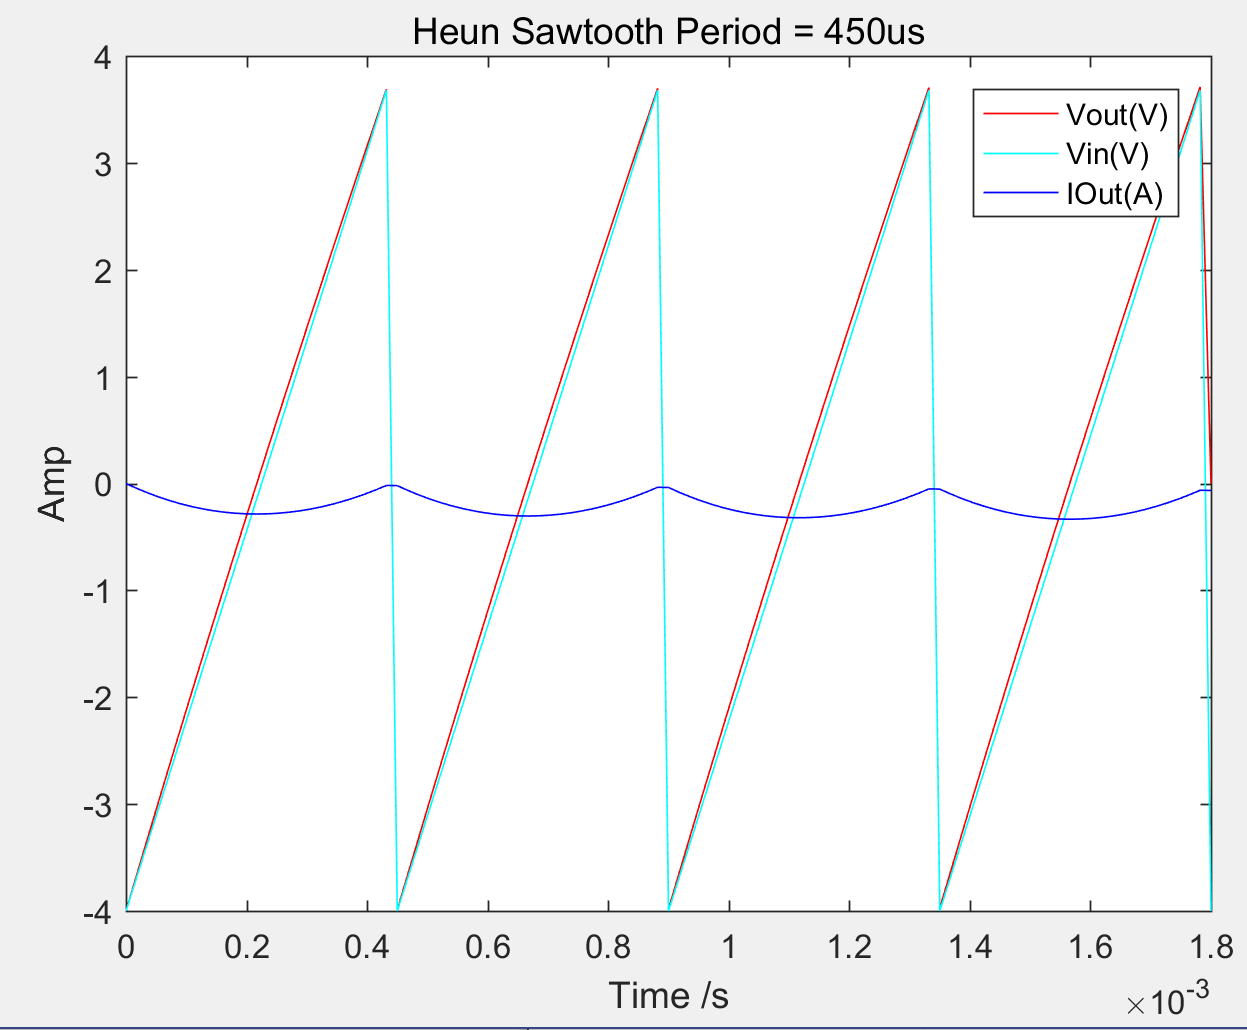
\includegraphics[width=\textwidth]{ex1/heun_sawtooth_450PNG.PNG}
            \caption{Heun sawtooth T=450}
      \end{subfigure}
       ~
      \begin{subfigure}[b]{0.4\textwidth}
            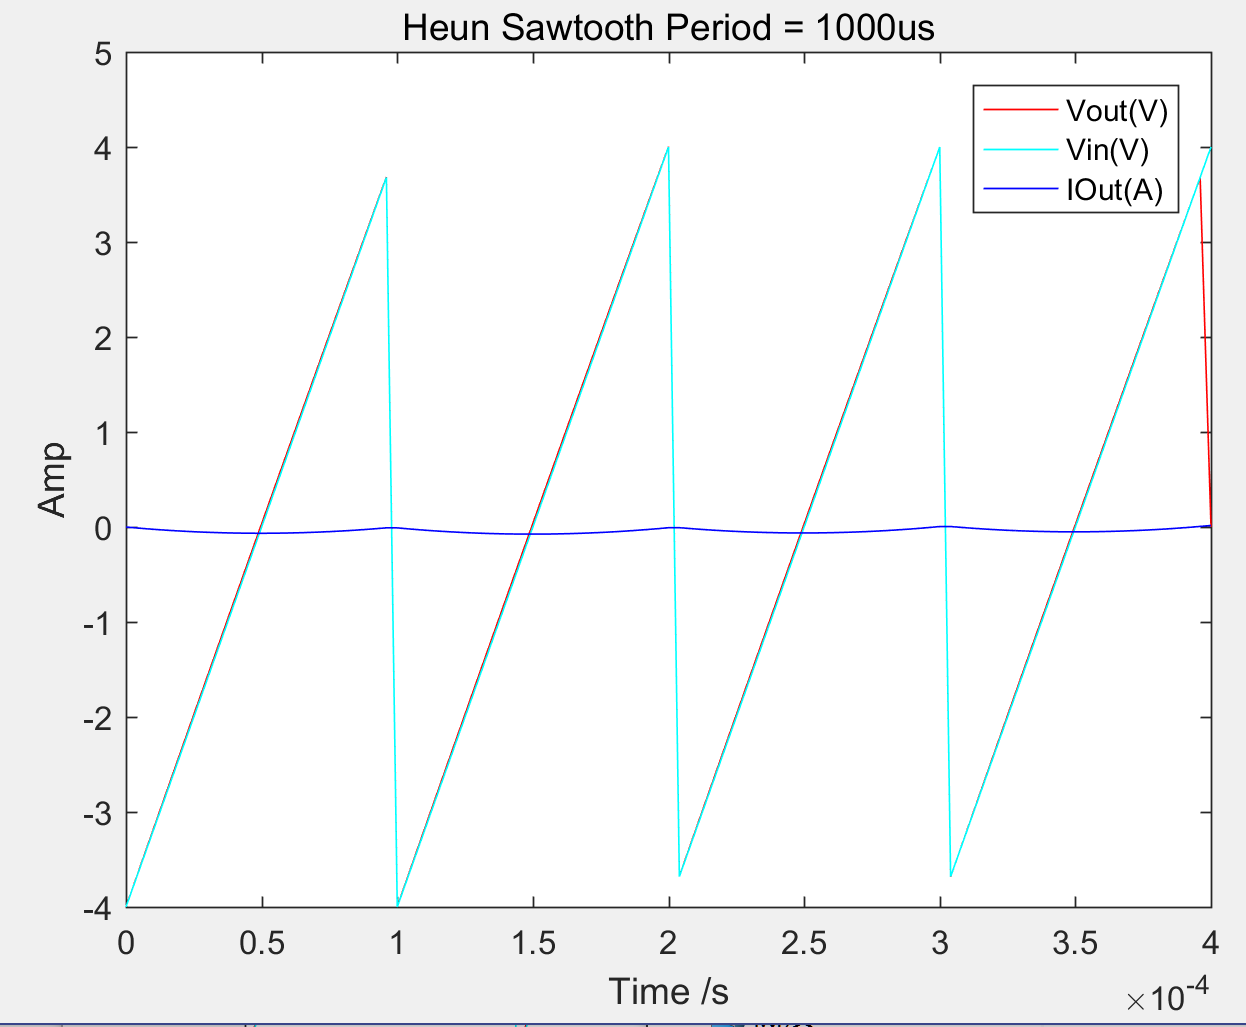
\includegraphics[width=\textwidth]{ex1/heun_sawtooth_1000.PNG}
            \caption{Heun sawtooth T=1000}
      \end{subfigure}
      \caption{Heun's method}
\end{figure}

\newpage
And the following plots are for Midpoint and Ralston methods:
\begin{figure}[h]
      \centering
      \begin{subfigure}[b]{0.4\textwidth}
            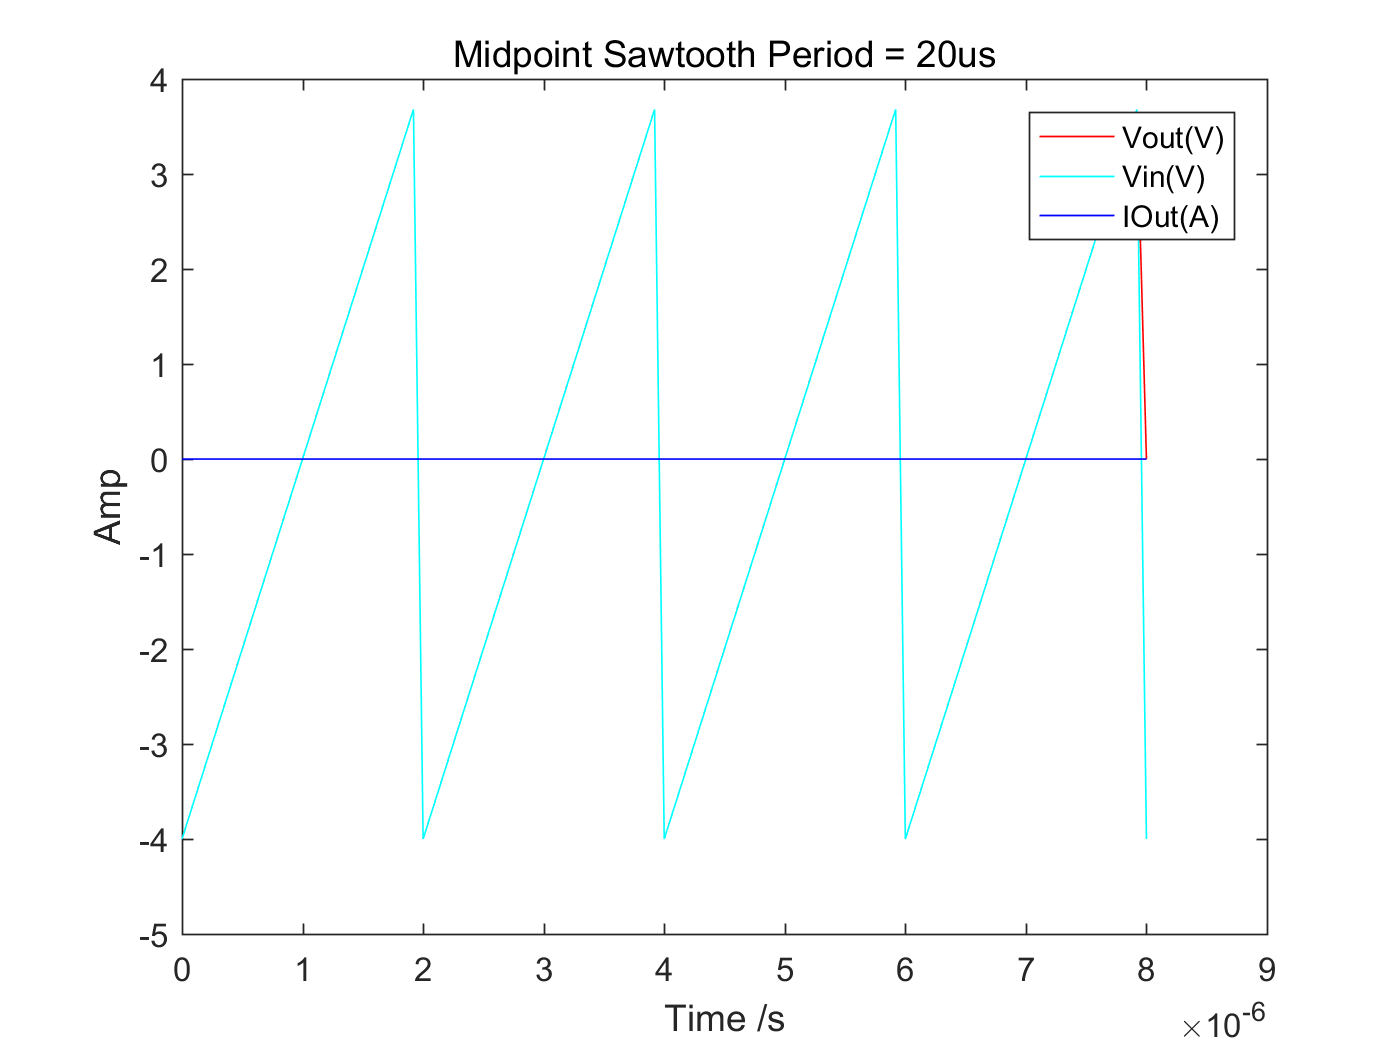
\includegraphics[width=\textwidth]{ex1/new_mid_sawtooth_20.PNG}
            \caption{Midpoint sawtooth T=20}
      \end{subfigure}
      ~
      \begin{subfigure}[b]{0.4\textwidth}
            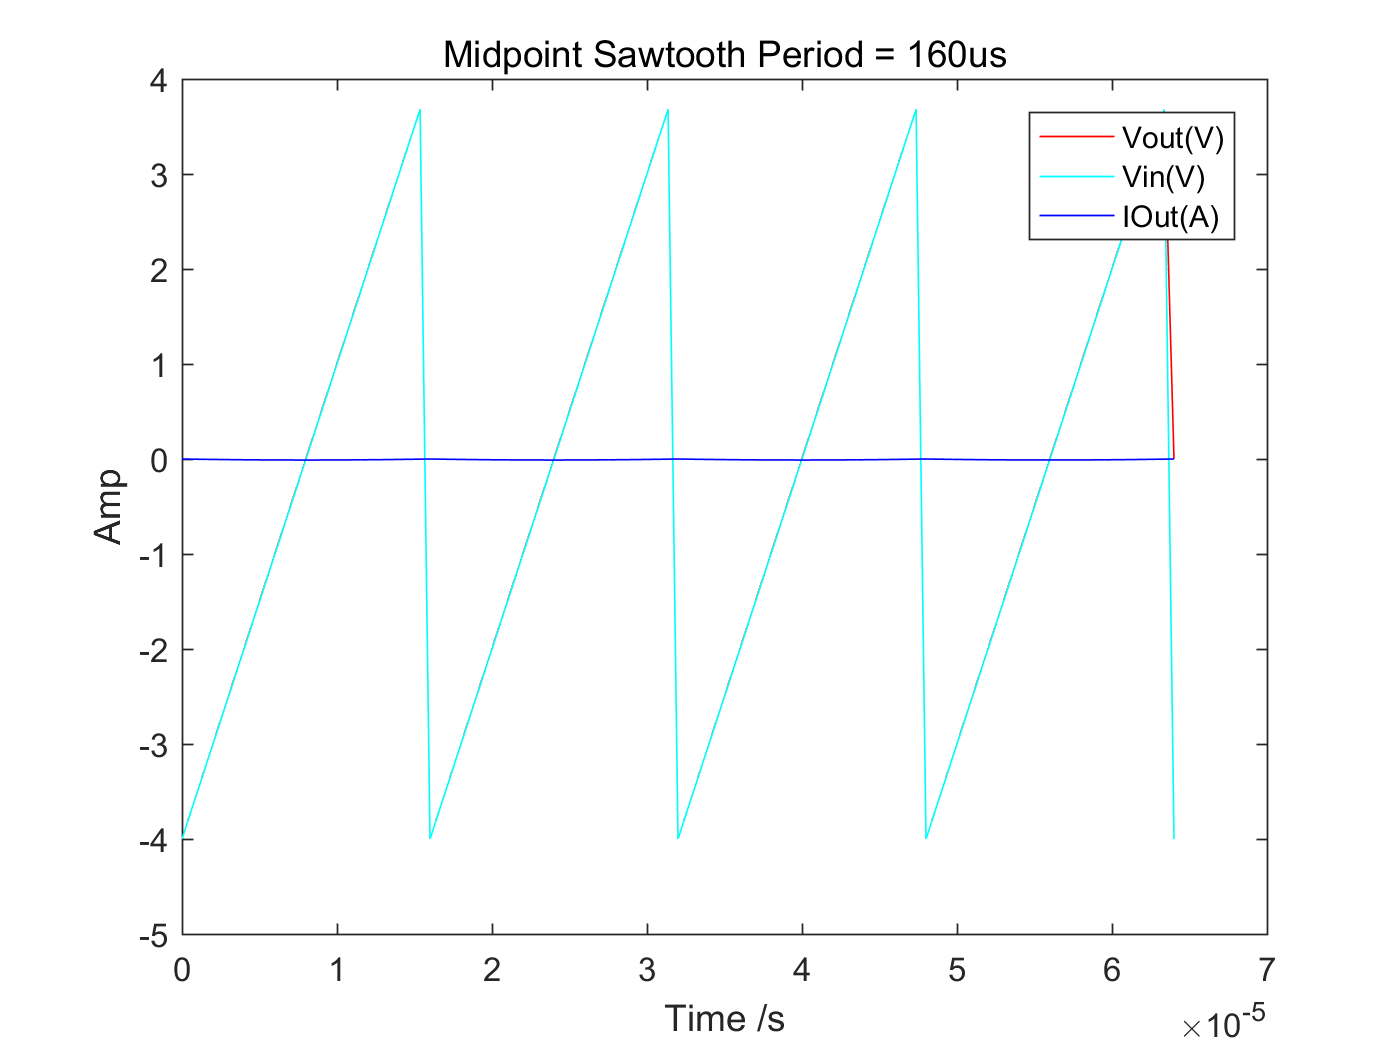
\includegraphics[width=\textwidth]{ex1/new_mid_sawtooth_160.PNG}
            \caption{Midpoint sawtooth T=160}
      \end{subfigure}
       ~
      \begin{subfigure}[b]{0.4\textwidth}
            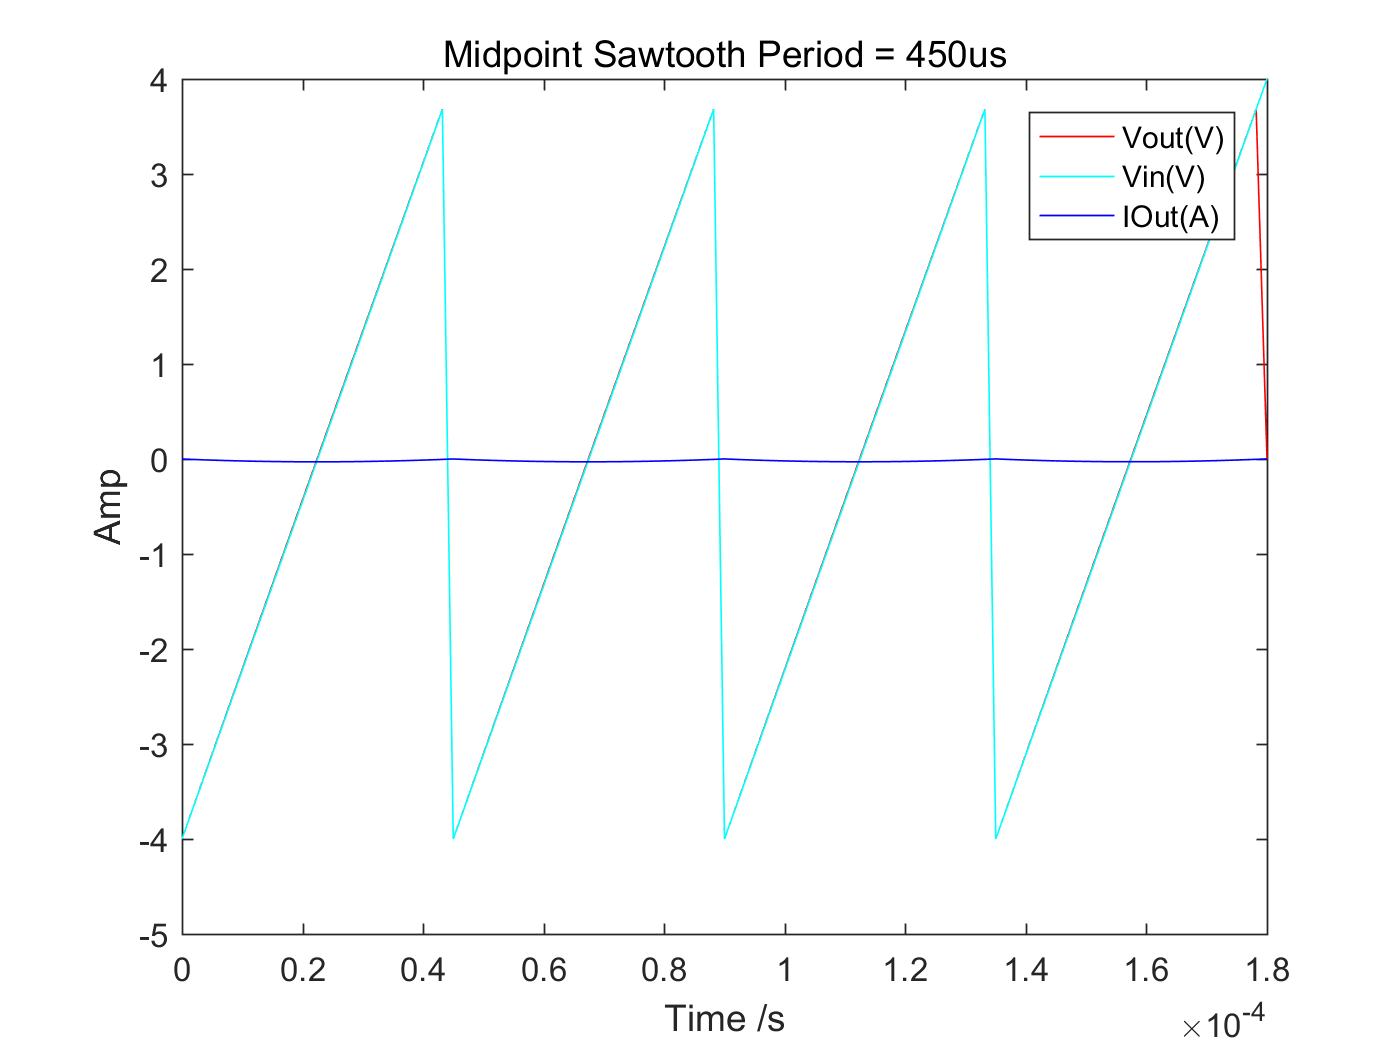
\includegraphics[width=\textwidth]{ex1/new_mid_sawtooth_450.PNG}
            \caption{Midpoint sawtooth T=450}
      \end{subfigure}
       ~
      \begin{subfigure}[b]{0.4\textwidth}
            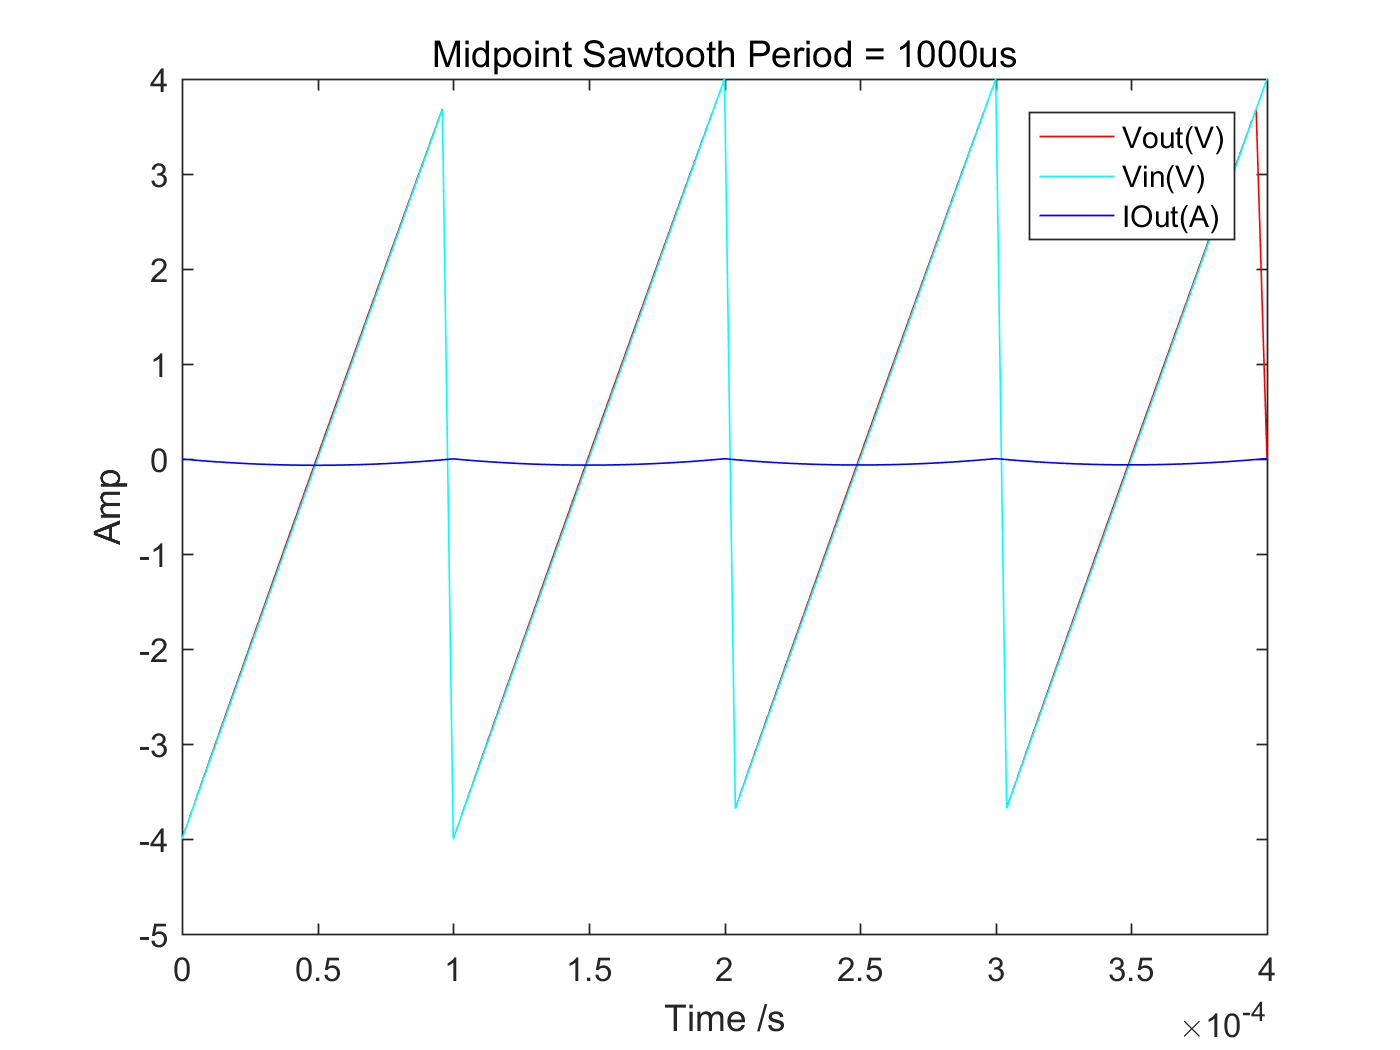
\includegraphics[width=\textwidth]{ex1/new_midpoint_saw_1000.png}
            \caption{Midpoint sawtooth T=1000}
      \end{subfigure}
      \caption{Midpoint method}
\end{figure}
\newpage
\begin{figure}[h]
      \centering
      \begin{subfigure}[b]{0.4\textwidth}
            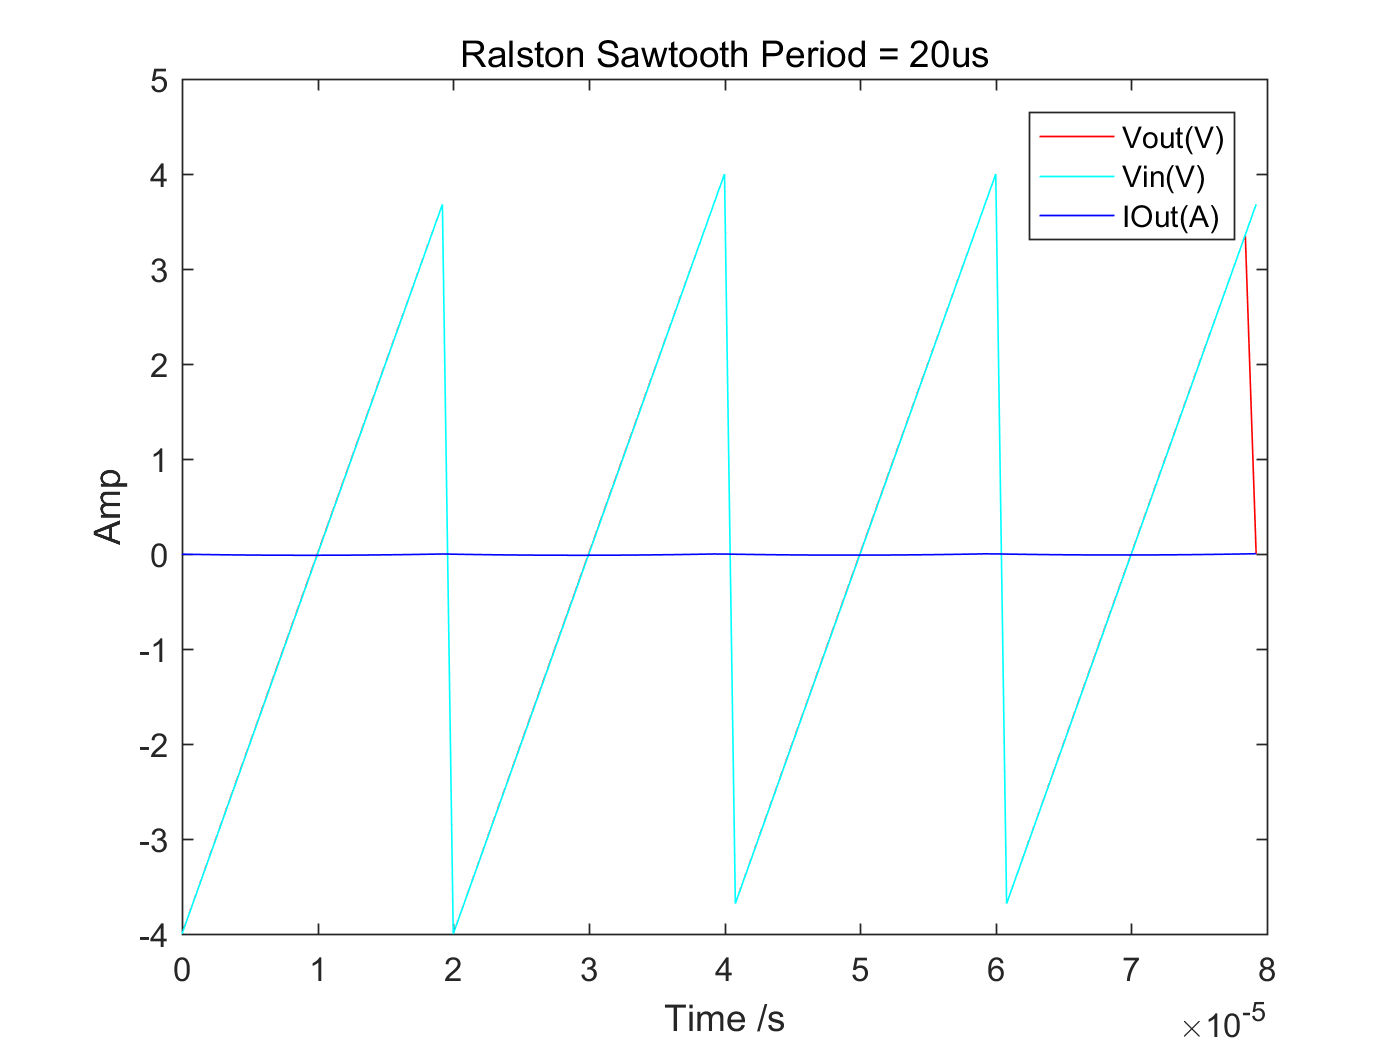
\includegraphics[width=\textwidth]{ex1/ralston_sawtooth_20.png}
            \caption{Ralston sawtooth T=20}
      \end{subfigure}
      ~
      \begin{subfigure}[b]{0.4\textwidth}
            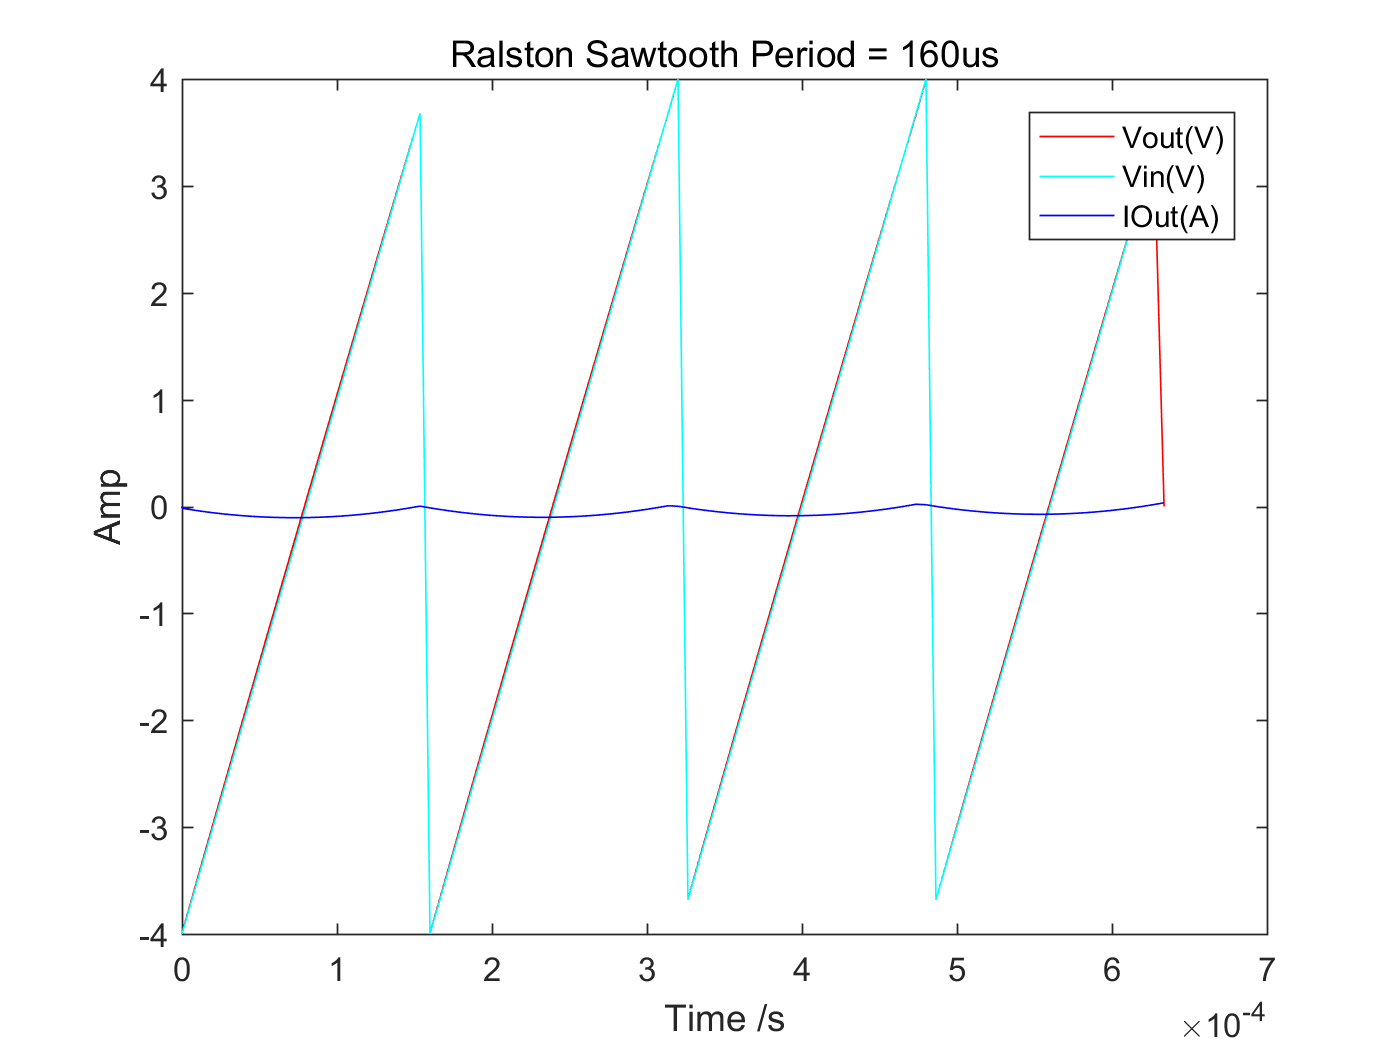
\includegraphics[width=\textwidth]{ex1/ralston_sawtooth_160.png}
            \caption{Ralston sawtooth T=160}
      \end{subfigure}
       ~
      \begin{subfigure}[b]{0.4\textwidth}
            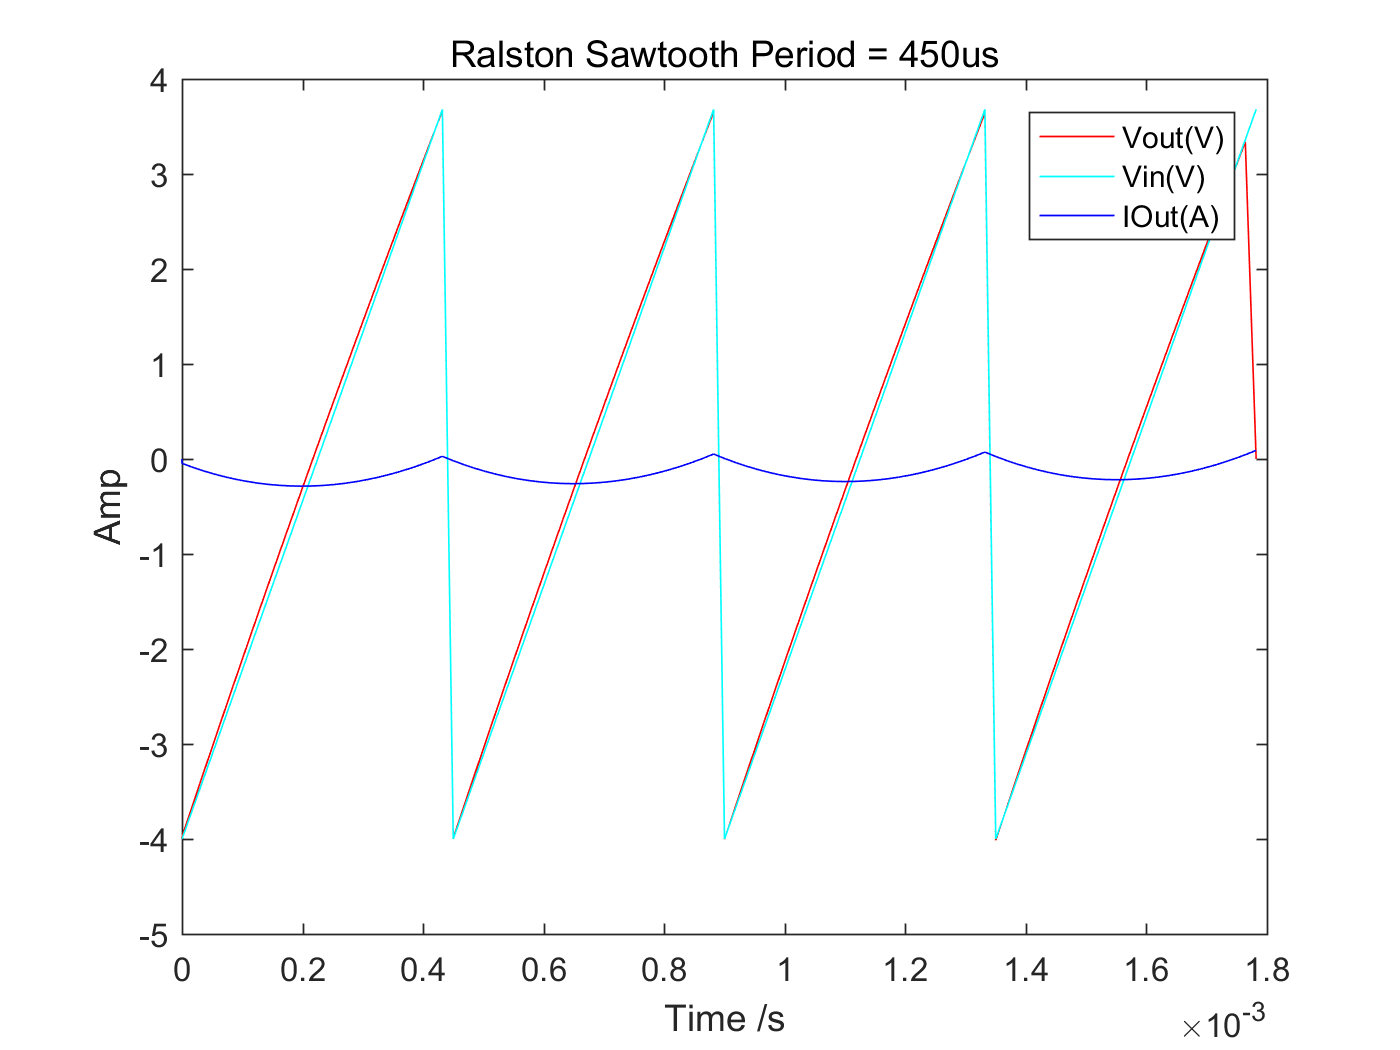
\includegraphics[width=\textwidth]{ex1/ralston_sawtooth_450.png}
            \caption{Ralston sawtooth T=450}
      \end{subfigure}
       ~
      \begin{subfigure}[b]{0.4\textwidth}
            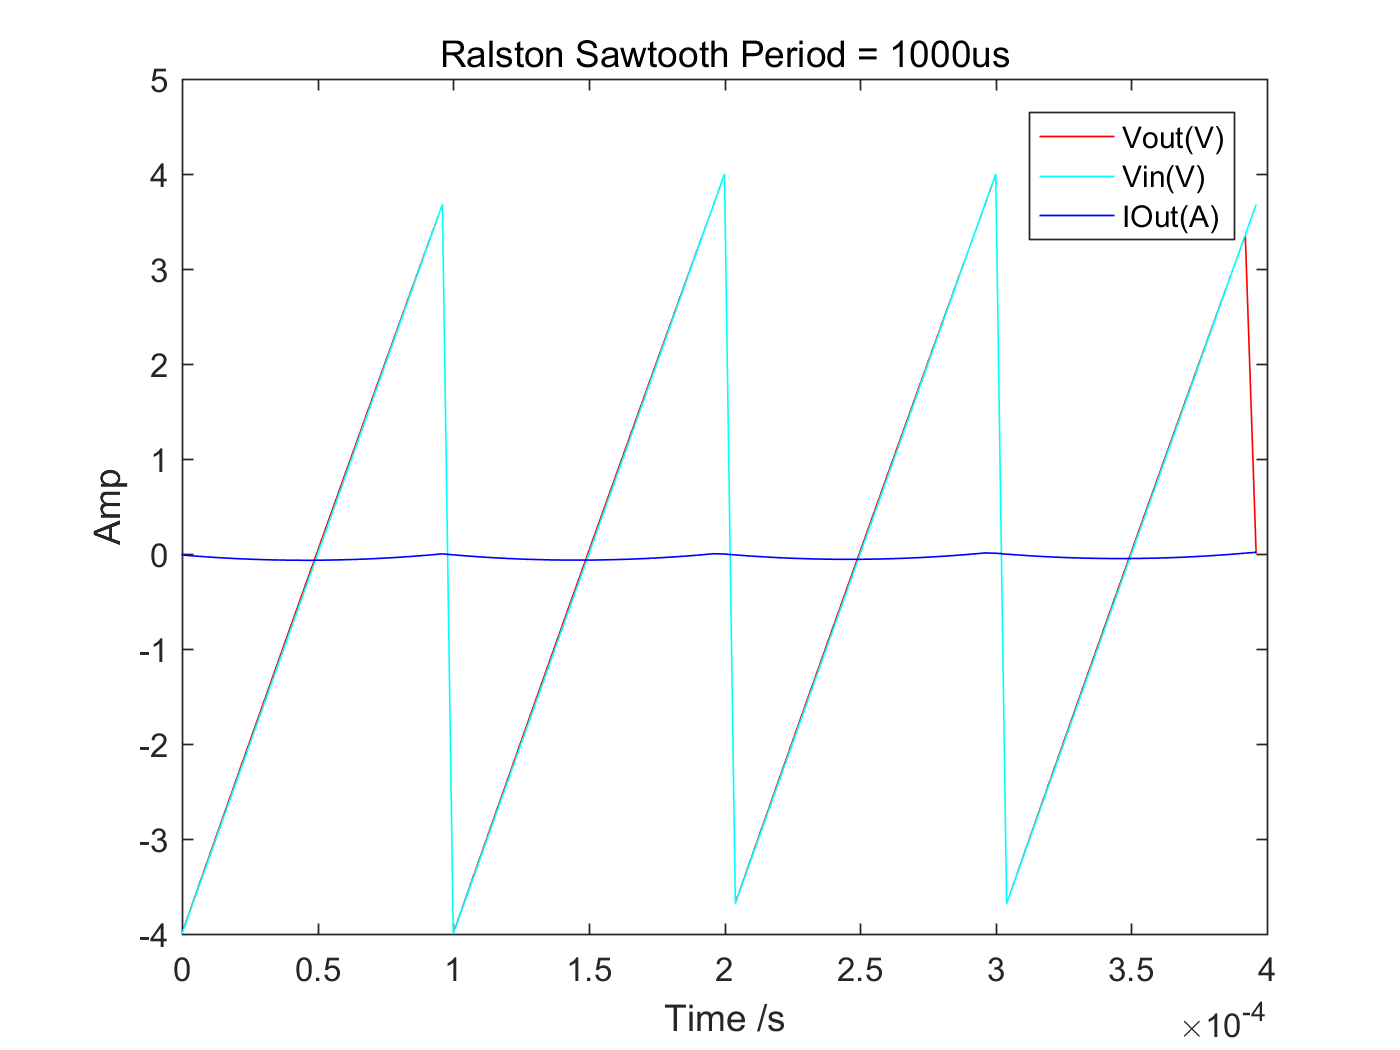
\includegraphics[width=\textwidth]{ex1/ralston_sawtooth_1000.png}
            \caption{Ralston sawtooth T=1000}
      \end{subfigure}
      \caption{Ralston method}
\end{figure}
\begin{equation}\label{inductor2}
V_{L} = V_{in}e^{-tR/L}
\end{equation} 
When we input a sawtooth wave into the RL series circuit, the inductor becomes like an open circuit at first, so it takes most of the input voltage and when the sawtooth changes from highest point to lowest point, from equation (6), we can see that the voltage across the inductor is dependent on the input voltage with exponential decrement. We can assume the voltage in the sawtooth wave is rapidly changing, so the voltage across the inductor is also change rapidly.   \par

\newpage

\subsubsection{Square input}
In this part, we input a Square wave into the circuit(Heun's Method). In this part, there is also no Vout phase shift or distortion when period is equal to 20us:
\begin{figure}[h]
      \centering
      \begin{subfigure}[b]{0.4\textwidth}
            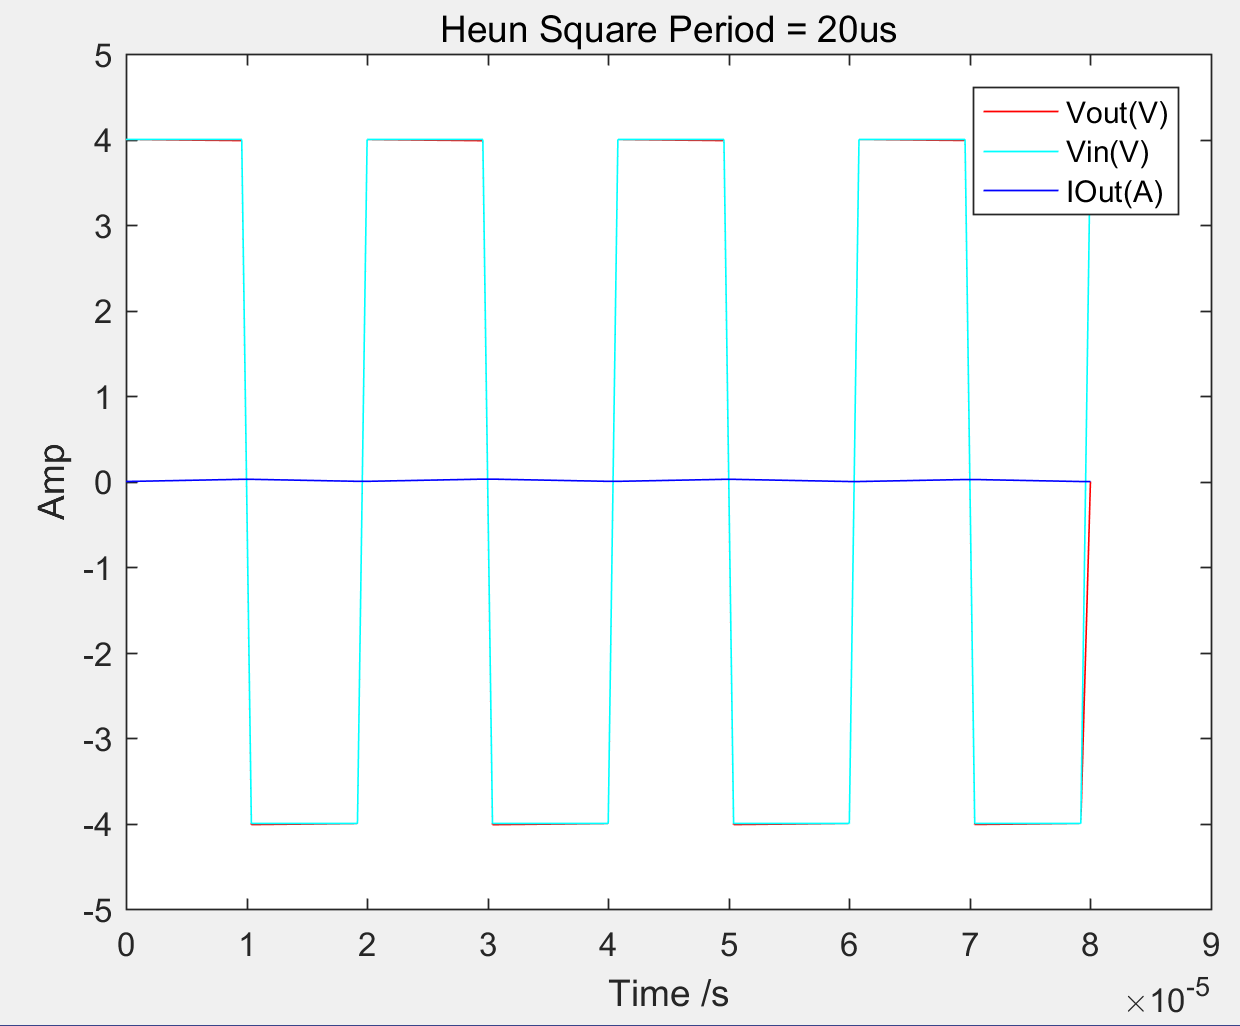
\includegraphics[width=\textwidth]{ex1/heun_square_20.PNG}
            \caption{Heun square T=20}
      \end{subfigure}
      ~
      \begin{subfigure}[b]{0.4\textwidth}
            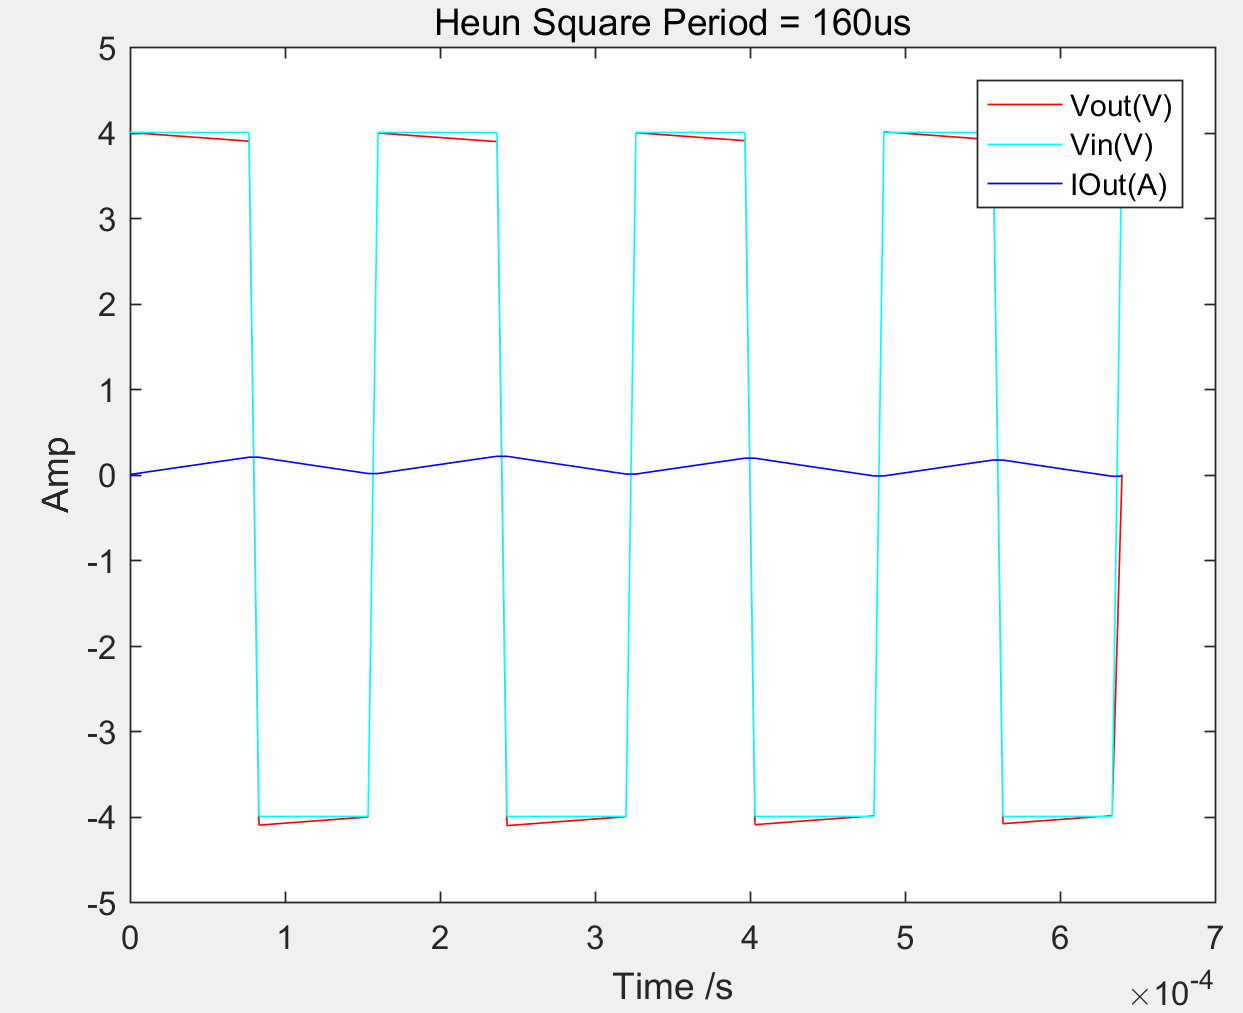
\includegraphics[width=\textwidth]{ex1/heun_square_160.PNG}
            \caption{Heun square T=160}
      \end{subfigure}
       ~
      \begin{subfigure}[b]{0.4\textwidth}
            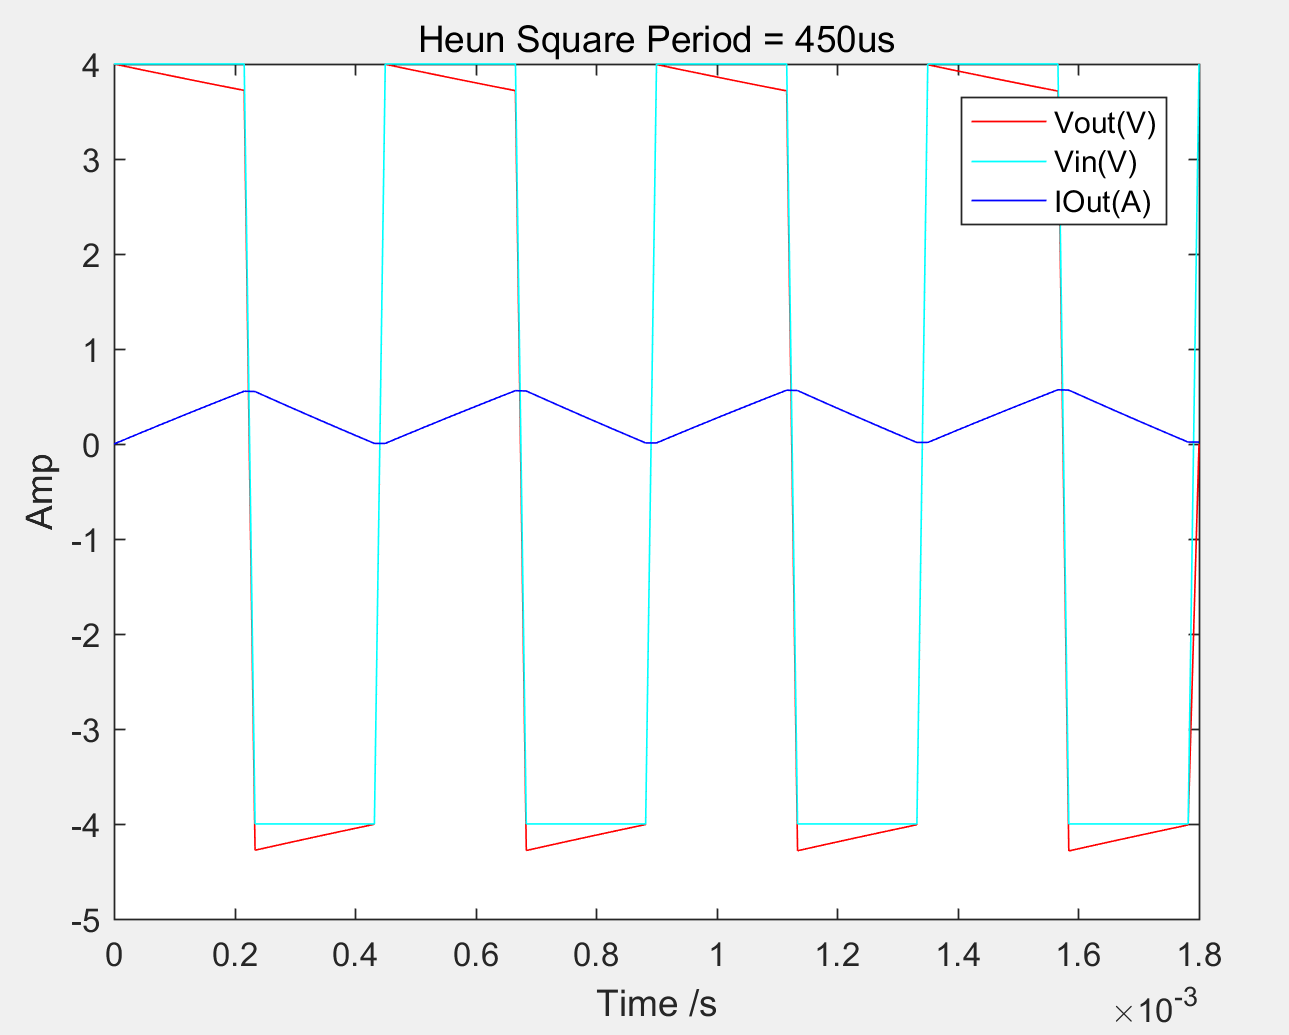
\includegraphics[width=\textwidth]{ex1/heun_square_450.PNG}
            \caption{Heun square T=450}
      \end{subfigure}
       ~
      \begin{subfigure}[b]{0.4\textwidth}
            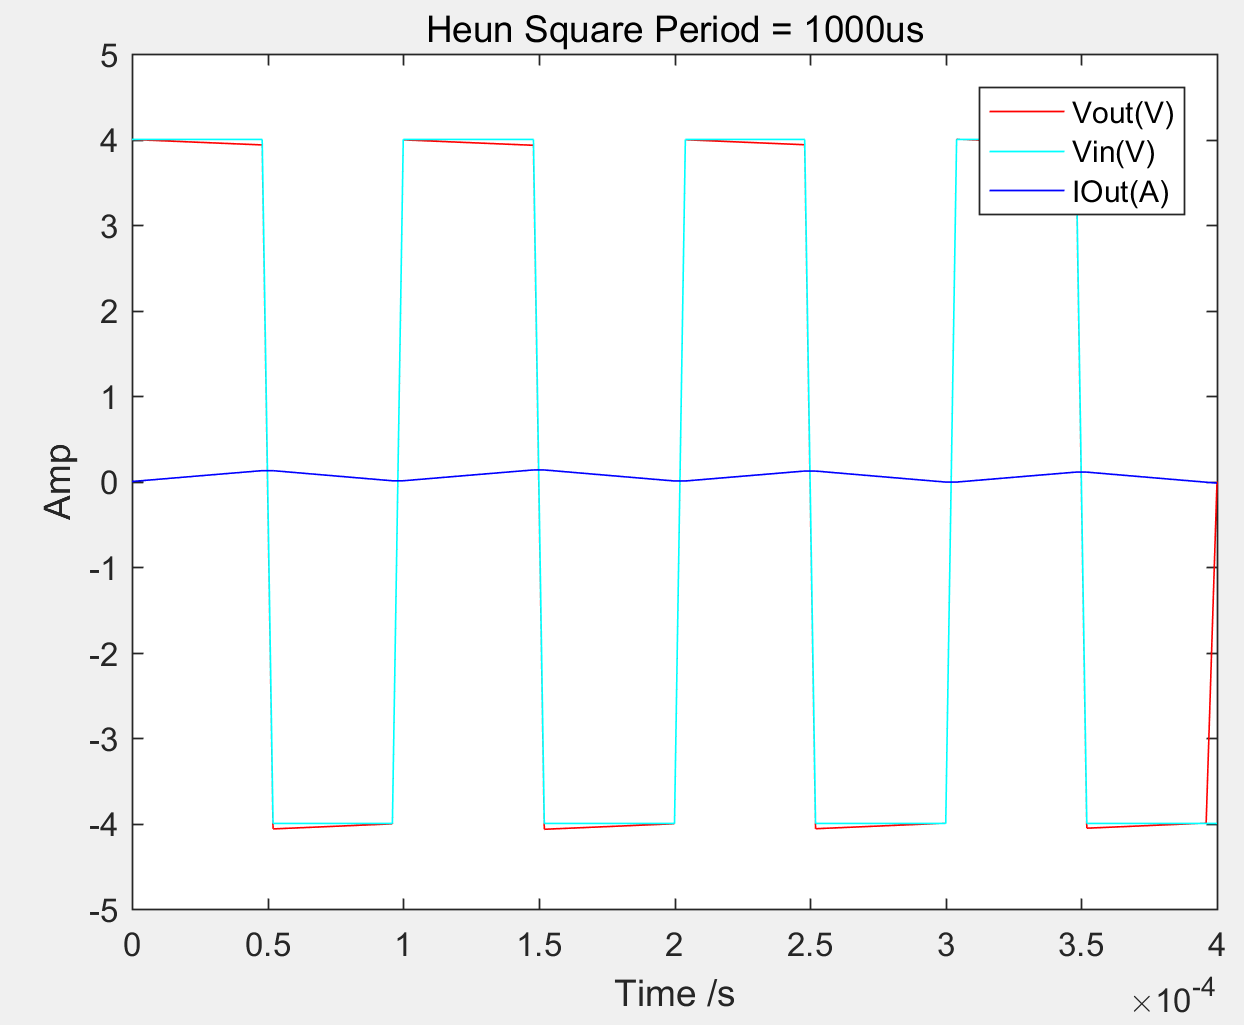
\includegraphics[width=\textwidth]{ex1/heun_square_1000.PNG}
            \caption{Heun square T=1000}
      \end{subfigure}
      \caption{Heun's method}
\end{figure}

\newpage
And the following plots are for Midpoint and Ralston methods:
\begin{figure}[h]
      \centering
      \begin{subfigure}[b]{0.4\textwidth}
            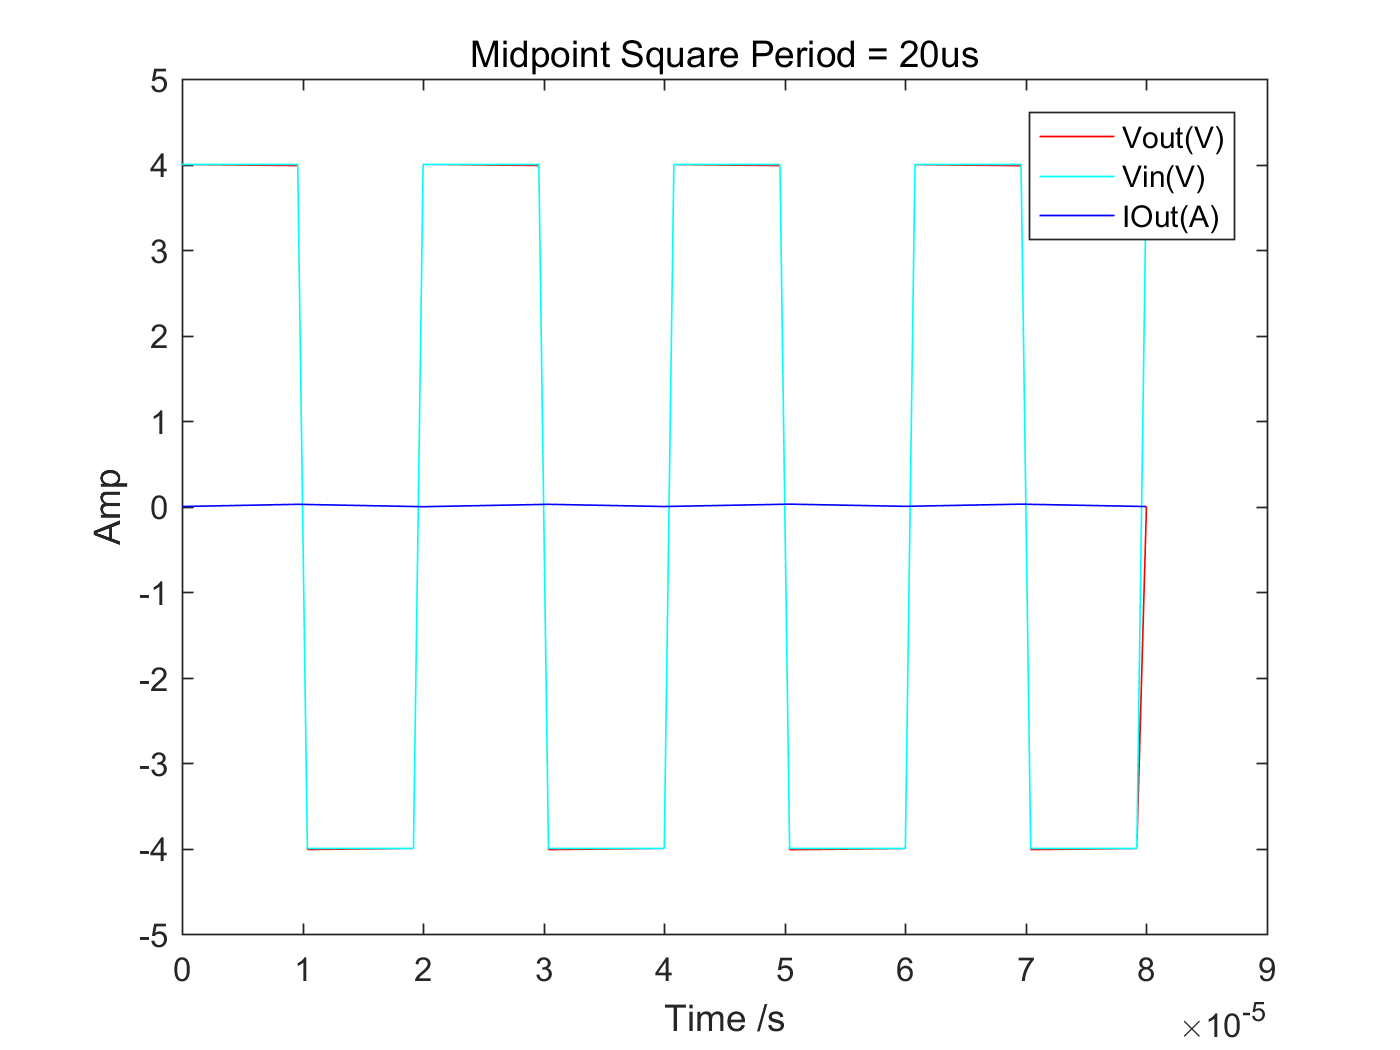
\includegraphics[width=\textwidth]{ex1/midpoint_square_20.png}
            \caption{Midpoint square T=20}
      \end{subfigure}
      ~
      \begin{subfigure}[b]{0.4\textwidth}
            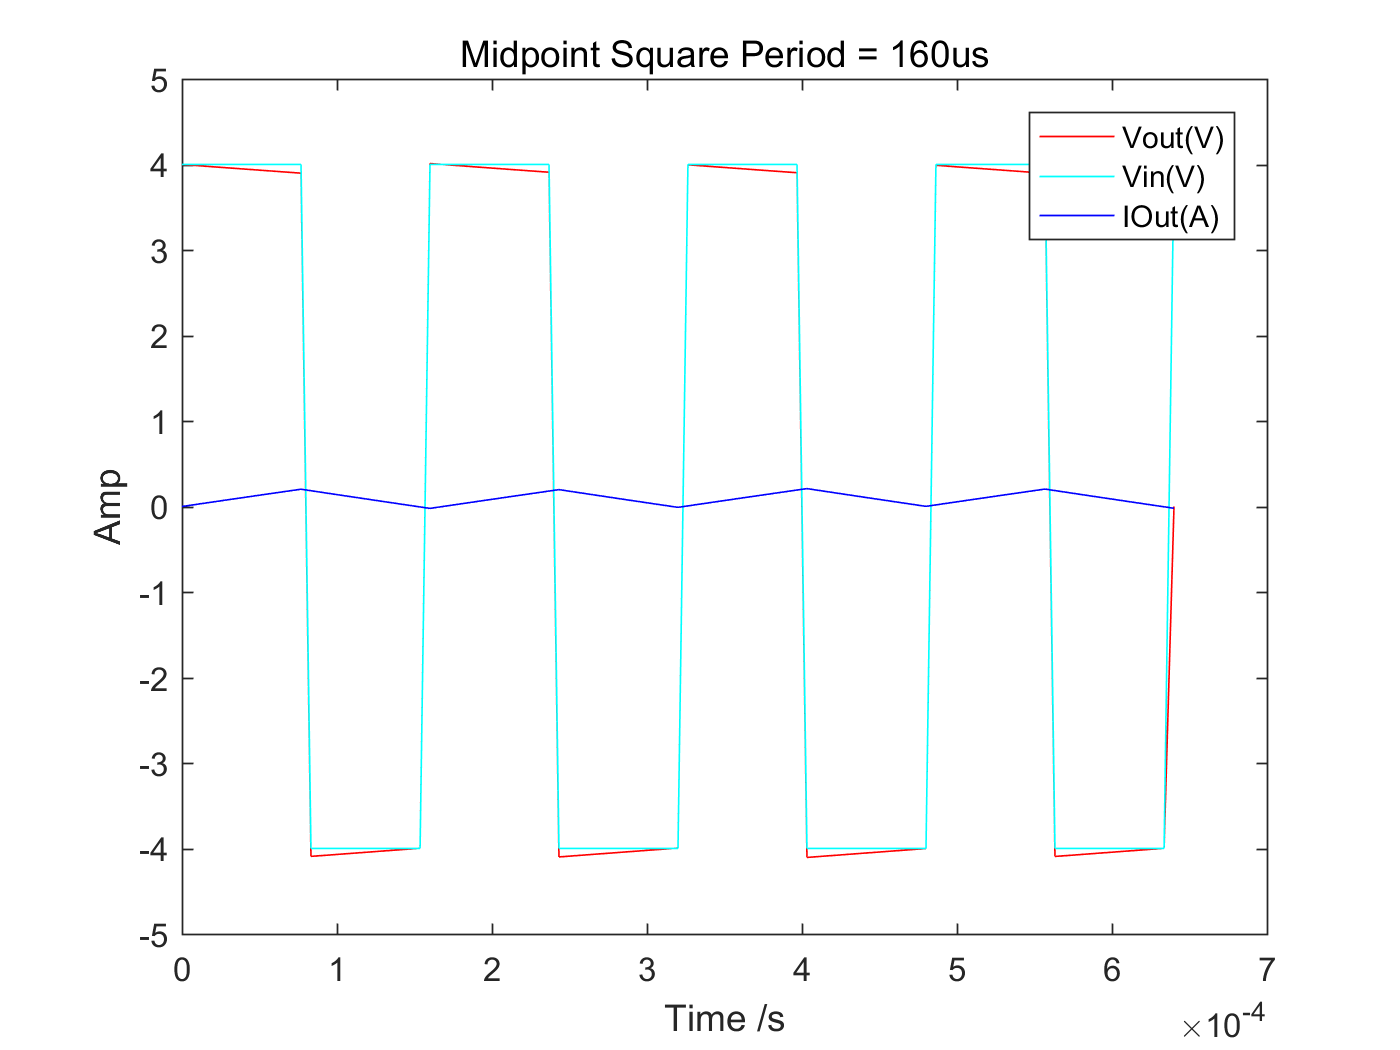
\includegraphics[width=\textwidth]{ex1/midpoint_square_160.png}
            \caption{Midpoint square T=160}
      \end{subfigure}
       ~
      \begin{subfigure}[b]{0.4\textwidth}
            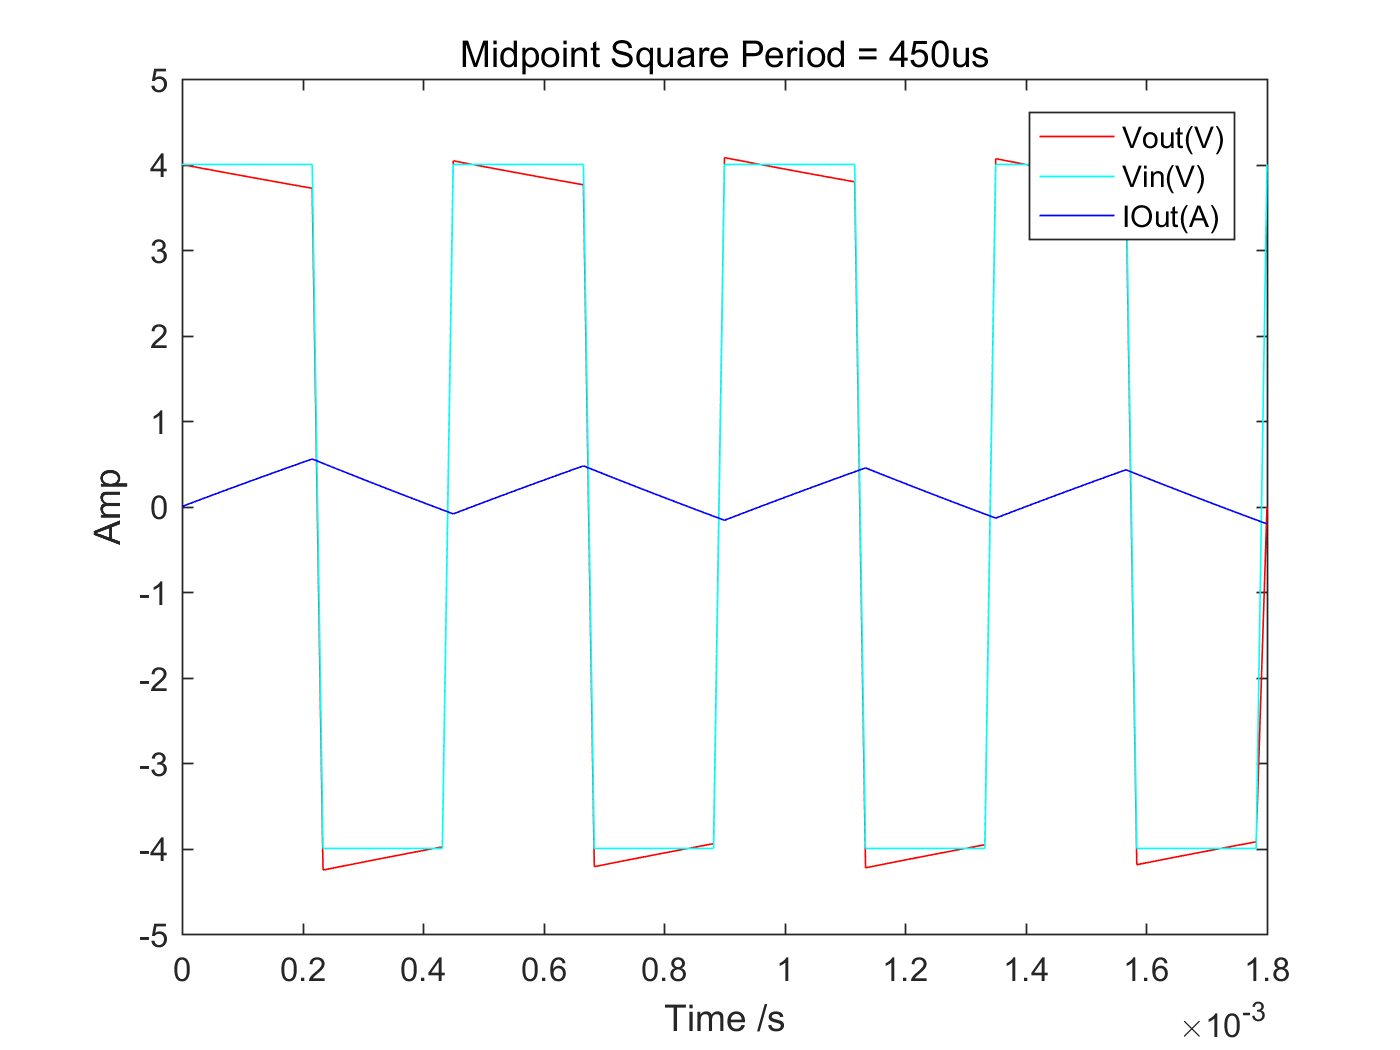
\includegraphics[width=\textwidth]{ex1/midpoint_square_450.png}
            \caption{Midpoint square T=450}
      \end{subfigure}
       ~
      \begin{subfigure}[b]{0.4\textwidth}
            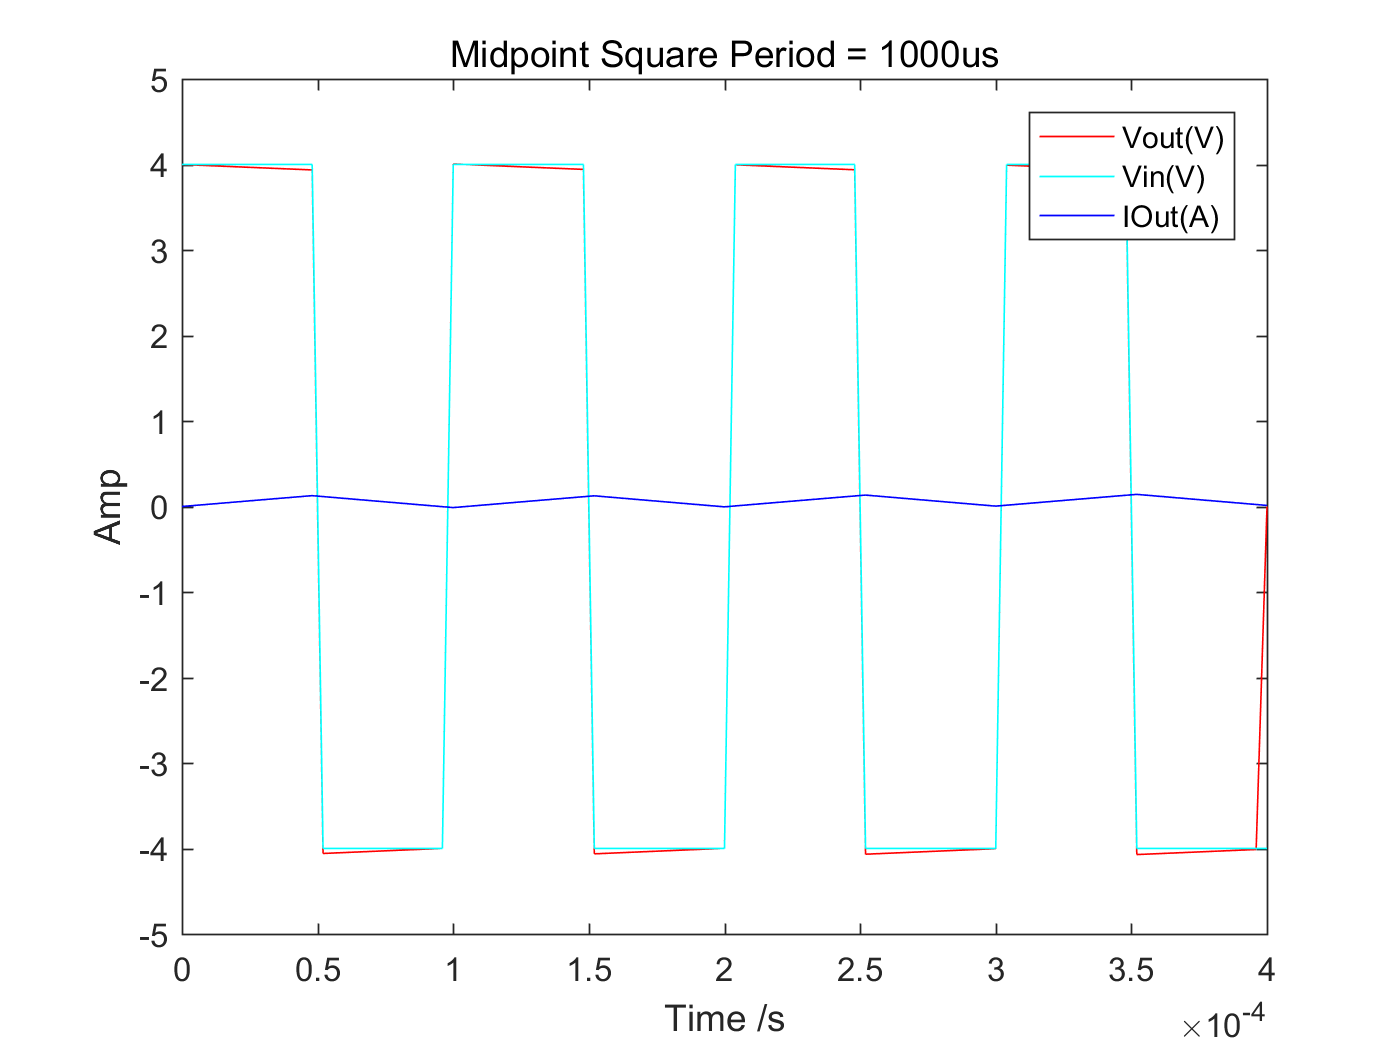
\includegraphics[width=\textwidth]{ex1/midpoint_square_1000.png}
            \caption{Midpoint square T=1000}
      \end{subfigure}
      \caption{Midpoint method}
\end{figure}
\newpage
\begin{figure}[h]
      \centering
      \begin{subfigure}[b]{0.4\textwidth}
            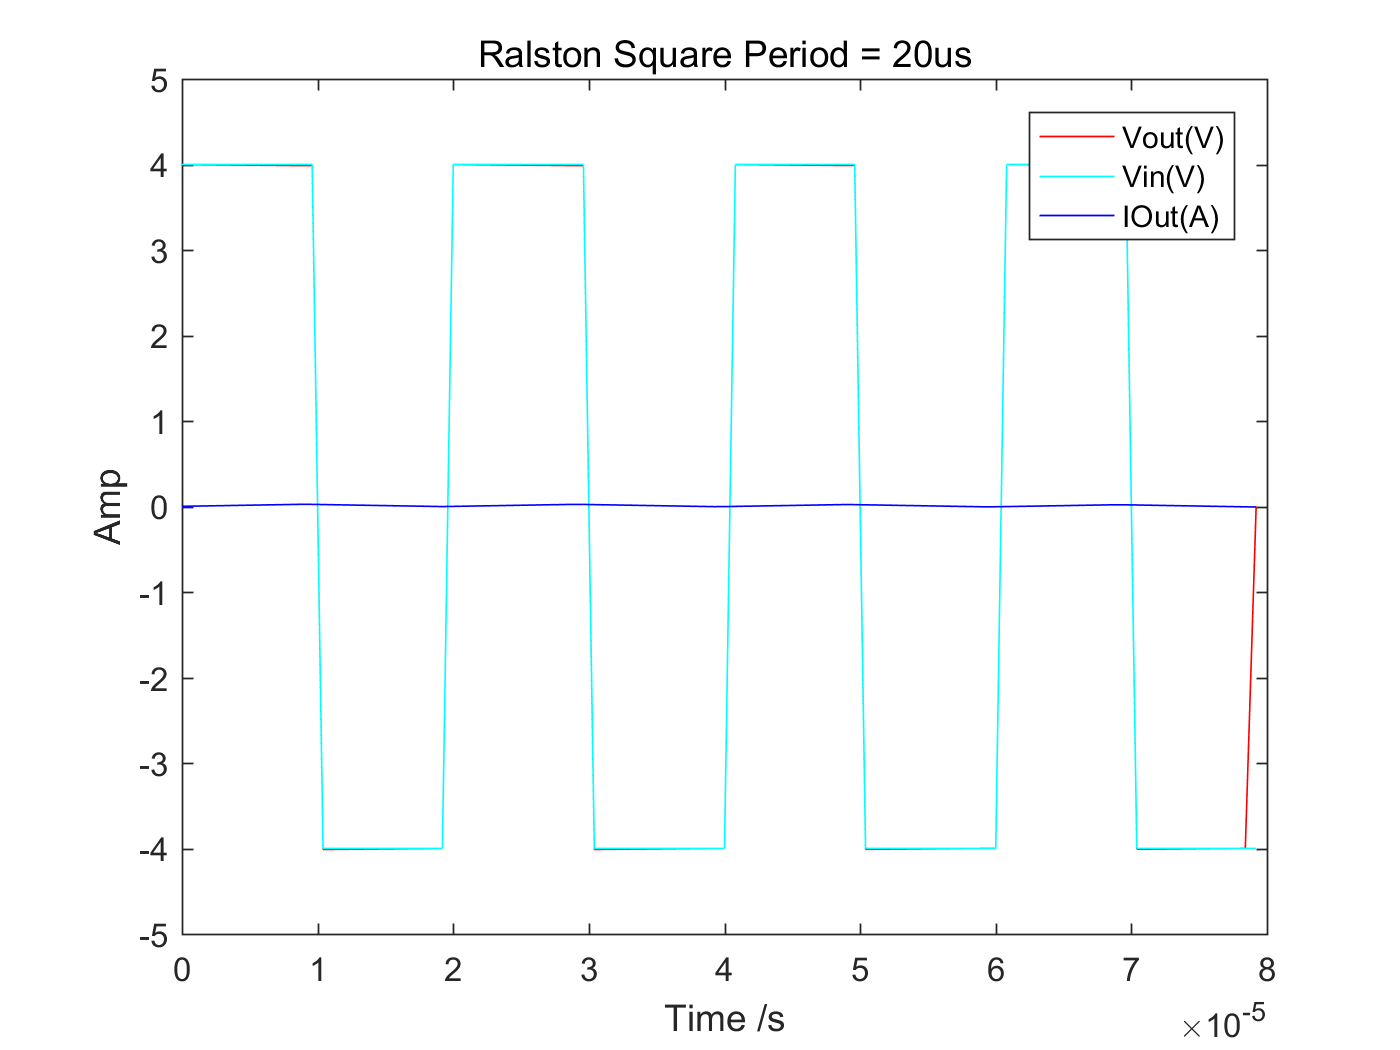
\includegraphics[width=\textwidth]{ex1/new_ralston_square_20.png}
            \caption{Ralston square T=20}
      \end{subfigure}
      ~
      \begin{subfigure}[b]{0.4\textwidth}
            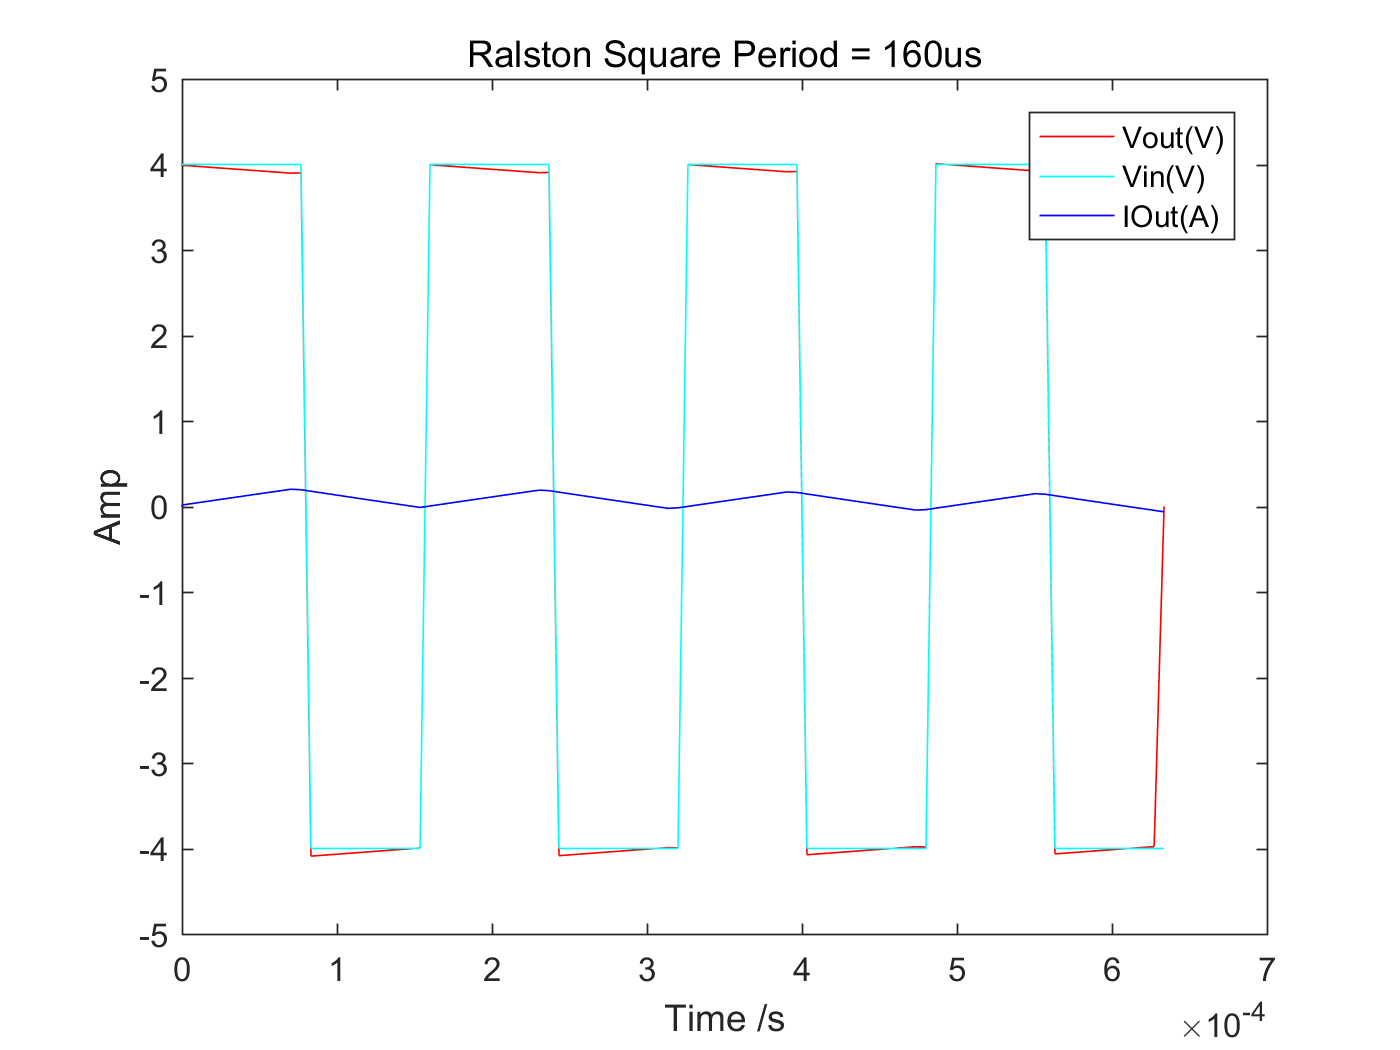
\includegraphics[width=\textwidth]{ex1/new_ralston_square_160.png}
            \caption{Ralston square T=160}
      \end{subfigure}
       ~
      \begin{subfigure}[b]{0.4\textwidth}
            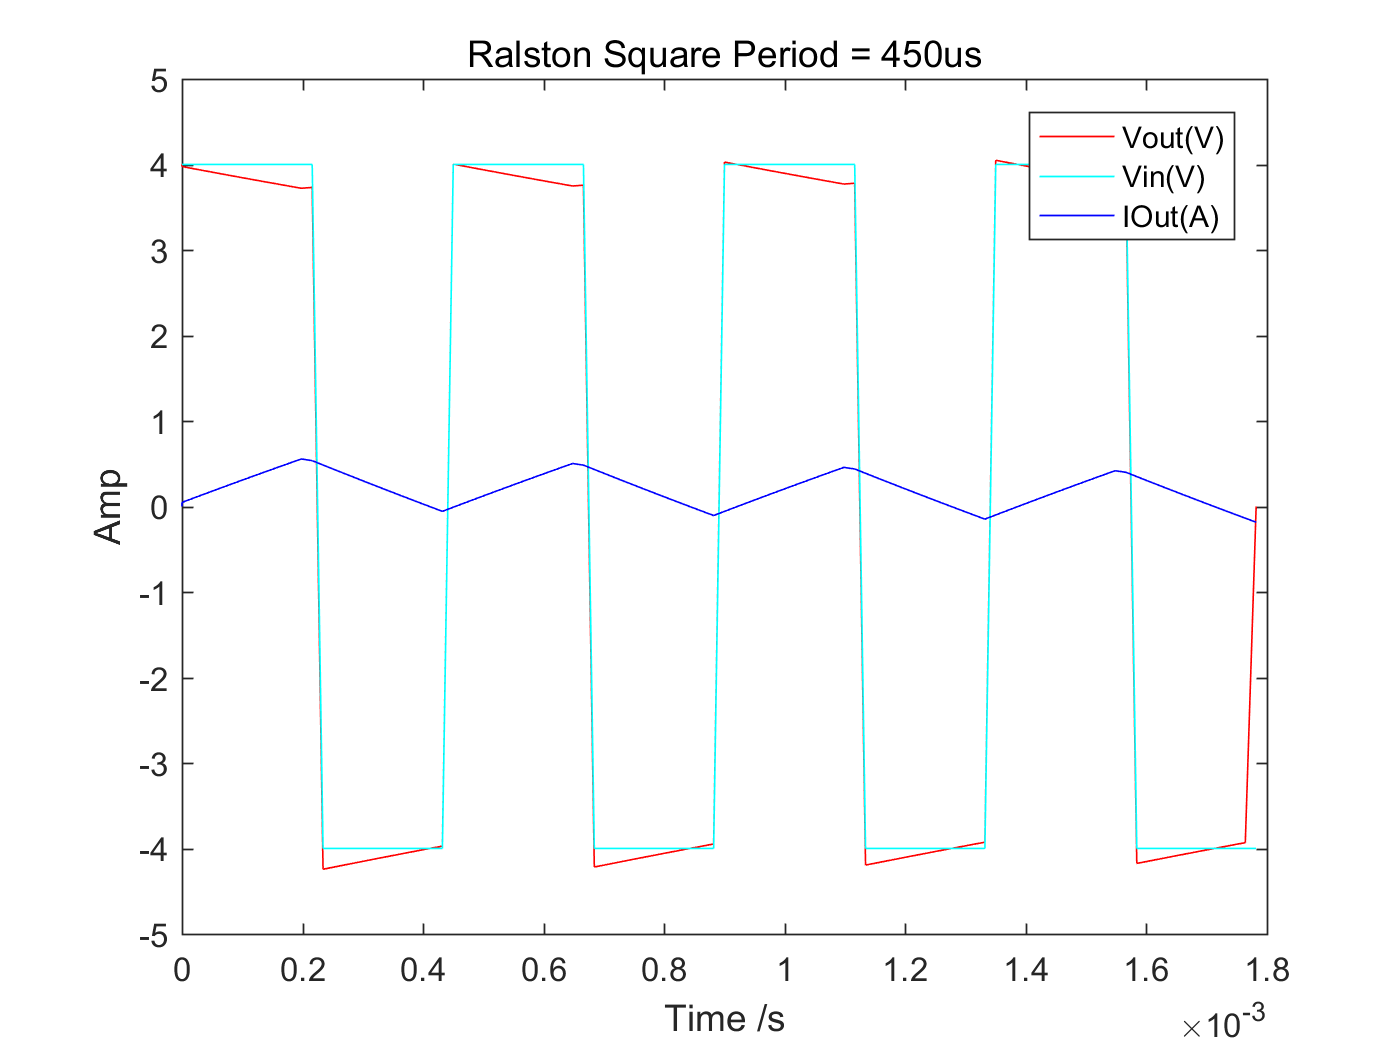
\includegraphics[width=\textwidth]{ex1/new_ralston_square_450.png}
            \caption{Ralston square T=450}
      \end{subfigure}
       ~
      \begin{subfigure}[b]{0.4\textwidth}
            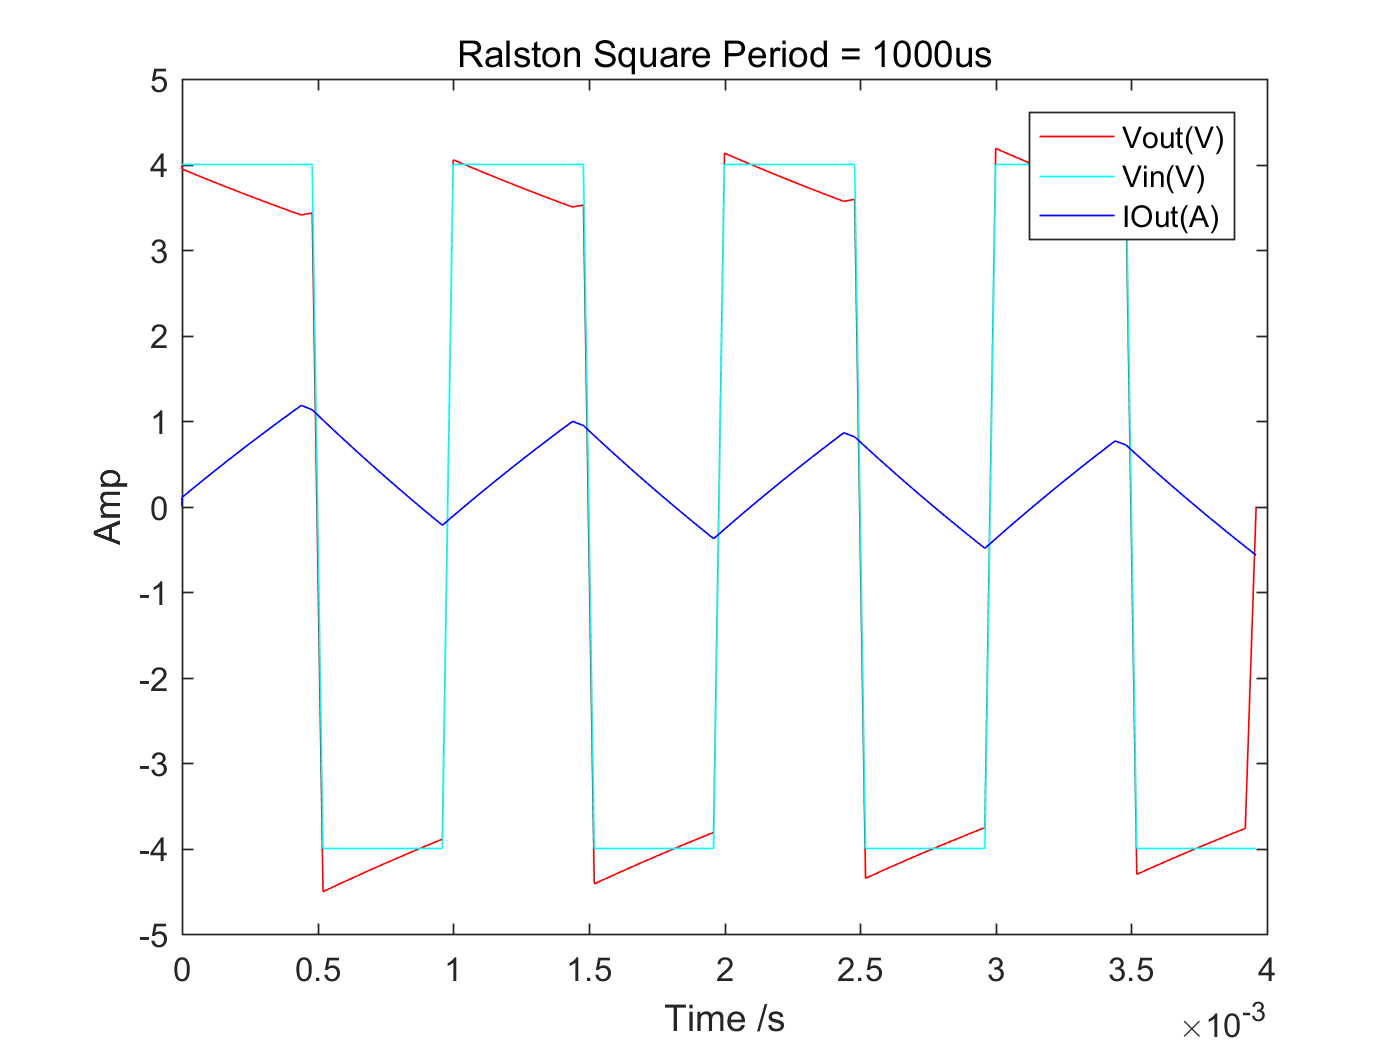
\includegraphics[width=\textwidth]{ex1/new_ralston_square_1000.png}
            \caption{Ralston square T=1000}
      \end{subfigure}
      \caption{Ralston method}
\end{figure}
From the plots above, we can see that when the frequency is greater than 450us, the output voltage becomes more inaccurate and distorted.\par
\vspace{5mm}
At first, the inductor acts as an open circuit. When we input a square wave into the circuit, the voltage across the inductor starts to drop, and the voltage across the resistor increases instead. So from the screen shot above, we can see that when the time period of the wave increases, the drop appears to be more abrupt. Hence we get the result above.\cite{waveformoutput}
\newpage
\subsubsection{MATLAB codes}
\lstinputlisting[caption = heun.m]{ex1/heun.m}\par
\lstinputlisting[caption = heun script.m]{ex1/heun_script_q3.m}
\lstinputlisting[caption = midpoint.m]{ex1/midpoint.m}\par
\lstinputlisting[caption = midpoint script.m]{ex1/midpoint_script_q3.m}
\lstinputlisting[caption = ralston.m]{ex1/ralston.m}\par
\lstinputlisting[caption = ralston script.m]{ex1/ralston_script_q3.m}

\newpage
\subsection{Error Analysis}\FloatBarrier
Given as input:
\[
      V_{in}(t)=6 cos(\frac{2t\pi}{T})
\]
solving the ODE gives:
\[
      i_L(t)=\frac{4\pi^2L^2}{1+(T^2R^2)}\times \left( \frac{6T}{2\pi L} \times \sin(\frac{2\pi t}{T}) + \frac{6T^2R}{4\pi^2L^2} \times \cos(\frac{2\pi t}{T}) \right)
\]

\begin{figure}[h]
\centering
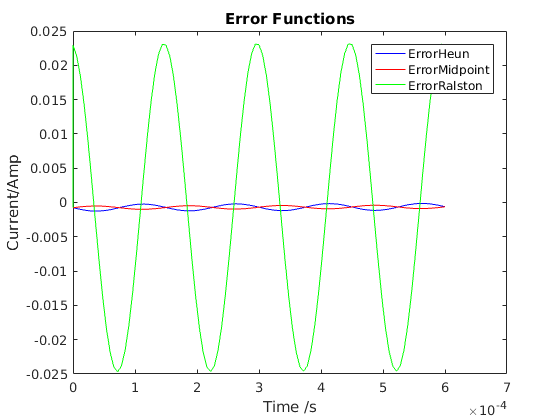
\includegraphics[width=\textwidth]{ex2/errorfunctions.png}
\caption{Error Functions}
\label{fig:ErrorFunctions}
\end{figure}

Looking at the plotted errors in Figure \ref{fig:ErrorFunctions} it is clear that the errors for all three numerical methods vary sinusoidally around the same amplitude just below $0$, with the Heun and Midpoint methods giving errors of the same magnitude in alternate phase and the Ralston method giving an error also varying sinusoidally but with a far greater magnitude.

\begin{figure}
\centering
      \begin{subfigure}{0.32\textwidth}
      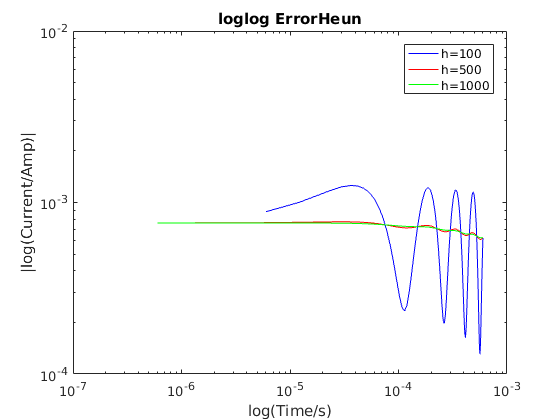
\includegraphics[width=\textwidth]{ex2/loglogerrorheun.png}
      \end{subfigure}
      \begin{subfigure}{0.32\textwidth}
      \includegraphics[width=\textwidth]{ex2/loglogerrormidpoint.png}
      \end{subfigure}
      \begin{subfigure}{0.32\textwidth}
      \includegraphics[width=\textwidth]{ex2/loglogerrorralston.png}
      \end{subfigure}
\caption{log-log plots}
\label{fig:llplots}
\end{figure}

As can be seen in Figure \ref{fig:llplots}, as the time step, $h$, is increased for the Midpoint and Heun methods the error remains varying around the same amplitude with the magnitude of the variance decreasing. Interestingly, as $h$ is increased for the Ralston method the variance of the error increases with the magnitude of the error itself decreasing. For all values of $h$, the error function has specific peaks and troughs at the same time values.

\subsubsection{error\_script.m}
\lstinputlisting[caption=error\_script.m]{ex2/error_script.m}



\newpage
\section{RLC Circuit}
Exercise 3 required the investigation of an RLC circuit and to try and simulate the system and produce plots of the output voltage of the system given a number of different input signals. These ranged from the Heaviside function to varying frequency Sine waves. The circuit investigated was as follows:

\begin{figure}[h]
\centering
\includegraphics[width=\textwidth]{ex3/RLCCircuit.png}
\caption{Given RLC Circuit}
\end{figure}

Given to us as well were the following equations for this particular circuit:

\begin{equation}\label{firstRLC}
v_{L}(t) + v_{R}(t) + v_{C}(t) = V_{in}(t)
\end{equation}

\begin{equation}\label{secondRLC}
L \frac{d}{dt}i_{L}(t) + Ri_{L}(t) + \frac{1}{C} \int_{0}^{t} i_{L}(t) = V_{in}(t)
\end{equation}

\begin{equation}\label{thirdRLC}
L \frac{d^2}{dt^2}qc(t) + R\frac{d}{dt}qc(t) + \frac{1}{C} qc(t) = V_{in}(t)
\end{equation}

Furthermore there were some initial conditions that would be used directly in the Matlab code such as the charge at $t_{0}$ and the values for the circuit components.

\subsection{Coupled Equations}\cite{coupledequations}

The first step required to implement the Runge-Kutta algorithm was to obtain the two coupled first order ODEs from the equations above. This could be done with some rearranging as follows:
\linebreak
\linebreak
If
\begin{equation}
y_{1} = qc(t)
\end{equation}
\begin{equation}
y_{2} = \frac{d}{dt}qc(t)
\end{equation}
\linebreak
Then $y_{1}$ prime must equal $y_{2}$, representing change in charge over time. The derivative of $y_{2}$ with respect to $t$ must then be $\frac{d^2}{dt^2}qc(t)$, representing change in current over time. Using all this the coupled equations become as follows:
\begin{equation}
y_{2}
\end{equation}
\begin{equation}
(V_{in}(t)-R\times y_{2}-\frac{y_{1}}{C})/L
\end{equation}
\linebreak
Equation 12 represents the change in charge over time and hence will be added to the initial charge value of 500nC. Equation 13 on the other hand shows the change in current over time and hence is added to the $y$ value representing initial current (initially a value of 0A at time $t_{0}$).
\linebreak
These can be seen in use regularly in the ``RLC Script" code.

\subsection{RLC\_Script}

\lstinputlisting[caption = RLC\_scipt.m]{ex3/RLC_script_small.m}


As can be seen in the code, for each new input signal, a new function is made to be passed by reference in the call to RK4second function. These new functions use the coupled equations outlined in the previous subsection. The values of the components of the circuit are initialised at the start of the file, along with the size of the arrays. Furthermore the arrays are 0 initialised.

There are for loops for each input signal that start from 2 (as the values of x and y at 1 are already given) and go to the calculated size of the array, given by the range over the step size. On each loop, a call to the RK4 second method is made and the parameters given are the previous x and y values, the initial time value for this loop, the two coupled equations and the step size. 

This function returns the next x and y values and when the for loop is done, we have a final value for $\frac{d}{dt}qc(t)$. All that is required to have a value for $V_{out}$ is to multiply by the resistance value.

Finally, a figure is produced for each input signal showing the input in red and the output voltage in black.
\newpage
\subsection{RK4second}

\lstinputlisting[caption = RK4second.m]{ex3/RK4second.m}

This function implements the Runge-Kutta 3/8 algorithm. The parameters taken in by this function were explained in the previous section. The first step is to assign the initial values to the final output values of $x$ and $y$ as they will be added to the values calculated in this function.

The main difference between this implementation and the classic 4th order Runge-Kutta is the weighting of the respective calculations at the end. For example, the classic implementation has a weighting of 1/6, 1/3, 1/3, 1/6. This adaptation has weightings of 1/8 for the two outer values and 3/8 for the inner ones, hence the name.\cite{rkequ}\cite{rkequ1}

Through some research, we found that due to the presence of two coupled equations, the implementation would be the same in terms of inside the brackets but the function/equation being called alternates.\cite{2equations} The value of the first coupled equation, y (current) is found first and then the result of the second equation is found ($\frac{d}{dt}i_{L}(t)/\frac{d^2}{dt^2}qc(t)$).

The results of the change in charge over time equation are added with the weightings taken into account to the initial $x$ value, representing charge at time $t_{0}$ with respect to that particular loop and the results of the second coupled equation, representing change in current over time, again with the weightings, are added to the initial current value. These values are returned.

\newpage
\subsection{Step Signal}

\begin{figure}[h]
\centering
\includegraphics[width=\textwidth]{ex3/Step_Signal.png}
\caption{Step Signal RLC}
\end{figure}

For the Heaviside function input, the voltage changes abruptly, from $0$ to $5V$ in this case, and so this change is not possible to be instantaneous across the capacitor, hence we get a transient response before we eventually settle down to the steady state response at around $0.02s$. The amplitude rises to a peak of about $2.3V$ at $0.002s$, but decreases in amplitude thereafter to its steady state of $0V$. The input signal can be seen moving from $0V$ to $5V$ at time $0s$.

\newpage
\subsection{Impulsive Signal with Decay}

\begin{figure}[h]
\centering
\includegraphics[width=\textwidth]{ex3/ImpulsiveSignal.png}
\caption{Impulsive Signal with Decay RLC}
\end{figure}

For an input of an impulsive signal with exponential decay, we have a similar shape to that seen for the step step signal, but the amplitudes are smaller, despite it seeming, from the plots, to reach its steady state at a very similar time of around $0.02s$. The peak amplitude here is $1.5V$ and it falls from there on with time. The gradient seems to have a relation with that of the input signal, with the drop in amplitude sharper at the start of the exponential decay as opposed to the end where the input signal has leveled off. The peak occurs between $0.001-0.002s$.

\newpage
\subsection{Square Waves}

Three separate square waves were examined in this section at three different frequencies: $5Hz$, $110Hz$ and $500Hz$.

\subsubsection{5Hz}

\begin{figure}[h]
\centering
\includegraphics[width=\textwidth]{ex3/Square_Wave_5_Hz.png}
\caption{Square Wave 5Hz RLC}
\label{fig:Square Wave 5Hz RLC}
\end{figure}


The first square wave investigated was one with a frequency of $5Hz$. The first thing to note is that the time axis extends a bit further than in previous plots. This is because a test was done at a $0.2s$ range and the outcome wasn't very clear showing only up to $0.2s$ and hence one cycle of the square wave, doubling the range gave the plot shown in Figure \ref{fig:Square Wave 5Hz RLC}. This plot really shows the effect of the transient as the input voltage changes abruptly from $+5V$ to $-5V$ and vice versa. A negative change brings about a largely negative transient amplitude as can be seen at $0.1s$ where the transient's amplitude falls to $-4.5V$. At $0.2s$, the opposite can be seen with a positive change in the input signal, a positive transient is seen with amplitude peaking at $+4.5V$. The transient effect seems to subside after $0.03s$ from the abrupt change and the steady state of $0V$ is reached. One other thing to note is that the amplitude reached by the transient is proportional to the change in the input signal. A good place to see this is at the start where the change is from $0V$ to $5V$ as opposed to the $10V$ swing seen later. This brings about a peak amplitude half the size of the others going up to only $2.2V$ as opposed to the usual $4.5V$.

\subsubsection{110Hz}

\begin{figure}[h]
\centering
\includegraphics[width=\textwidth]{ex3/Square_Wave_110_Hz.png}
\caption{Square Wave 110Hz RLC}
\end{figure}

At this higher frequency, the output is more resembling of a sine wave with the peaks at the centres of the squares in the square wave. The output polarity is correlated to that of the input with the negative half of the square wave cycle corresponding to a negative peak in the output. Apart from the first square wave cycle where the effects of the first abrupt change (a smaller jump than the later ones) leads to smaller peaks, the general trend of the peaks throughout is an amplitude $6.1V$ ($-6.1V$). This has a higher amplitude than the 5Hz square wave seen earlier. The reason the shape of this seems like a sine wave is perhaps that the while there is a transient effect, the change again is so quick that the current transient doesn't fade and reach its steady state before there is another abrupt change causing a new transient effect.

\newpage
\subsubsection{500Hz}

\begin{figure}[h]
\centering
\includegraphics[width=\textwidth]{ex3/Square_Wave_500_Hz.png}
\caption{Square Wave 500Hz RLC}
\end{figure}


The final square wave we looked at was one with a frequency of $500Hz$. The output voltage for this frequency had a number of features. Firstly it resembled a sawtooth wave, and the reason for this is probably similar to the reason for the $110Hz$ looking like a sine wave, the transient effect exists but it is short lived and cut off by a new abrupt change in the input voltage, and so it doesn't even get to the smooth curve at its peak seen at $5Hz$ or at $110Hz$. Hence the sharp change and the start of a new transient leads to the look of a sawtooth wave. The other key aspect is the amplitude, with a maximum (barring the start) of $1.2V-1.3V$. This is a lot lower than the amplitudes seen at $110Hz$.

\newpage
\subsection{Sine Waves}

Three separate square waves were examined in this section at three different frequencies: $5Hz$, $110Hz$ and $500Hz$.

\subsubsection{5Hz}

\begin{figure}[h]
\centering
\includegraphics[width=\textwidth]{ex3/Sine_Wave_5_Hz.png}
\caption{Sine Wave 5Hz RLC}
\end{figure}
 
Similar to the problem faced with the 5Hz square wave, the range needed to be slightly larger to see the full effects of this function as going up to about $0.2s$, the early transient and a not complete sine wave for the output signal meant that this was unclear, hence the extension to $0.4s$ (2 cycles). There is a transient as ever at the start due to the quick change in input voltage, but from then on, we seem to see a lower amplitude, phase shifted sine wave by about $90$ degrees (a cos wave essentially). A peak value of about $0.2V-0.3V$ means that the amplitude is a lot lower in comparison to the $5V$ of the original input signal. The transient causes an amplitude higher than that seen anywhere else but it reaches its steady state of a sine wave at about $0.03s-0.04s$.

\newpage
\subsubsection{110Hz}

\begin{figure}[h]
\centering
\includegraphics[width=\textwidth]{ex3/Sine_Wave_110_Hz.png}
\caption{Sine Wave 110Hz RLC}
\end{figure}

For the higher frequency of $110Hz$, we see that the output signal follows the input signal very closely beyond the first cycle of the sine wave with the amplitude almost exactly equal at $5V$, this is first fully exhibited at about $0.016s$, with previous peaks at $2.1V$($0.004s$), $-4.2V$($0.008s$) and $4.7V$($0.012s$). It is worth noting also that a wider range is not required here as a steady state output is seen very quickly as opposed to the earlier attempt at $5Hz$.

\subsubsection{500Hz}

\begin{figure}[ht]
\centering
\includegraphics[width=\textwidth]{ex3/Sine_Wave_500_Hz.png}
\caption{Sine Wave 500Hz RLC}
\end{figure}

For the last test of $500Hz$, we see that the output voltage is slightly out of phase with the input signal, more in line with what we saw at $5Hz$ rather than at $110Hz$. Furthermore, beyond the start at around $0.007s$ onwards, we see a steady peak amplitude of about $0.8V$, a lot less than what we saw at $110Hz$, and again more similar to the order of magnitude seen at 5Hz. Finally, again it takes less time still to see it reach a steady state with the range only needed to be $0.045s$ to see the effects fully as opposed to the larger ranges seen earlier, possibly a natural consequence of the higher frequency tested.

\subsection{Conclusion}

It is mentioned in the question given that these RLC circuits are usually used as band-pass filters, and if this is indeed the case the results may back this point. Looking at the amplitudes for both the square wave tests and the sine wave tests, it is clear that at $110Hz$, the amplitude is a lot larger in comparison to $5Hz$ and $500Hz$ in both types of signal. This may imply that if this is indeed a band pass filter, $110Hz$ is almost certainly within the band of frequencies allowed to pass through by this filter, with $5Hz$ and $500Hz$ both falling within the ranges outside and hence attenuated, hence the lower amplitudes seen.


\newpage
\section{Finite Differences for PDE}

\subsection{Solving heat equations}
The 1-D heat equation: 
\[\frac{\partial y}{\partial t} = \frac{\partial^2 y}{\partial x^2}, \qquad 0<x<1, \quad t>0\]
with boundary conditions $y(0,t) = y(1,t) = 0$, and initial condition $y(x,0) = y_0(x)$ describes the temperature distribution in a thin metal rod of length 1, with insulated sides and both ends kept at temperature zero. At time $t = 0$, the distribution is $y_0(x)$ and the solution of the PDE describes the evolution in time. The PDE can also be used to describe other diffusive processes, for example, pollutant gas in a pipe, or a random walk.\cite{mathlecturenotes}

This can be solved numerically using finite difference method.

For spatial derivative, central difference method is used:
\[
      \frac{\partial^2 y(x,t)}{\partial x^2} \approx \frac{y(x+h,t)-2y(x,t)+y(x-h,t)}{h^2}      
\]
where only $x$ varies by $h$ in both directions, and $t$ stays constant. So when $x=x_j$ and $t=t_m$, we have $x \pm h = x_{j \pm 1}$:
\begin{align*}
      \frac{\partial^2 y(x_j,t_m)}{\partial x^2} &\approx \frac{y(x_{j+1},t_m)-2y(x_j,t_m)+y(x_{j-1},t_m)}{h^2}\\
      &= \frac{U_{j+1}^{m}-2U_{j}^{m}+U^m_{j-1}}{h^2}, \qquad j=1,2,...N-1
\end{align*}
For the time derivative, ``forward difference" is used since negative time is not allowed.
\begin{align*}
      \frac{\partial y(x_j,t_m)}{\partial t} &\approx \frac{y(x_j,t_{m+1})-y(x_j,t_m)}{k}\\
      &= \frac{U^{m+1}_j-U^m_j}{k}, \qquad m=0,1,2,3...
\end{align*}
Set the two derivatives equal:
\[
      \frac{U^m_{j+1}-2U^m_j+U^m_{j-1}}{h^2}=\frac{U^{m+1}_j - U^m_j}{k}
\]
Let $\frac{k}{h^2}=v$ and rearrange to:
\[
      v(U^m_{j+1}-2U^m_j+U^m_{j-1})=U^{m+1}_j - U^m_j
\]
There is only one term at time $t_{m+1}$. Knowing $U^0_j$, from the initial condition, $U^1_j$ can be found from the last equation rearranged as:
\[
      U^{m+1}_j=vU^m_{j-1}+(1-2v)U^m_j+vU^m_{j+1}
\]
\subsubsection{finite\_script.m}
\textbf{finite\_script.m} is written to implement the finite difference method.

It iterates through time intervals. During each iteration, the state(temperature, in this case) of each spatial interval is calculated. The iteration stops when the end condition is met, that is number of iterations in total. The time it takes to develop to a specific heat state can be expressed as: $k\times iterations$, see below for definitions.

The script can take boundary conditions that vary with time. The function takes the following arguments:\\
\indent \indent $k$: the time interval\\
\indent \indent $iterations$: iterations in time\\
\indent \indent $h$: spatial interval\\
\indent \indent $x0, xf$: spatial range\\
\indent \indent $init$: function handle to initial condition\\
\indent \indent $bcl$: function handle to left boundary condition\\
\indent \indent $bcr$: function handle to right boundary condition

\lstinputlisting[caption = finite\_scipt.m]{ex4/finite_script.m}

\newpage
\subsubsection{$Tent$ Function as the initial condition}
The initial condition is:
\[ y_0(x)=
	\begin{cases} 
      2x & 0\leq x < 0.5 \\
      2-2x & 0.5\leq x\leq 1 \\
   \end{cases}
\]
The rod has the highest temperature at the center, and the sides are kept at zero.

As time evolves, the whole rod cools down. Higher temperature has higher decrease rate.

\begin{figure}[h]
\centering
\includegraphics[width=\textwidth]{ex4/plots/tent.png}
\caption{A rod with tent initial condition, as shown in blue trace}
\end{figure}

\lstinputlisting[caption = solve heat equation for tent]{ex4/driver_tent.m}

\newpage
\subsubsection{$Sine$ Function as the initial condition}
The initial condition is:
\[ y_0(x)= sin(2\pi x) \]
The rod has three points at zero temperature. Since the left and right part of the rod has temperature equal in amplitude, but opposite in sign, the heat transfer from left and to right cancel each other. So no temperature change occurs at the mid point.

\begin{figure}[h]
\centering
\includegraphics[width=\textwidth]{ex4/plots/sine.png}
\caption{A rod with sine initial condition, as shown in blue trace}
\end{figure}
\lstinputlisting[caption = solve heat equation for sine]{ex4/driver_sin.m}

\newpage
\subsubsection{$y=(x-0.5)^2$ as the initial condition}
Temperature in the middle is lower than the sides. Heat diffuses to the middle so that the temperature rises, but it never exceeds the sides.

\begin{figure}[h]
\centering
\includegraphics[width=\textwidth]{ex4/plots/custom_cup.png}
\caption{A rod with cold middle and hot sides initial condition, as shown in blue trace}
\end{figure}
\lstinputlisting[caption = solve heat equation for cup shape]{ex4/driver_custom_cup.m}

\newpage
\subsubsection{$y=-(x^2)+1$ as the initial condition}
The whole rod cools down as expected. One thing to notice is that the left side has much higher temperature at the beginning, so its temperature drop is much faster. But the two sides tend to the same temperature after a while.

\begin{figure}[h]
\centering
\includegraphics[width=\textwidth]{ex4/plots/custom_mountain.png}
\caption{A rod with hot left side and cold right side initial condition, as shown in blue trace}
\end{figure}
\lstinputlisting[caption = solve heat equation for mountain shape]{ex4/driver_custom_mountain.m}

\newpage
\subsection{Bonus Exercise}
This section builds upon the PDE Solution
\subsubsection{Initial condition that does not match boundary
conditions}
The initial conditions being used are:

\[ y_0(\textit{x})=
	\begin{cases} 
      2x & 0\leq x < 0.5 \\
      2-x & 0.5\leq x\leq 1 \\
   \end{cases}\]
\newline

This does not match the right boundary condition, and results in the following plot:

\begin{figure}[h]
\centering
\includegraphics[width=\textwidth]{exbonus/tent1.png}
\caption{A rod with initial conditions not matching boundary conditions, as shown in blue trace}
\end{figure}
\newpage
\lstinputlisting[caption = solve heat equation for initial conditions not matching boundary conditions]{exbonus/driver_bonus1.m}


\newpage
\subsubsection{Constant, non-zero boundary conditions}
The initial conditions being used are:

\[ y_0(\textit{x})=
	\begin{cases} 
      2x & 0\leq x\leq 0.5 \\
      2-2x & 0.5\leq x\leq 1 \\
   \end{cases}\]


\begin{figure}[h]
\centering
\includegraphics[width=\textwidth]{exbonus/constbound.png}
\caption{A rod with tent initial conditions, as shown in blue trace. The boundary conditions are y=1 for both ends}
\end{figure}
\lstinputlisting[caption = solve heat equation for constant boundary conditions]{exbonus/driver_bonus2.m}

\newpage
\subsubsection{Time-varying boundary conditions}
The initial conditions being used are:

\[ y_0(\textit{x})=
	\begin{cases} 
      2x & 0\leq x\leq 0.5 \\
      2-2x & 0.5\leq x\leq 1 \\
   \end{cases}\]


The left and right boundary conditions are \(y=10x\)

\begin{figure}[h]
\centering
\includegraphics[width=\textwidth]{exbonus/timebound.png}
\caption{A rod with tent initial conditions, as shown in blue trace. The boundary conditions are y=10x for both ends}
\end{figure}
\lstinputlisting[caption = solve heat equation for time-varying boundary conditions]{exbonus/driver_bonus3.m}



\newpage


\begin{thebibliography}{9}

\bibitem{mathlecturenotes}
Daniel Nucinkis (2016/17)
\textit{EE2-8C Mathematics Numerical Analysis of Differential Equations}
Available from: \texttt{https://bb.imperial.ac.uk}[Accessed \printdate{2017-03-01}]

\bibitem{rlcircuitprove}
Electrical4u
\textit{RL Series Circuit}
Available from: \texttt{https://www.electrical4u.com/rl-series-circuit}[Accessed \printdate{2017-03-12}]

\bibitem{lrtransient} 
AspenCore, Inc
\textit{RL circuit transient}
Available from: \texttt{http://www.electronics-tutorials.ws/inductor/lr-circuits.html}[Accessed \printdate{2017-03-11}]

\bibitem{waveformoutput} 
Integrated Publishing, Inc.
\textit{RL circuit}
Available from: \texttt{http://www.tpub.com/neets/book9/36j.htm}[Accessed \printdate{2017-03-12}]

\bibitem{coupledequations} NC State University. (n.d.). Lesson 12: LRC Circuit, Tuning and ode45. Available from: http://www4.ncsu.edu/eos/users/w/white/www/white/ma302/less1208.pdf. Accessed 13th March 2017. 
Used to find coupled equations and understand what they represent.
\bibitem{2equations} Calvin College. (n.d.). MATH 231A Runge-Kutta Notes: for a 2-equation, 1st-order system. Available from: https://www.calvin.edu/~scofield/courses/m231/materials/rungeKuttaFormulas.pdf. Accessed 13th March 2017.

Used to look at how to extend the Runge-Kutta algorithm using two coupled equations rather than one.
\bibitem{rkequ} RLH. (n.d.). Runge-Kutta 3/8 Method. Available from: http://www.mymathlib.com/diffeq/runge-kutta/runge\_kutta\_3\_8.html. Accessed 13th March 2017. 

Used to find the Runge-Kutta 3/8 Algorithm.
\bibitem{rkequ1} The MathWorks, Inc. (2015). Solving ODEs in MATLAB, 3: Classical Runge-Kutta, ODE4. Available from: https://uk.mathworks.com/videos/solving-odes-in-matlab-3-classical-runge-kutta-ode4-117528.html. Accessed 13th March 2017.

Used to see an example of how to implement the Classic Runge-Kutta in Matlab. The Mathworks website was generally used extensively to check the syntax for Matlab coding.

\end{thebibliography}

\end{document}
